%%%%%%%%%%%%%%%%%%%%%%%%%%%%%%%%%%%%%%%%%
% Masters/Doctoral Thesis 
% LaTeX Template
% Version 2.5 (27/8/17)
%
% This template was downloaded from:
% http://www.LaTeXTemplates.com
%
% Version 2.x major modifications by:
% Vel (vel@latextemplates.com)
%
% This template is based on a template by:
% Steve Gunn (http://users.ecs.soton.ac.uk/srg/softwaretools/document/templates/)
% Sunil Patel (http://www.sunilpatel.co.uk/thesis-template/)
%
% Template license:
% CC BY-NC-SA 3.0 (http://creativecommons.org/licenses/by-nc-sa/3.0/)
%
%%%%%%%%%%%%%%%%%%%%%%%%%%%%%%%%%%%%%%%%%

%----------------------------------------------------------------------------------------
%	PACKAGES AND OTHER DOCUMENT CONFIGURATIONS
%----------------------------------------------------------------------------------------

\documentclass[
11pt, % The default document font size, options: 10pt, 11pt, 12pt
%oneside, % Two side (alternating margins) for binding by default, uncomment to switch to one side
english, % ngerman for German
onehalfspacing, % alternatives: singlespacing, onehalfspacing or doublespacing
%draft, % Uncomment to enable draft mode (no pictures, no links, overfull hboxes indicated)
%nolistspacing, % If the document is onehalfspacing or doublespacing, uncomment this to set spacing in lists to single
%liststotoc, % Uncomment to add the list of figures/tables/etc to the table of contents
%toctotoc, % Uncomment to add the main table of contents to the table of contents
%parskip, % Uncomment to add space between paragraphs
%nohyperref, % Uncomment to not load the hyperref package
headsepline, % Uncomment to get a line under the header
%chapterinoneline, % Uncomment to place the chapter title next to the number on one line
% consistentlayout, % Uncomment to change the layout of the declaration, abstract and acknowledgements pages to match the default layout
]{MastersDoctoralThesis} % The class file specifying the document structure

\usepackage[utf8]{inputenc} % Required for inputting international characters
\usepackage[T1]{fontenc} % Output font encoding for international characters


\usepackage{nicematrix}
\usepackage[demo]{rotating}

\usepackage{mathpazo} % Use the Palatino font by default

\usepackage[backend=bibtex,style=authoryear,natbib=true]{biblatex} % Use the bibtex backend with the authoryear citation style (which resembles APA)

\addbibresource{report.bib} % The filename of the bibliography

\usepackage[autostyle=true]{csquotes} % Required to generate language-dependent quotes in the bibliography

\newcommand{\keyword}[1]{\textbf{#1}}
\newcommand{\tabhead}[1]{\textbf{#1}}
\newcommand{\code}[1]{\texttt{#1}}
\newcommand{\file}[1]{\texttt{\bfseries#1}}
\newcommand{\option}[1]{\texttt{\itshape#1}}

%----------------------------------------------------------------------------------------
%	MARGIN SETTINGS
%----------------------------------------------------------------------------------------

\geometry{
	paper=a4paper, % Change to letterpaper for US letter
	inner=2.5cm, % Inner margin
	outer=3.8cm, % Outer margin
	bindingoffset=.5cm, % Binding offset
	top=1.5cm, % Top margin
	bottom=1.5cm, % Bottom margin
	%showframe, % Uncomment to show how the type block is set on the page
}

%----------------------------------------------------------------------------------------
%	THESIS INFORMATION
%----------------------------------------------------------------------------------------

\thesistitle{Bespoke Customer Relationship Management and Point of Sale System} % Your thesis title, this is used in the title and abstract, print it elsewhere with \ttitle
\supervisor{Dr. Khuong An \textsc{Nguyen}} % Your supervisor's name, this is used in the title page, print it elsewhere with \supname
\examiner{} % Your examiner's name, this is not currently used anywhere in the template, print it elsewhere with \examname
\degree{Computer Science BSc} % Your degree name, this is used in the title page and abstract, print it elsewhere with \degreename
\author{Jazer \textsc{Barclay}} % Your name, this is used in the title page and abstract, print it elsewhere with \authorname
\addresses{} % Your address, this is not currently used anywhere in the template, print it elsewhere with \addressname

\subject{Computer Science} % Your subject area, this is not currently used anywhere in the template, print it elsewhere with \subjectname
\keywords{} % Keywords for your thesis, this is not currently used anywhere in the template, print it elsewhere with \keywordnames
\university{\href{https://www.brighton.ac.uk/}{University of Brighton}} % Your university's name and URL, this is used in the title page and abstract, print it elsewhere with \univname
\department{\href{https://www.brighton.ac.uk/}{School of Architecture, Technology and Engineering}} % Your department's name and URL, this is used in the title page and abstract, print it elsewhere with \deptname
\faculty{\href{http://faculty.university.com}{Faculty Name}} % Your faculty's name and URL, this is used in the title page and abstract, print it elsewhere with \facname

\AtBeginDocument{
\hypersetup{pdftitle=\ttitle} % Set the PDF's title to your title
\hypersetup{pdfauthor=\authorname} % Set the PDF's author to your name
% \hypersetup{pdfkeywords=\keywordnames} % Set the PDF's keywords to your keywords
}

\begin{document}

\frontmatter % Use roman page numbering style (i, ii, iii, iv...) for the pre-content pages

\pagestyle{plain} % Default to the plain heading style until the thesis style is called for the body content

%----------------------------------------------------------------------------------------
%	TITLE PAGE
%----------------------------------------------------------------------------------------

\begin{titlepage}
\begin{center}

\vspace*{.04\textheight}
{\includegraphics[
	width=14cm,
	height=6cm,
	keepaspectratio,
	]{Logo}\par}\vspace{.8cm} % University/department logo - uncomment to place it
%{\scshape\LARGE \univname\par}\vspace{1.5cm} % University name
\textsc{\Large Final Year Project\\[.2cm]Dissertation Report}\\[.8cm] % Thesis type

\HRule \\[0.4cm] % Horizontal line
{\huge \bfseries \ttitle\par}\vspace{0.4cm} % Thesis title
\HRule \\[1.5cm] % Horizontal line

\begin{minipage}[t]{0.4\textwidth}
	\begin{flushleft} \large
		\emph{Author:}\\
		\href{https://www.jazer.dev/}{\authorname}\\ % Author name - remove the \href bracket to remove the link
	\end{flushleft}
\end{minipage}
\begin{minipage}[t]{0.4\textwidth}
	\begin{flushright} \large
		\emph{Supervisor:} \\
		\href{https://research.brighton.ac.uk/en/persons/khuong-nguyen}{\supname}
	\end{flushright}
\end{minipage}\\[.7cm]



\begin{minipage}[t]{0.4\textwidth}
	\begin{flushleft} \large
		\emph{Student ID:}\\
		\href{mailto:j.barclay3@uni.brighton.ac.uk}{20837308}\\
	\end{flushleft}
\end{minipage}
\begin{minipage}[t]{0.4\textwidth}
	\begin{flushright} \large
		\emph{Second Reader:} \\
		\href{https://www.researchgate.net/profile/Saeed-Malekshahi-Gheytassi}{Dr. Saeed Malekshahi \textsc{Gheytassi}}
	\end{flushright}
\end{minipage}\\[1.5cm]


\large \textit{A dissertation submitted in fulfilment of the requirements\\ for the degree of \degreename}\\[0.3cm] % University requirement text
\textit{at the}\\[0.4cm]
\univname\\\deptname\\[1cm] % Research group name and department name

{\large \today}\\[1cm] % Date

\end{center}
\end{titlepage}

%----------------------------------------------------------------------------------------
%	DECLARATION PAGE
%----------------------------------------------------------------------------------------

\begin{declaration}
\addchaptertocentry{\authorshipname} % Add the declaration to the table of contents
\noindent I hereby declare that this thesis titled, \enquote{\ttitle} and the work presented in it are my own. I confirm that:

\begin{itemize} 
\item This work was done wholly or mainly while in candidature for a research degree at this University.
\item Where any part of this thesis has previously been submitted for a degree or any other qualification at this University or any other institution, this has been clearly stated.
\item Where I have consulted the published work of others, this is always clearly attributed.
\item Where I have quoted from the work of others, the source is always given. With the exception of such quotations, this thesis is entirely my own work.
\item I have acknowledged all main sources of help.
\item Where the thesis is based on work done by myself jointly with others, I have made clear exactly what was done by others and what I have contributed myself.
\end{itemize}

\hspace{-1cm}

% \begin{minipage}[t]{0.95\textwidth}
% 	\begin{flushright} \large
% 		\emph{\authorname} \\
% 		\emph{\today} \\
% 	\end{flushright}
% \end{minipage}\\[1.5cm]

% \begin{minipage}[t]{0.95\textwidth}
% 	\begin{flushleft} \large
% 		\emph{Name:} \\
% 		\emph{Date:} \\
% 	\end{flushleft}
% \end{minipage}\\[1.5cm]

\noindent \begin{minipage}[t]{0.5\textwidth}
	\begin{flushleft} \large
		\emph{Student Name:}\\[.4em]
		\authorname\\
		\rule[0.5em]{10em}{0.5pt}
	\end{flushleft}
\end{minipage}
\noindent \begin{minipage}[t]{0.5\textwidth}
	\begin{flushright} \large
		\emph{Date:} \\[.4em]
		\today\\
		\rule[0.5em]{10em}{0.5pt}
	\end{flushright}
\end{minipage}\\[.2em]




% \noindent \authorname \\
% \rule[0.5em]{25em}{0.5pt} % This prints a line for the signature
 
% \noindent Date: \today \\
% \rule[0.5em]{25em}{0.5pt} % This prints a line to write the date

\end{declaration}

\cleardoublepage

%----------------------------------------------------------------------------------------
%	ACKNOWLEDGEMENTS
%----------------------------------------------------------------------------------------

\begin{acknowledgements}
\addchaptertocentry{\acknowledgementname} % Add the acknowledgements to the table of contents

\vspace*{.03\textheight}

\hspace{\parindent} To my supervisor, \supname, for his guidance through university while on my learning journey. He has inspired curiosity through showmanship, sparked a dedication to excellence to achieve my scholarship and to conduct myself professionally in my project.\\

To my scholarship mentor, Sam Innes, for showing how far I can push myself and giving me a vision of my future potential career.\\

To all of my friends for keeping me on track with my work and giving me the opportunity to teach while learning.\\

To my girlfriend, Sophie Leanne Ryan, for her emotional support and charity of time.\\

To my parents for their love and support through my life, teaching me hard lessons early and being there to catching me when I fall.

\end{acknowledgements}

%----------------------------------------------------------------------------------------
%	ABSTRACT PAGE
%----------------------------------------------------------------------------------------

\begin{abstract}
\addchaptertocentry{\abstractname} % Add the abstract to the table of contents
\hspace{\parindent} A small, local kickboxing company is experiencing explosive growth; however, they are losing money due to inefficient tracking of customers, attendance and purchases.\\

The business requires a customer relationship management system to resolve these issues by accurately maintaining customer records, lesson purchases and attendance data. It must also meet the business' complex pricing requirements to hold precise purchase records.\\

Development and implementation of this bespoke software artefact has increased profits by over 200\%, efficiency in receptionist work increased by 400\%, and tax return calculation time decreased from 2-3 days to 4 hours.
\end{abstract}

%----------------------------------------------------------------------------------------
%	LIST OF CONTENTS/FIGURES/TABLES PAGES
%----------------------------------------------------------------------------------------

\tableofcontents % Prints the main table of contents

\listoffigures % Prints the list of figures

\listoftables % Prints the list of tables

%----------------------------------------------------------------------------------------
%	THESIS CONTENT - CHAPTERS
%----------------------------------------------------------------------------------------

\mainmatter % Begin numeric (1,2,3...) page numbering

\pagestyle{thesis} % Return the page headers back to the "thesis" style

% Include the chapters of the thesis as separate files from the Chapters folder
% Uncomment the lines as you write the chapters

%----------------------------------------------------------------------------------------
%	Introduction
%----------------------------------------------------------------------------------------
\chapter{Introduction} % Main chapter title
\label{Chapter1} % For referencing the chapter elsewhere, use \ref{Chapter1} 

In this chapter, we introduce the business and the problems they face. Next, we cover the project motivations for solving these issues and the resulting objectives. We then go over what lies outside this project's scope, and finally, we will summarise this document's overall structure covering each chapter in detail.

%----------------------------------------------------------------------------------------
%	1. Project motivation
%----------------------------------------------------------------------------------------
\section{Project motivation}
Up-grade Martial Arts (UMA) is a small, local gym offering boxing, kickboxing and yoga services. On top of this, they provide space for coaches to train members in one-to-one lessons. In addition to regular customers, they support adults and juniors with physical or learning disabilities to help improve their hand-eye and mental coordination through regular training and practice.\\

\begin{figure}[h!]
    \centerline{
\includegraphics[width=0.45\linewidth]{uma-logo.png}}
    \caption{Up-grade Martial Arts Logo}
    \label{fig:umalogo}
\end{figure}

The business is growing fast with an influx of new members signing up for the gym, and they have observed double the average number of attendees for lessons. This growth has had a knock-on effect on the business and interaction with its existing system.

\textbf{Lesson sizes were getting too big for the gym space}. The growth in members attending has resulted in larger lesson sizes which are unmanageable in a small location. The business responded by increasing the number of lessons available during the day, which has led to more problems.

\textbf{Net income has not increased at the same rate as membership growth}. Although more members are attending, net income and profit have not seen the same increase. When cross-referenced with payments, an analysis of the attendance records shows that members attend lessons without paying. After further examination, receptionists expressed confusion about what members had paid for monthly bulk purchases and when they expired.

\textbf{Receptionist remains part-time due to low increase in revenue}. With the increased working hours and the limited increase in revenue, the receptionist can only be employed part-time. As a result, other staff members are administering the currently improvised system.

\textbf{Inconsistencies and errors in data input}. Due to more staff being involved in using the existing system, it has broken down with data input becoming inconsistent, longer member information lookup times and, in extreme cases, data loss due to misplaced forms or unsaved changes in spreadsheets.

\textbf{With larger and numerous lessons also comes the issue of health and safety}. With more members attending lessons, especially members with learning disabilities and juniors, maintaining accurate records of members and what lessons they attend is vital in an emergency such as an injury or fire. Due to the manual searching of unorganised paper records, the current speed for member information lookup can range anywhere from 30 seconds to 3 minutes.

\textbf{Ultimately, the current system is unsustainable with growth}. This system consisting of pen-and-paper member records in combination with attendance spreadsheets and printout price lists has become the crux of all these issues. The system cannot scale with the business needs and has cost them a considerable financial amount. For these reasons, a new system has been implemented to solve these issues and assist the business in its growth. 


%----------------------------------------------------------------------------------------
%	2. Project objectives
%----------------------------------------------------------------------------------------
\section{Project objectives}
The primary objectives of this project have been to build a bespoke system that tracks and accurately stores business-critical data, meets the business' complex pricing requirements and provides valuable analytical data for making informed business decisions. In addition, this new system must unify the data entry method and provide insightful analytic data using the stored data.

Considerations for accessibility, ease of use and searchability are vital to a system working with vast amounts of data. In addition, care must be taken to prevent erroneous data entry, error states and problems associated with multi-user access.

The primary objectives of this project included the following:
\begin{itemize}
    \item \textbf{Ease of use and searchability} - receptionists must be able to find member information within 5 seconds and attendance for a lesson within 10 seconds. The current system takes over a minute to find, which is unacceptable in an emergency.
    \item \textbf{Track members, their purchases and lesson attendance} - managers and receptionists need suitable storage of this information to ensure members have paid for the lessons they attend.
    \item \textbf{Allow accessibility across multiple and different devices} - receptionists will use this system on-premises; however, managers will need access to statistics from any location at any time.
    \item \textbf{Provide valuable and insightful analytics} - managers must complete tax returns involving total income for a given period and make informed business decisions based on member signup and attendance data.
\end{itemize}



%----------------------------------------------------------------------------------------
%	3. Limitations of scope
%----------------------------------------------------------------------------------------
\section{Limitations of scope}

Due to the extensive scope of this project, non-critical components and future considerations were omitted. However, these can be explored as additional features after the project's completion. The limitations include the following:
\begin{itemize}
    \item \textbf{Expense tracking} - The business has many outgoing payments, which vary in amount, service, method and many more. It would significantly increase the functional requirements to include this functionality and does not relate to customer relationship management.
    \item \textbf{Member login access to the system} - Different access levels would complicate the system, increasing the signup function's complexity. The added surface area for an attack would also negatively impact the system, especially for a short development project.
    \item \textbf{Considerations for multi-site} - With plans to expand once income increases, the system may need to support multiple sites. Although the system is online, specific handling of sites and spaces is an optional feature that can be considered in the future.
    \item \textbf{Interaction with the cash draw and printer} - Access to physical devices would require accompanying software to connect and provide control. This functionality would result in two separate pieces of software. 
    \item \textbf{Interaction with online card payment systems} - A card payment system is already in operation, though it does not support API interaction to integrate.
\end{itemize}



%----------------------------------------------------------------------------------------
%	4. Dissertation outline
%----------------------------------------------------------------------------------------
\section{Dissertation outline}

In this chapter, \textbf{Chapter 1}, we have introduced the business and its problems, the objectives which the software artefact must cover and what lies out of scope in this work. In the next chapter, \textbf{Chapter 2}, we will cover the research conducted into the operations and ethos of Up-grade Martial Arts and competitor analysis of existing software completed during the planning stages. \textbf{Chapter 3} discusses the development methodology utilised and tools employed during development. \textbf{Chapter 4} covers the complete architecture of the system, starting with a top-down view and then moving into each component's design and implementation. \textbf{Chapter 5} details the project's management throughout its lifecycle and the testing conducted to ensure correct operation. \textbf{Chapter 6} discusses considerations for the software's legal, social and ethical impact. Finally, we conclude with \textbf{Chapter 7}, a reflection on the process, the final software product and future considerations should this project be continued post-graduation. % Introduction
%----------------------------------------------------------------------------------------
%	Literature research
%----------------------------------------------------------------------------------------
\chapter{Literature research} % Main chapter title
\label{Chapter2} % For referencing the chapter elsewhere, use \ref{Chapter2}

This chapter covers the in-depth research conducted on up-grade martial arts and examines the suitability of off-the-shelf software solutions for customer relationship management for the business.

%----------------------------------------------------------------------------------------
%	1. Company research
%----------------------------------------------------------------------------------------

\section{Company research}
Building a bespoke system requires tailoring to the business and its operations. Therefore, information gathering was essential to ensure the new software fits within their ecosystem. 

\subsection{Meetings}

Research began through an initial meeting with the business owners. In this session, we discussed their problem and potential solutions. The final solution was to develop a single system accessible from any location that unifies the data storage and searching of business-critical data.


\begin{table}[ht!]
    \renewcommand{\arraystretch}{1.5}
    \label{fig:meetingtable}
    \caption{Problems the business faces and the proposed solutions}
    \centerline{
        \begin{NiceTabular}{ m{4.5cm} m{3.6cm} m{4.5cm}  }
            \hline
            \textbf{Problem} & \textbf{Domain} & \textbf{Solution}\\
            \hline \hline
            Fragmented system & Operational & Condense all processes into a single system \\
            \hline
            Slow member signup & Functional & Create digital signup \\
            \hline
            Inconsistent input & Data & Standardised input display and method \\
            \hline
            Slow member search & Health and Safety & Create easy lookup through table \\
            \hline
            Statistics takes too long to calculate & Business & Have stats calculated on-the-fly clearly visible \\
            \hline
            No method of cross-referencing member attendance with payments & Financial & Use a token system which are valid for single use across a time range \\
            \hline
           \end{NiceTabular}
    }
\end{table}


\subsection{User stories}
In subsequent discovery sessions, requirements, user stories and wireframes were created to consolidate the system's operations and boundaries, preventing feature creep.

\begin{table}[ht!]
    \renewcommand{\arraystretch}{1.2}
    \label{fig:userstories}
    \caption{User stories}
    \centerline{
        \begin{NiceTabular}{ m{3.3cm} m{4.6cm} m{5cm}  }
            \hline
            \textbf{Action} & \textbf{Process} & \textbf{Result}\\
            \hline \hline
            Login & Validate and verify details & Provide or deny access to the system \\
            \hline
            View members & Go to members page & Table showing all members. Click reveals all detials \\
            \hline
            Add members & Go to members page, fill in form, submit & New member shows in table \\
            \hline
            Edit members & Go to members page, click member to edit, update and submit & Member details update in table \\
            \hline
            View Lessons & Go to lessons page & Table showing all lessons. Click reveals all detials \\
            \hline
            Add Lessons & Go to lessons page, fill in form, submit & New lesson shows in table \\
            \hline
            Edit Lessons & Go to lessons page, click member to edit, update and submit & Lesson details update in table \\
            \hline
            View Attendance & Go to attendance page, select lessons & Table showing all attendances for selected lesson \\
            \hline
            Add Attendance Free & Go to attendance page, select lesson, select member, click add & Attendance added \\
            \hline
            Add Attendance Pay Now & Go to attendance page, select lesson, select member, click add & Payment prompted, pay now selected \\
            \hline
            Add Attendance Pay Later & Go to attendance page, select lesson, select member, click add & Payment promoted, pay later selected \\
            \hline
            View bulk purchase & Go to purchase page & Table showing all prices for lessons \\
            \hline
            Add bulk purchases & Go to purchase page, select member, select purchase plan & confirm payment, log transaction \\
            \hline
            View Payments & Go to payments page & Table showing all payments for all lessons \\
            \hline
            View statistics & Go to dashboard page & All statistics viewable in single page \\
            \hline
           \end{NiceTabular}
    }
\end{table}


\subsection{Document acquisition}
Document acquisition was also a crucial part of the research. Publicly available resources were collected alongside internal material. Documents included price lists (Appendix \ref{AppendixC:PriceList}), member signup form (Appendix \ref{AppendixC:SignupForm}) and attendance spreadsheets (Appendix \ref{AppendixC:AttendanceSpreadsheet}). The personally identifiable information was redacted, so only the structures remained.

Copyrighted content, such as logos and colour schemes from their website, would heavily influence the design. Consequently, written permission was requested from all business owners and was confirmed at the beginning of development (Figure~\ref{fig:consent}).

\begin{figure}[ht!]
    \centerline{\fbox{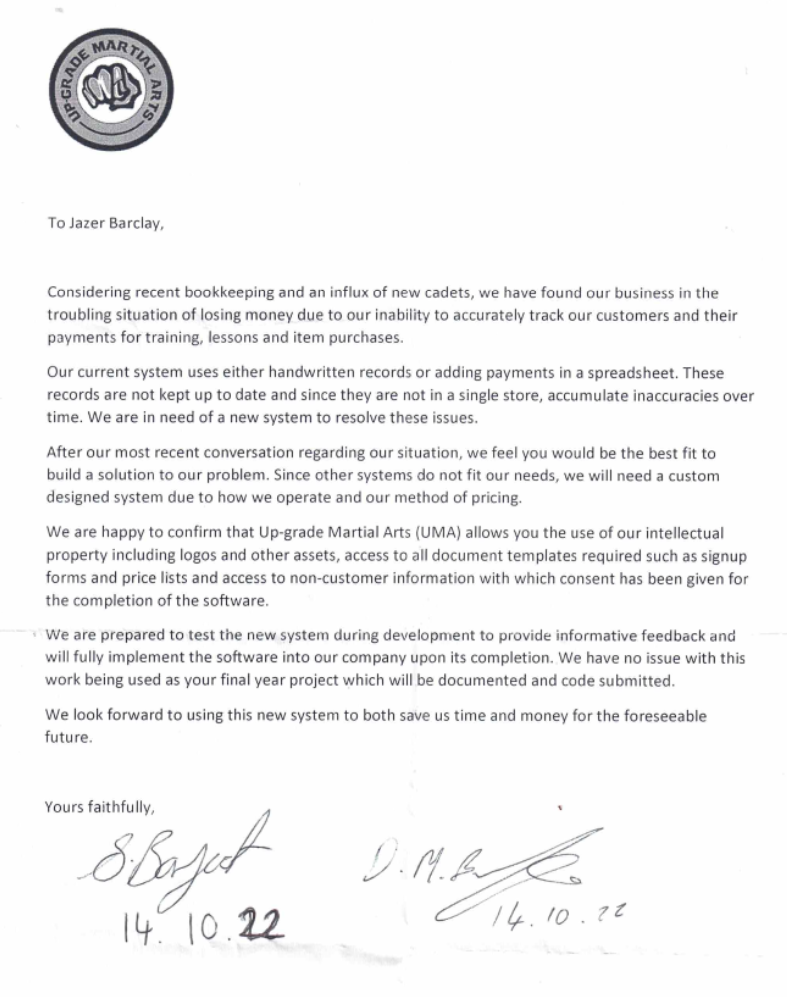
\includegraphics[width=.75\linewidth]{consent.png}}}
    \caption{Consent to create the application and use business copyrighted assets during development}
    \label{fig:consent}
\end{figure}


\subsection{Results of research}
The in-depth research into the business reveals a system that started small with new elements and features added without considering expansion over time. The fragmented nature creates friction between the end user and the data.

%----------------------------------------------------------------------------------------
%	2. Competitor analysis
%----------------------------------------------------------------------------------------

\section{Competitor analysis}
Off-the-shelf customer relationship management software exists for general-purpose use. These are designed for small to medium-sized businesses with a more generic approach to business operations.

The leading software in the space are InvoiceNinja \parencite{noauthor_invoice_nodate} and HubSpot \parencite{noauthor_hubspot_2022}. Both boast being free with premium pricing plans for access to more advanced and comprehensive tools, many of which the business requires.

UMA has tested many CRM and Point-of-Sale (PoS) systems in the past; however, due to their complex pricing and lesson structure, many fall short of their extensive requirements or require two separate systems to operate.

Attempts to use this software have resulted in even greater confusion, and business data has become fragmented across all systems.

A more critical study compared and contrasted the leading software currently on the market to further the research into existing software found in Table~\ref{fig:soft-comp}.

\begin{table}[ht!]
    \caption{Off-the-shelf software comparison based on features}
    \renewcommand{\arraystretch}{2}
    \centerline{
        \begin{NiceTabular}{ m{2.2cm} m{4cm} m{4cm} m{2cm}  }
            \hline
            \textbf{Feature} & \textbf{HubSpot} & \textbf{Invoice Ninja} & \textbf{Best Fit}\\
            \hline \hline
            Customer input & Complex to setup however supports the required field very well & Easy to input however limited on fields available & Both\\
            \hline
            Customer search & Advanced search tools available but requires setup & Simple search based on fixed fileds & HubSpot\\
            \hline
            Purchase tracking & Setup is required but does a good job & Very good providing useful tools and analytics & Invoice Ninja\\
            \hline
            Service tracking & Services need configuration which is not as straight forward & Services are treated like good making input and tracking easy & Invoice Ninja\\
            \hline
            Multi-lesson purchasing & Was unable to configure this within the system & Does not support functionality to configure this & Neither\\
            \hline
            Data insights & Good analytical data but, again, requires custom configuration & Since the structure of the system is quite fixed, very good analytics on the structures it provides & Both \\
            \hline
           \end{NiceTabular}
    }
    \label{fig:soft-comp}
\end{table}

InvoiceNinja focuses more on customer data storage and pricing, whereas HubSpot is designed for customer interaction through marketing and sales.

\begin{figure}[ht!]
    \centerline{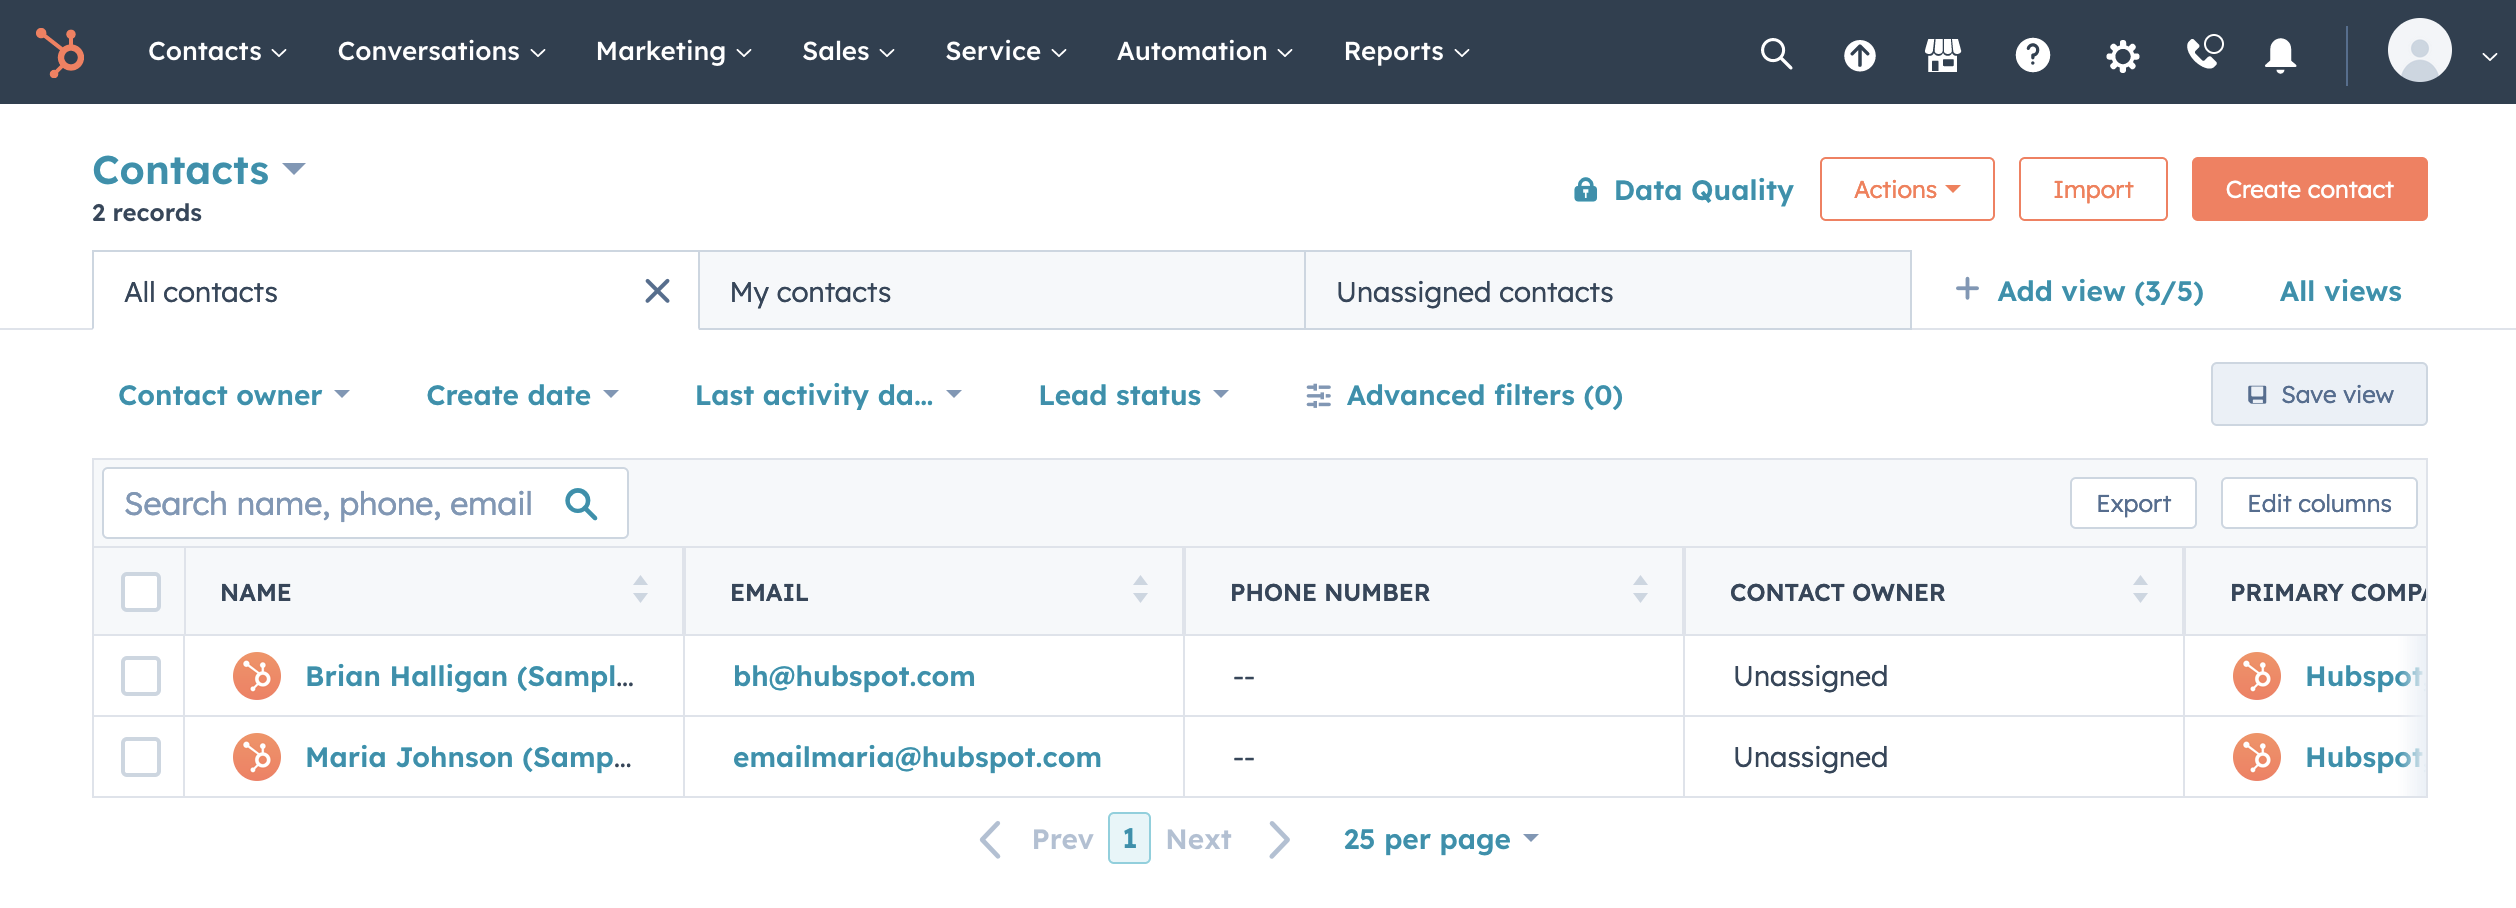
\includegraphics[width=\linewidth]{hubspot.png}}
    \caption{HubSpot customer management panel}
    \label{fig:hubspot}
\end{figure}

They both support handling customer data and tracking purchases. However, HubSpot better visualises this data by providing a more customisable, modular dashboard. On the other hand, Invoice Ninja allows for easier data entry and lookup through their simple interface.

\begin{figure}[ht!]
    \centerline{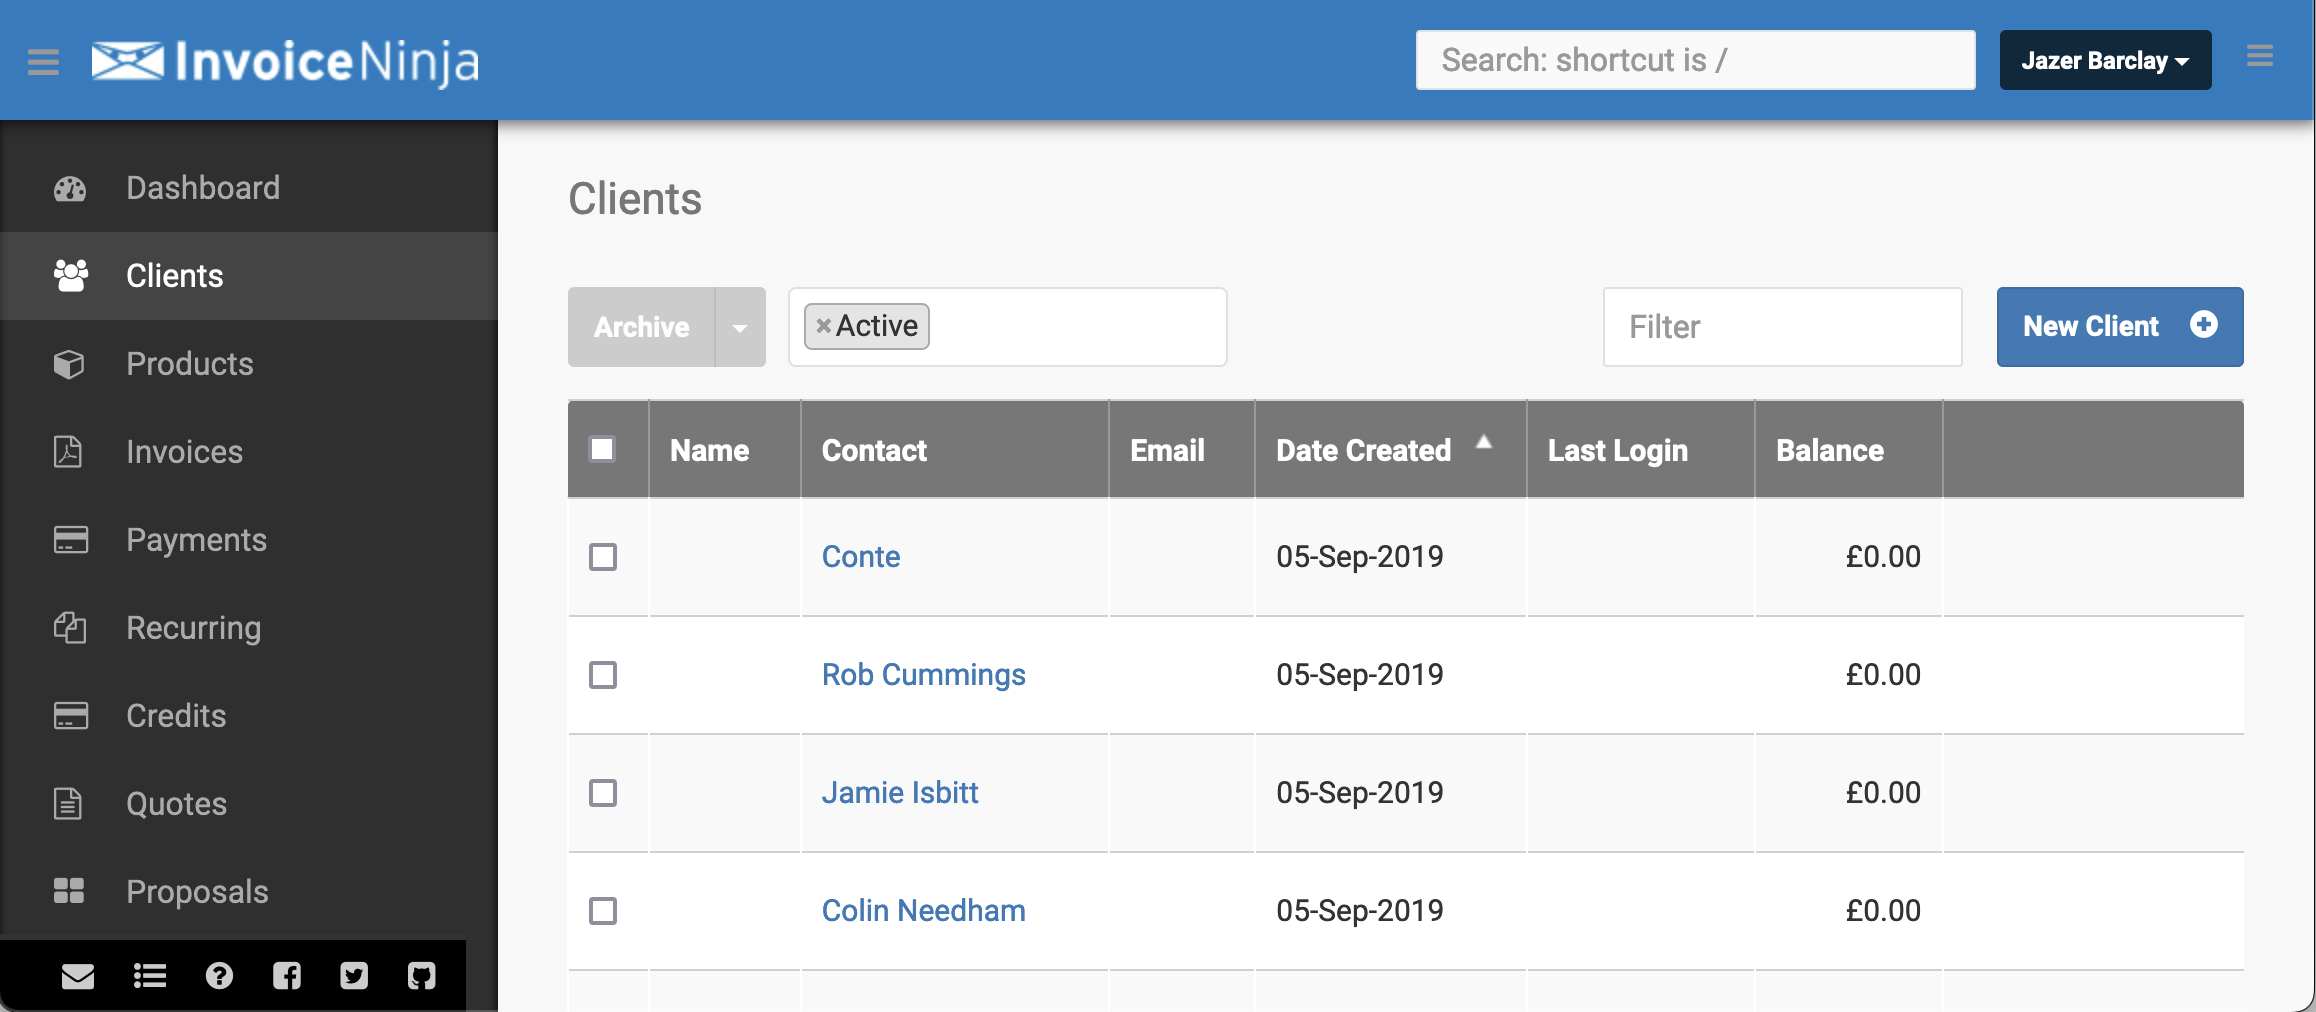
\includegraphics[width=\linewidth]{invoiceninja-customers.png}}
    \caption{Invoice Ninja customer management panel}
    \label{fig:invoiceninja}
\end{figure}

Invoice Ninja meets many more requirements than HubSpot, especially those the business requires, such as efficiently handling customer data entry and lookup. It also supports various products and services, which can be billed as an invoice or purchase.

Where both of these disappoint are in the pricing and lesson purchase models. Neither supports more complex purchase tracking or pricing, which the business needs to prevent further financial losses.

In summary, both software systems provide only some of the system requirements. Nonetheless, no single software covers them all, and neither solves the core issue that the business faces, which involves attendance and payment tracking. Since the primary off-the-shelf software cannot satisfy the requirements, the solution to their problems is within a custom and bespoke system. % Literature Research
%----------------------------------------------------------------------------------------
%	Methodology
%----------------------------------------------------------------------------------------
\chapter{Methodology} % Main chapter title
\label{Chapter3} % For referencing the chapter elsewhere, use \ref{Chapter3}

This chapter covers the development approach employed during development and the software tools used.

%----------------------------------------------------------------------------------------
%	1. Development tools
%----------------------------------------------------------------------------------------

\section{Development tools}
When undertaking any work, using the right tool for the job will improve efficiency, reduce errors and decrease the repetitiveness of tasks. Therefore, the tools used to create this software artefact were carefully selected for their suitability for the project based on their features.

\subsection{Operating System -- MacOS}
An operating system provides the foundation which all other software lives upon. The choice of operating system determines the software tools available and support for specific workflows.

\begin{figure}[ht!]
    \centerline{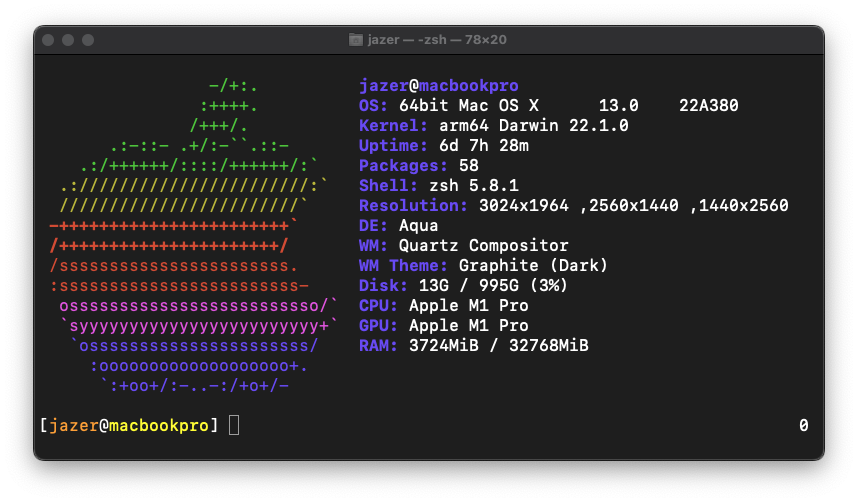
\includegraphics[width=\linewidth]{macos-screenshot.png}}
    \caption{Screenshot of MacOS computer statistics used in development}
    \label{fig:macos}
\end{figure}

MacOS (Figure~\ref{fig:macos}) was the primary choice with its native UNIX command line support for operations \parencite{robbins_unix_2006} and ease of use. This capability helped when running build, test and deployment scripts. Windows also provide this through the Windows Subsystem for Linux \parencite{ionescu_alternatives_2019}; however, it is more complex to set up and interface with Windows applications increasing development time.

In addition to this, MacOS natively supports the Safari browser, which is one of the primary browsers in public use. This support is essential during testing alongside other popular browsers available.


\subsection{Editor - Visual Studio Code}
With the project consisting of three parts, an editor supporting the multiple languages in use and providing methods of operating each is an essential requirement. 

\begin{figure}[ht!]
    \centerline{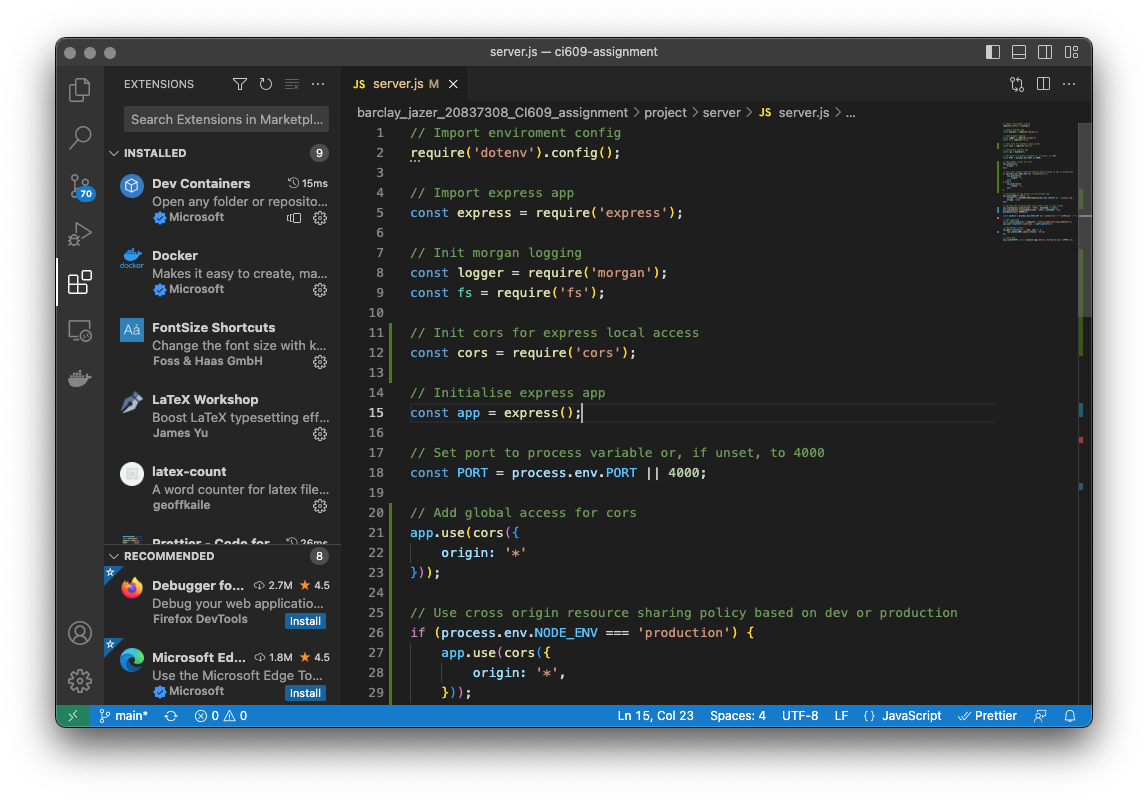
\includegraphics[width=1.1\linewidth]{vscode-screenshot.png}}
    \caption{Screenshot of Visual Studio Code Editor}
    \label{fig:vscode}
\end{figure}

For this reason, Visual Studio Code (Figure~\ref{fig:vscode}) was selected. It is free and provides terminal access from within the development environment to run each part of the project. It also has extensions for syntax highlighting and IntelliSense for each language, reducing development time looking for language specifications or documentation.

Other editors were considered, such as Notepad++, Atom and Sublime. None of these editors had the same features or support VS Code provided at zero cost.


\subsection{Version Control -- Git and GitHub}
A version control system \parencite{zolkifli_version_2018} provides a historical view of changes made to a project's code and a backup of these changes when stored remotely. It enables developers to make experimental changes on new branches without affecting the functional code in a core branch.

\begin{figure}[ht!]
    \centerline{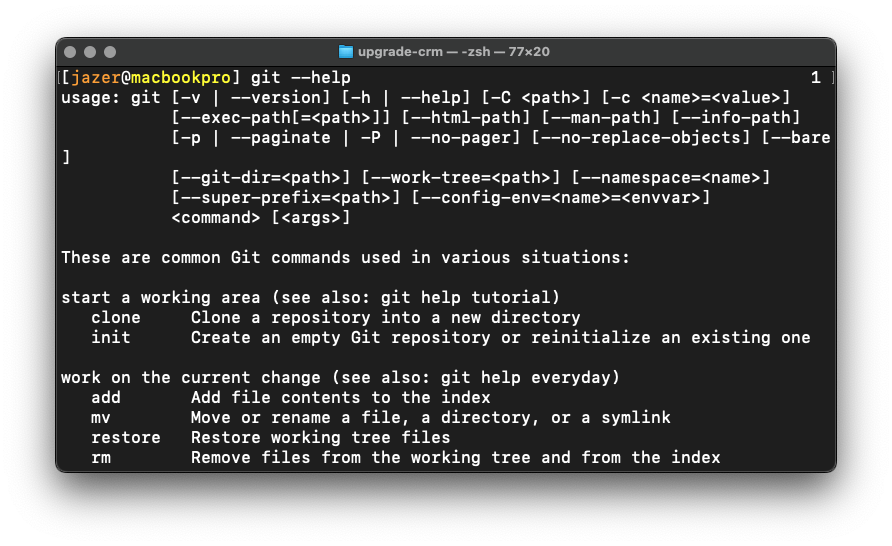
\includegraphics[width=.8\linewidth]{git.png}}
    \caption{Screenshot of Git Help Output}
    \label{fig:git}
\end{figure}

Git \parencite{chacon_pro_2014} was selected for its local and remote storage capabilities (Figure~\ref{fig:git}). It came pre-installed with the operating system as a command line tool. It had a vital role in creating local test branches, which were rebased and merged into the main committed branch.

\begin{figure}[ht!]
    \centerline{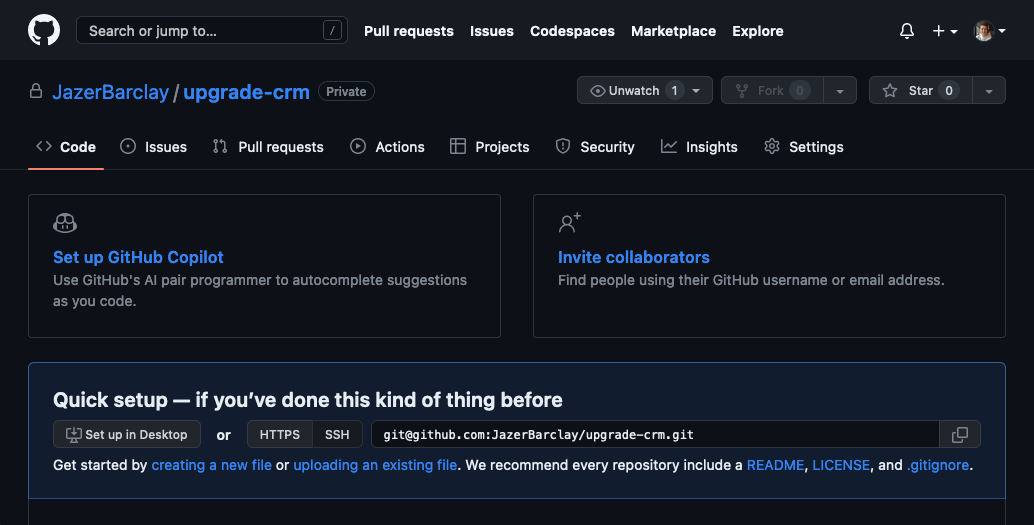
\includegraphics[width=\linewidth]{github.png}}
    \caption{Screenshot of GitHub repository when intialised}
    \label{fig:github}
\end{figure}

GitHub was used with Git \parencite{tsitoara_beginning_2020} to upload the project to the internet (Figure~\ref{fig:github}). This allowed the download of the project to other devices for testing and provided resiliency in the event of a system failure. GitHub also added value through workflows which automated testing when code was uploaded.

Other version control systems, such as SVN \parencite{pilato_version_2008}, were considered for this project but needed more essential features, which Git already provided. In the case of SVN, there is no local history storage, thus requiring an internet connection and online server to track changes. In addition, all history would be lost if the online copy were corrupted or lost.

Other free online Git hosting services exist, such as GitLab, which provides self-hosting options but does not have the same ease of use that Github provides.


\subsection{Web Browser -- Firefox}
Web-based projects require a browser for viewing and testing. Although many were used in the project's testing phase, one was selected for use during development.

\begin{figure}[ht!]
    \centerline{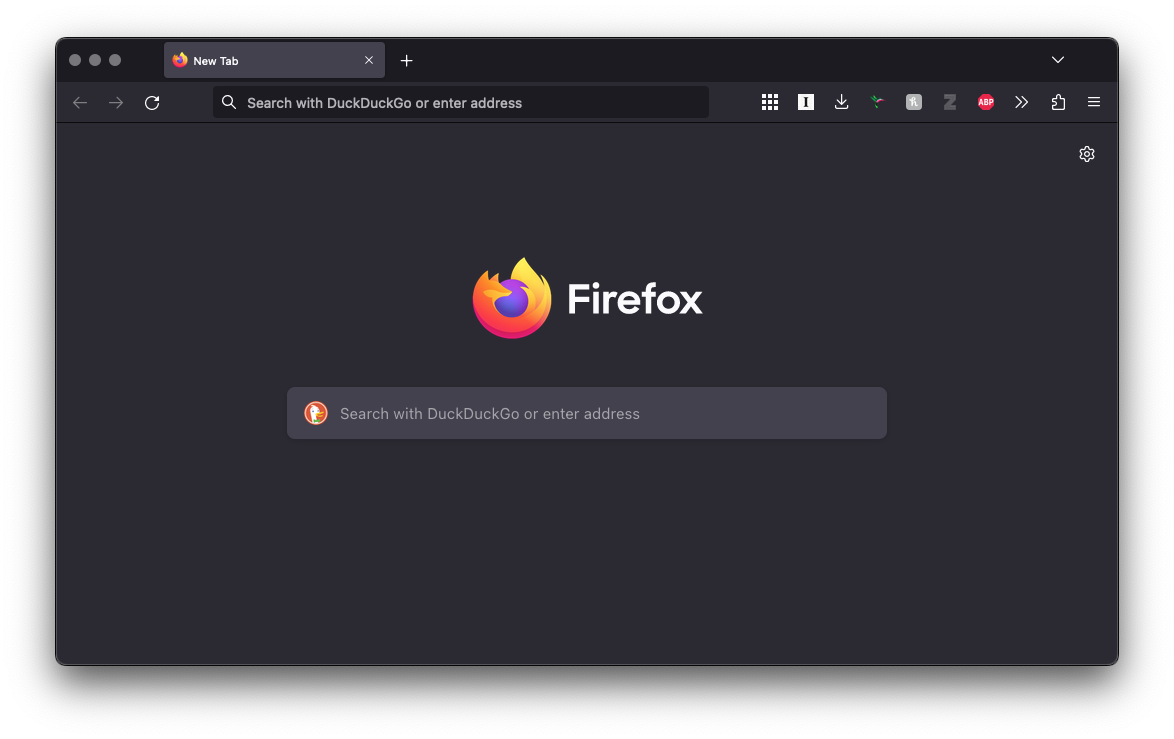
\includegraphics[width=1.1\linewidth]{firefox.png}}
    \caption{Screenshot of the Firefox Web Browser}
    \label{fig:firefox}
\end{figure}

Firefox (Figure~\ref{fig:firefox}) was primarily used with its feature-rich developer support providing a built-in console, page layout viewer and view of local storage variables. Other browsers were later used for testing to ensure the system functions across all, including Google Chrome, Safari, Opera and Microsoft Edge.


\subsection{API Interaction -- Postman}
An API was used to interface with the database. The web browser can interact with the API, albeit crudely and with limited functionality.

\begin{figure}[ht!]
    \centerline{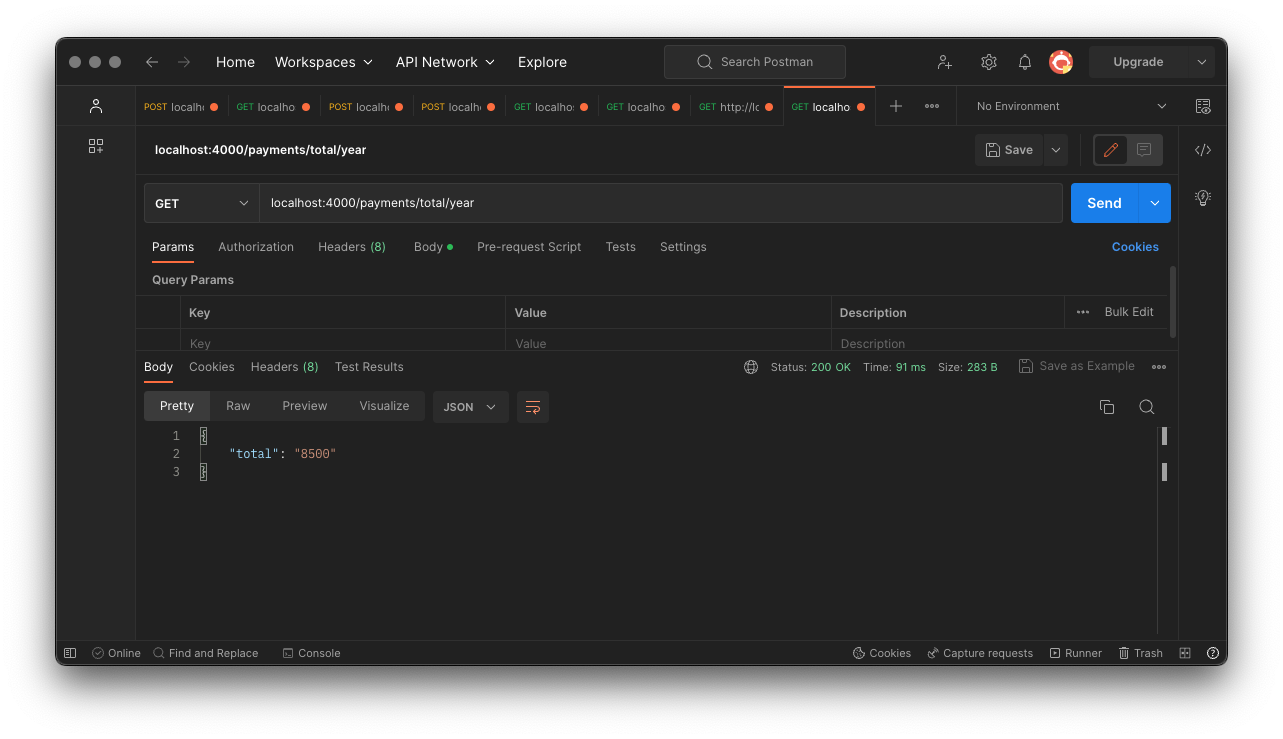
\includegraphics[width=.9\linewidth]{postman.png}}
    \caption{Screenshot of the Postman API Tool}
    \label{fig:postman}
\end{figure}

Postman (Figure~\ref{fig:postman}) was utilised for crafting custom API requests and automated black box testing requests for edge and error cases to aid in the development and testing of the API.


\subsection{Database Management System -- PostgreSQL}
A database management system allows direct access and manipulation of data stored in a database without requiring a recompilation. This access is valuable during development for quick modifications, testing data storage types and links between tables.

\begin{figure}[ht!]
    \centerline{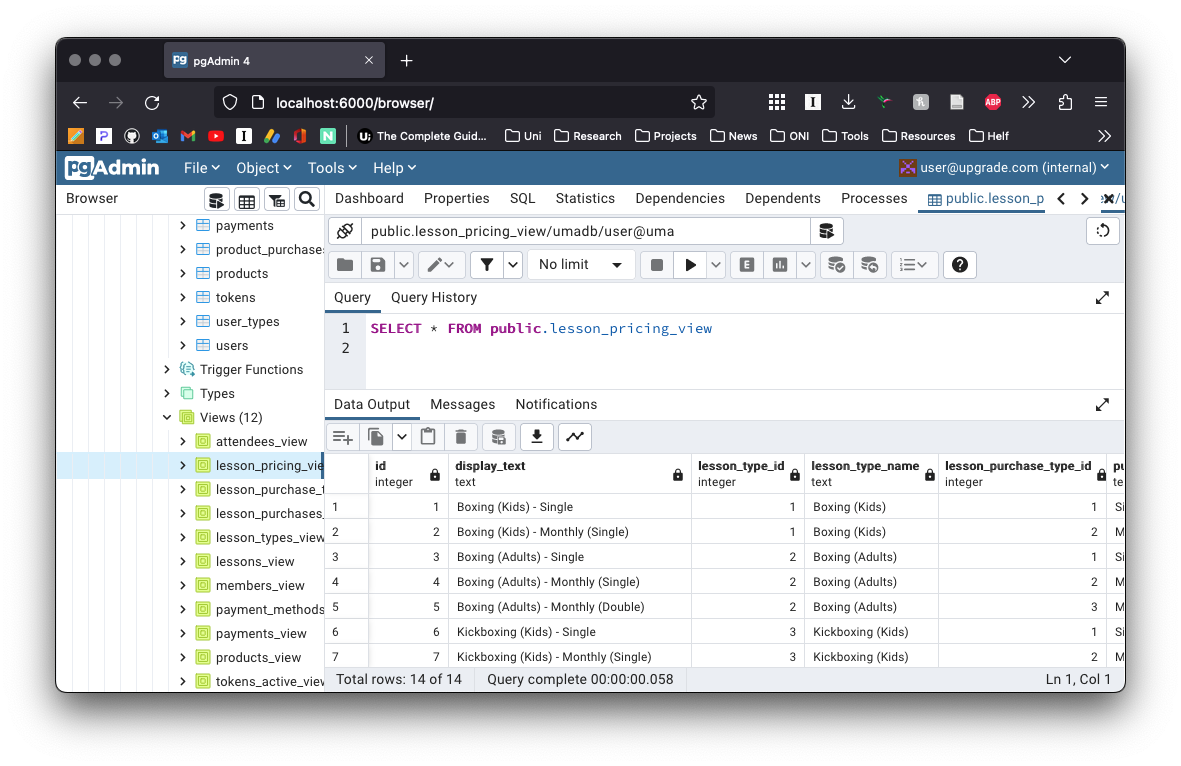
\includegraphics[width=.9\linewidth]{pgadmin.png}}
    \caption{Screenshot of PgAdmin4 Interface for Accessing the Database}
    \label{fig:pgadmin}
\end{figure}

With PostgreSQL within Docker providing the database for this project, the PgAdmin4 tool (Figure~\ref{fig:pgadmin}) was utilised within the same Docker environment. PgAdmin includes analytics to the PostgreSQL database and table creation and modification tools.

Other tools exist to interface with a database however are very generic and designed to operate with any relational database.


\subsection{Deployment - Docker}
Docker (Figure~\ref{fig:docker}) standardised testing and deployment environments to contain each project segment through the use of containers \parencite{merkel_docker_2014}. Each component could be tested individually for errors and rebuilt for deployment on the development or live server when changes were made.

\begin{figure}[ht!]
    \centerline{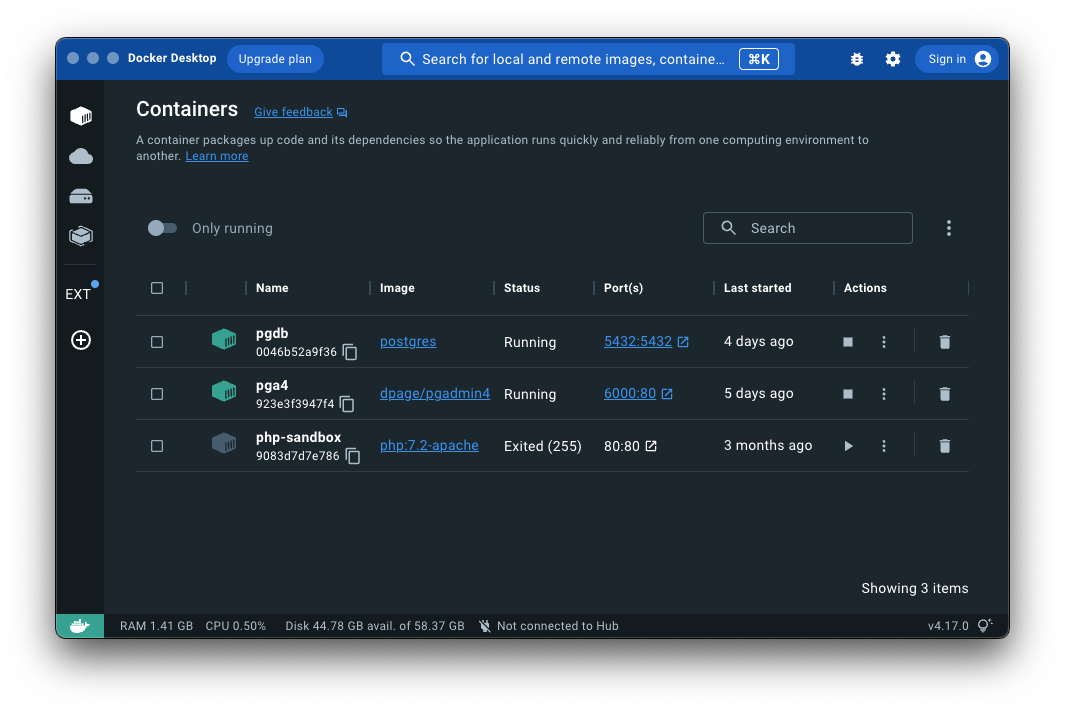
\includegraphics[width=1.1\linewidth]{docker.png}}
    \caption{Screenshot of the Docker Dashboard with Running Containers}
    \label{fig:docker}
\end{figure}

\subsection{Project Tracking -- Trello}
Maintaining progress through the project lifecycle is vital to remain on track and within the time constraints. The software must be flexible to fit the developer's approach while remaining uncomplicated.

\begin{figure}[ht!]
    \centerline{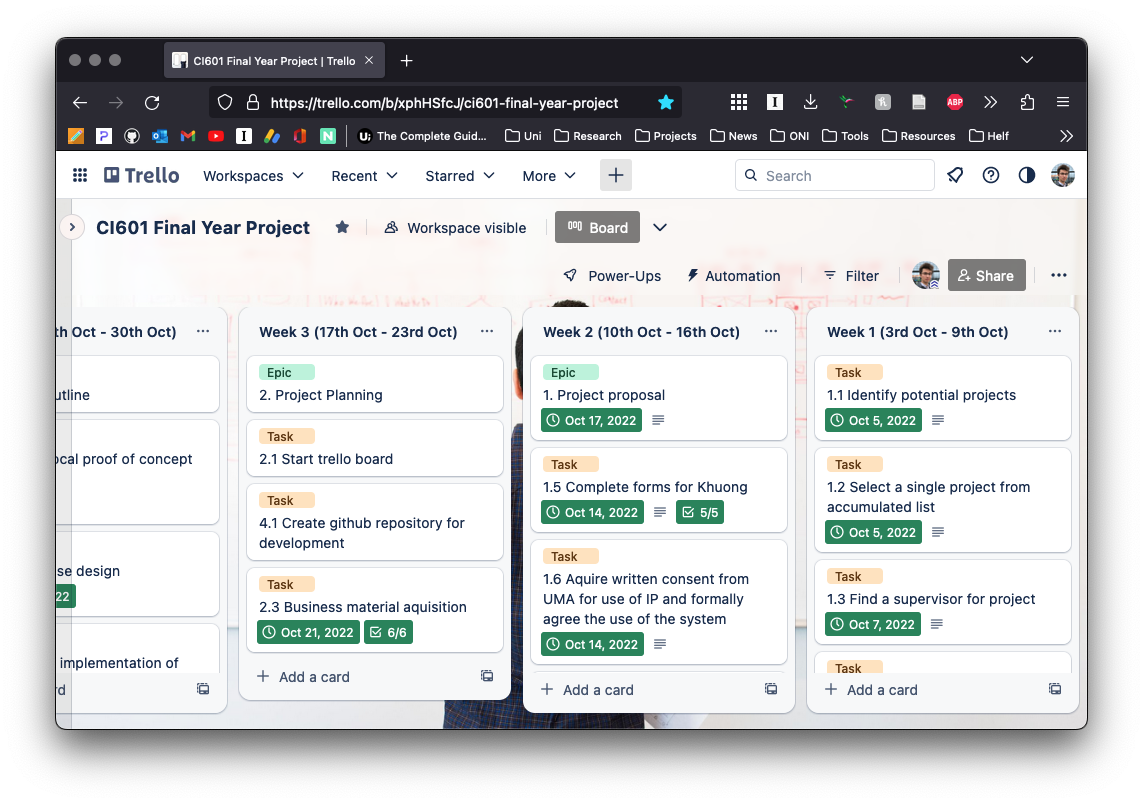
\includegraphics[width=1.1\linewidth]{trello.png}}
    \caption{Screenshot of Trello Running in Firefox}
    \label{fig:trello}
\end{figure}

Trello (Figure~\ref{fig:trello}) was selected to track the project's progress from inception to creation. It is an online Kanban board system designed to support lists and cards. Having a visual display of the features to be added, the current work in progress, and what has been completed each week provides great insight helping with time estimates with work and keeping work only to the tasks which move the project closer to its goals.

Atlassian also provided a tool designed specifically for agile and the scrum approach. However, it was more complicated and geared towards collaboration rather than simple project management.


%----------------------------------------------------------------------------------------
%	2. Development approach
%----------------------------------------------------------------------------------------

\section{Development approach}
There are many approaches developers and businesses may use to structure software development, each with its benefits and drawbacks. With this project being a solo endeavour, a system primarily focused on collaboration would be less beneficial than one designed to deliver features.

Since this project has a short timeframe and an end date, non-iterative approaches such as the waterfall method (Figure~\ref{fig:water}) would be unproductive \parencite{mpcs_waterfall_2012}. Feedback from the business owners and supervisor, including bug fixes and edge cases, would not be actionable and require a new development stint beyond the project's deadline.

\begin{figure}[ht!]
    \centerline{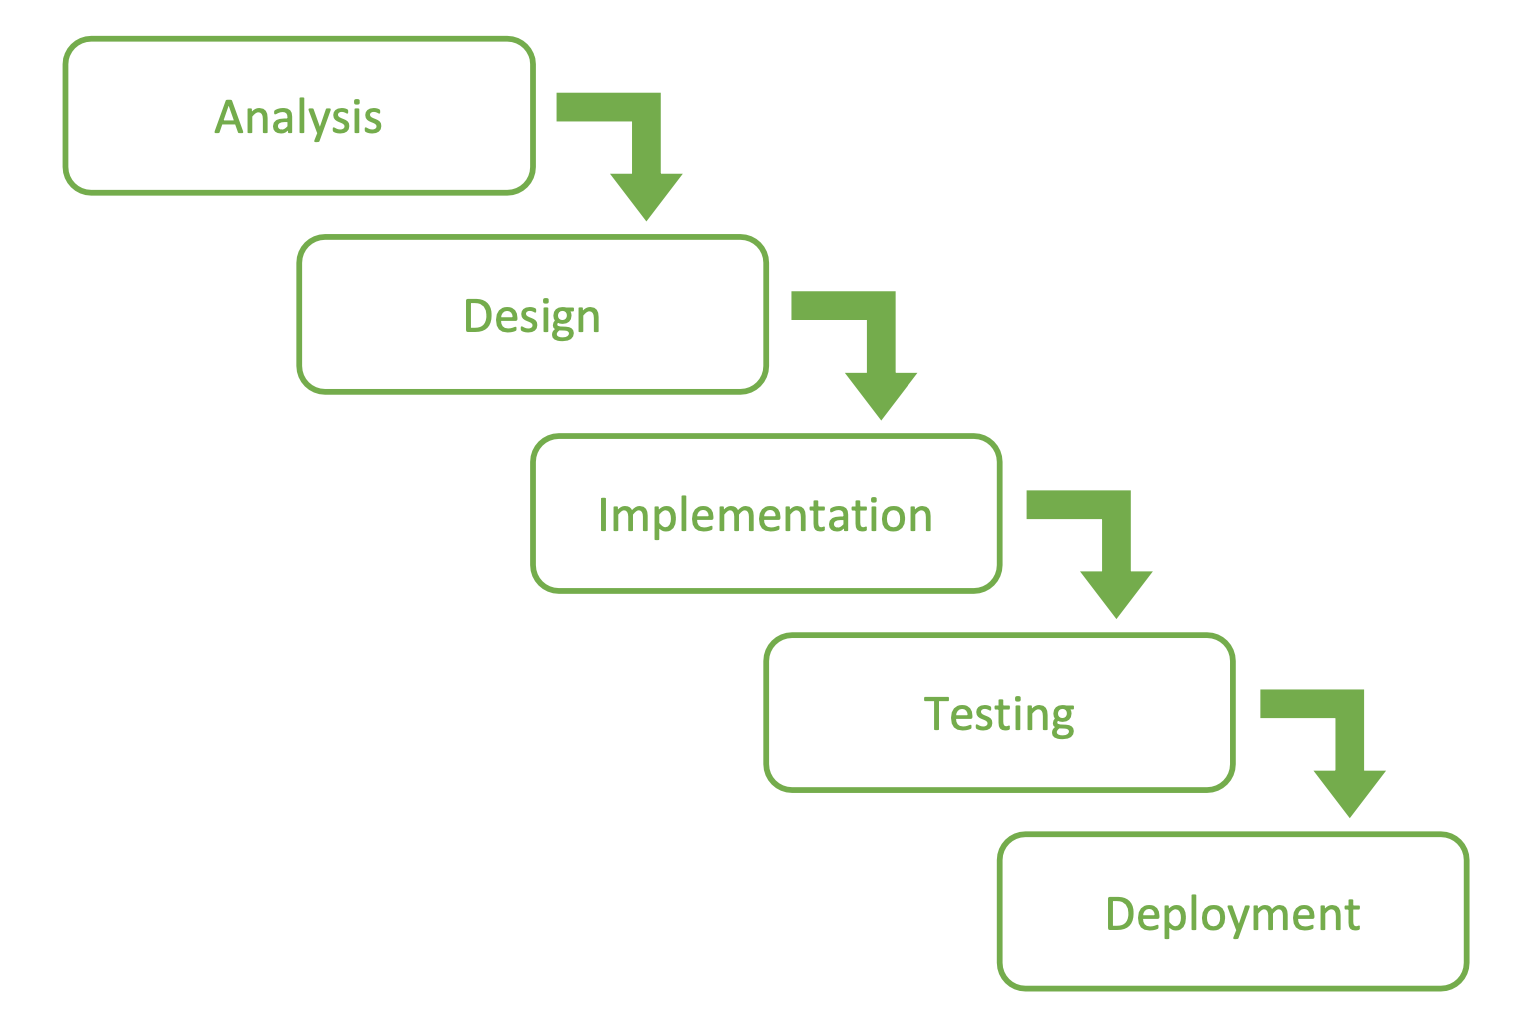
\includegraphics[width=.9\linewidth]{waterfall.png}}
    \caption{The Waterfall Development Method}
    \label{fig:water}
\end{figure}

Agile \parencite{shore_art_2022} (Figure~\ref{fig:agile}) and Feature Driven Development (FDD) (Figure~\ref{fig:fdd}) were the two promising strategies for this project. The agile approach is designed more for teams however emphasises regular meetings with stakeholders and project managers. FDD, on the other hand, is about delivering features in a more structured manner with less focus on a team \parencite{lucid_why_2019}.


\begin{figure}[h!]
    \centerline{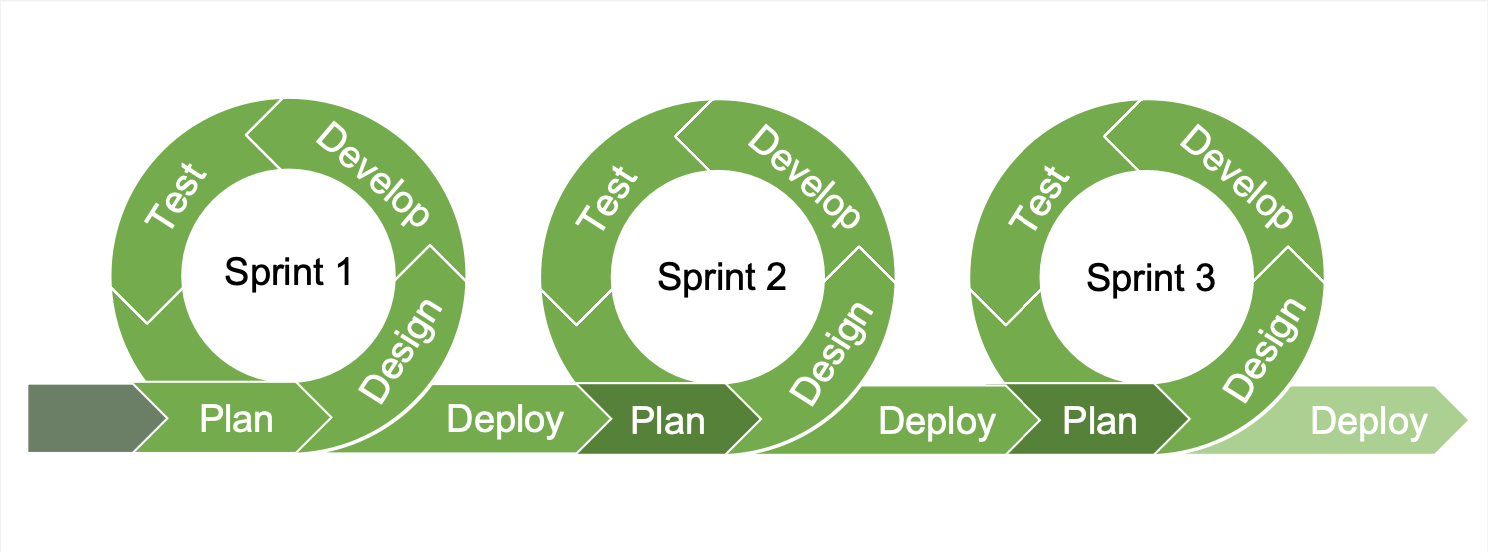
\includegraphics[width=1.1\linewidth]{agile.png}}
    \caption{The Agile Iterative Development Method}
    \label{fig:agile}
\end{figure}

\begin{figure}[h!]
    \centerline{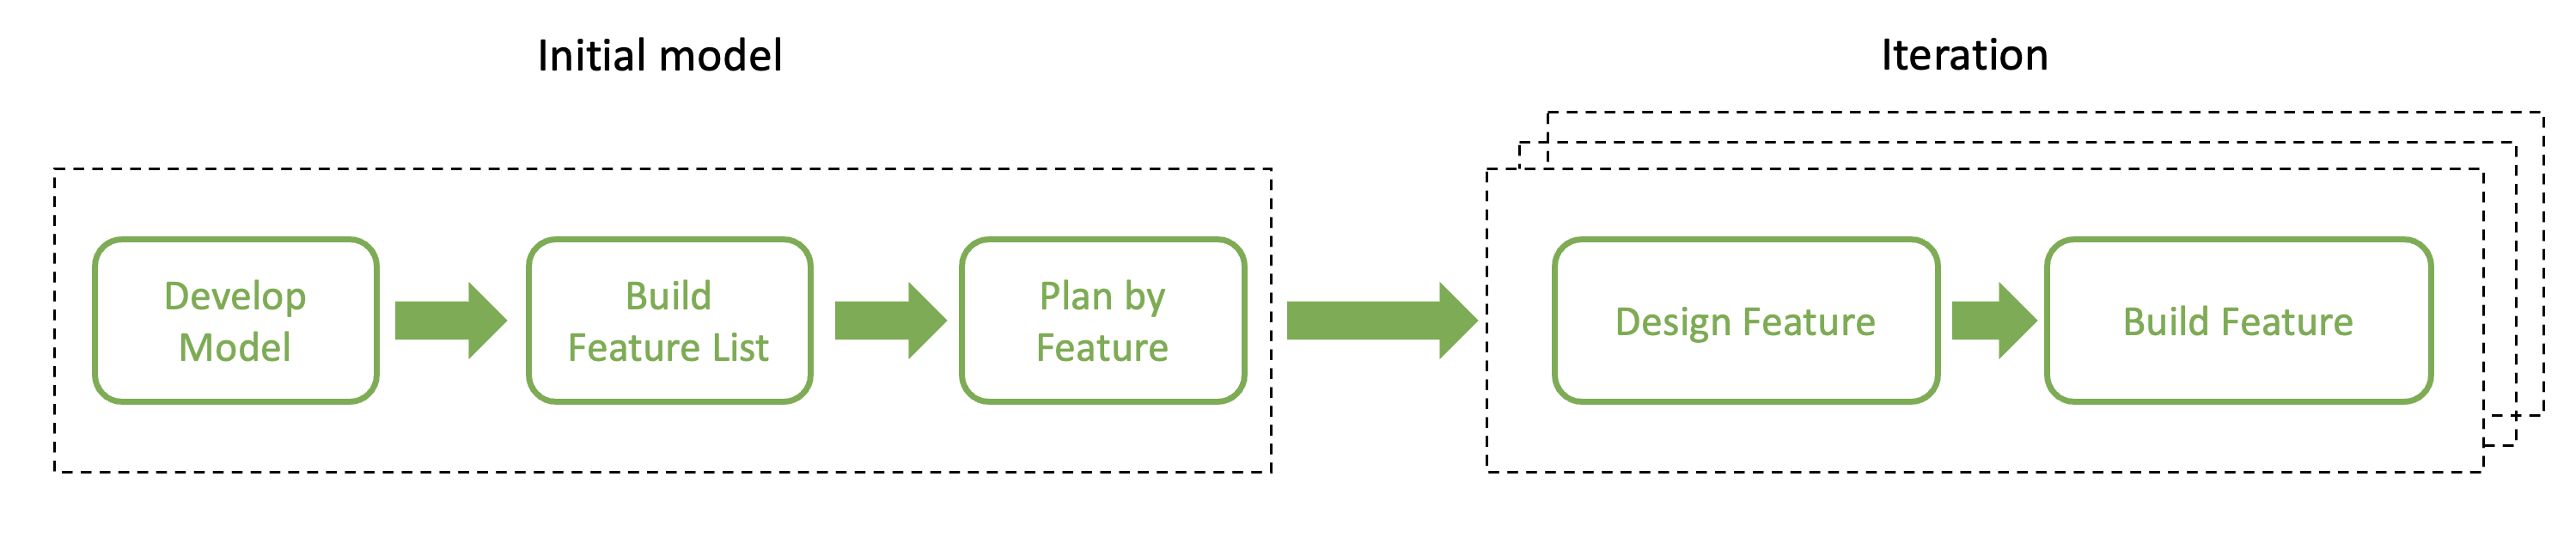
\includegraphics[width=1.1\linewidth]{fdd.png}}
    \caption{The Feature-Driven Development Method}
    \label{fig:fdd}
\end{figure}

Both provided certain qualities that the project development structure would require. However, no specific structure or approach is set in stone; As a result, a mixture of both was employed \parencite{sremath_tirumala_hybrid_2016}. Agile qualities, including sprints, regular check-ins with the supervisor and business managers, and a feature delivery focus structure from FDD, were ultimately used when building the software.

This structure can be seen in the Gantt charts (Figures~\ref{fig:gantt1} and~\ref{fig:gantt2}) created at the beginning of the project, splitting work into an initial development stage before the winter break and bi-weekly sprints where new features are added for greater functionality.

\begin{figure}[ht!]
    \centerline{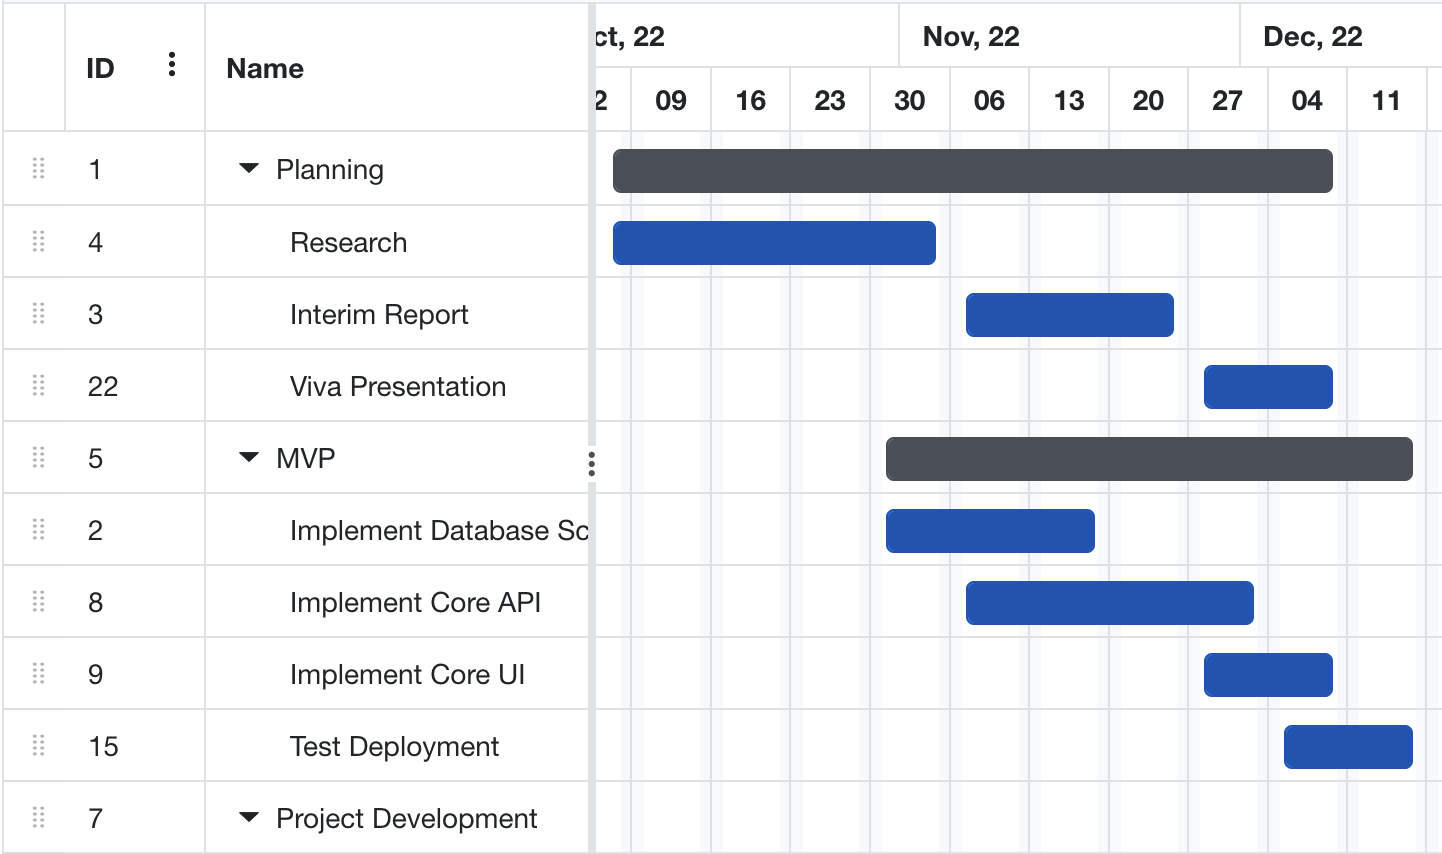
\includegraphics[width=1\linewidth]{gantt1.png}}
    \caption{A Gantt Chart of the planning phase of this Project}
    \label{fig:gantt1}
\end{figure}

\begin{figure}[ht!]
    \centerline{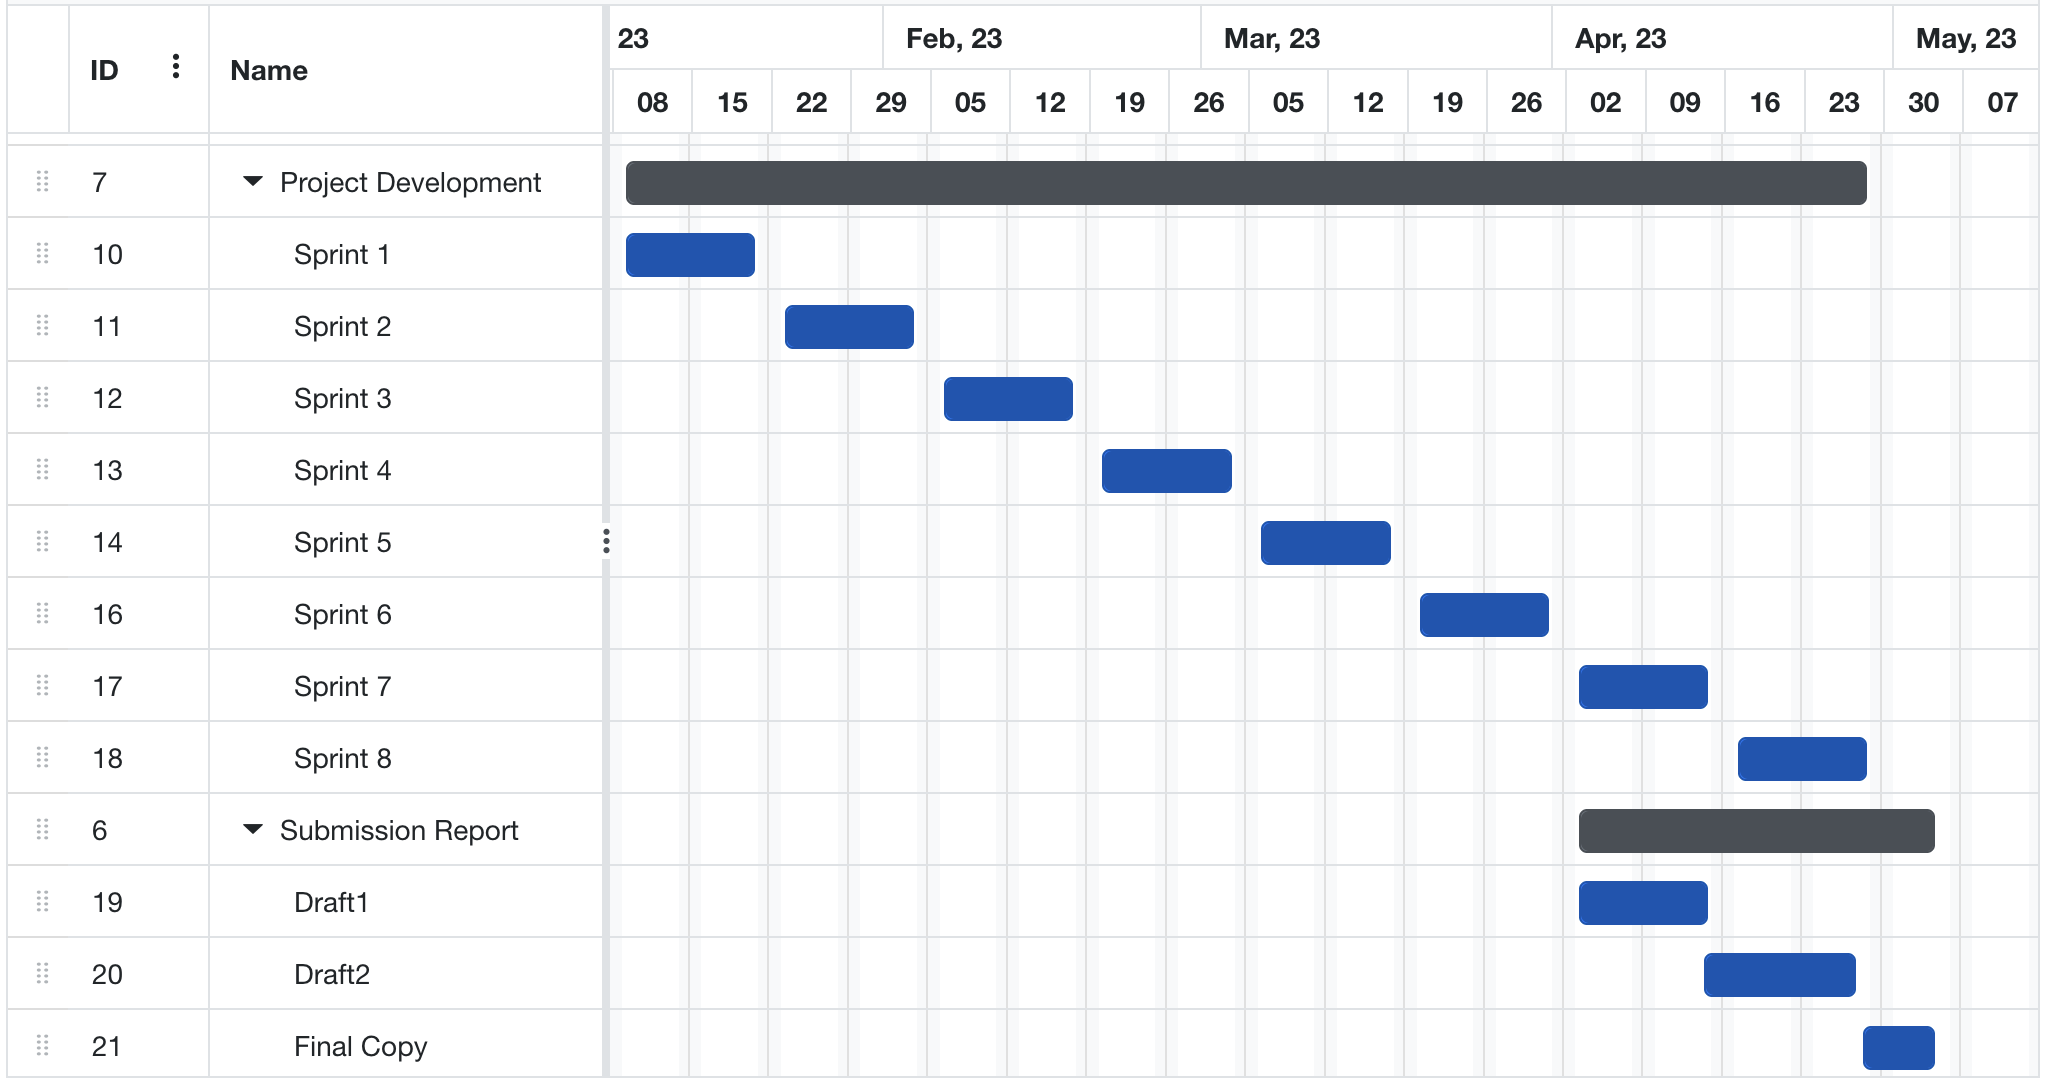
\includegraphics[width=1\linewidth]{gantt2.png}}
    \caption{A Gantt Chart of the sprint development phase of this Project}
    \label{fig:gantt2}
\end{figure}

A further breakdown of the work completed in the initial stages and the bi-weekly sprints is available through the tracked progress in Trello.

\begin{figure}[ht!]
    \centerline{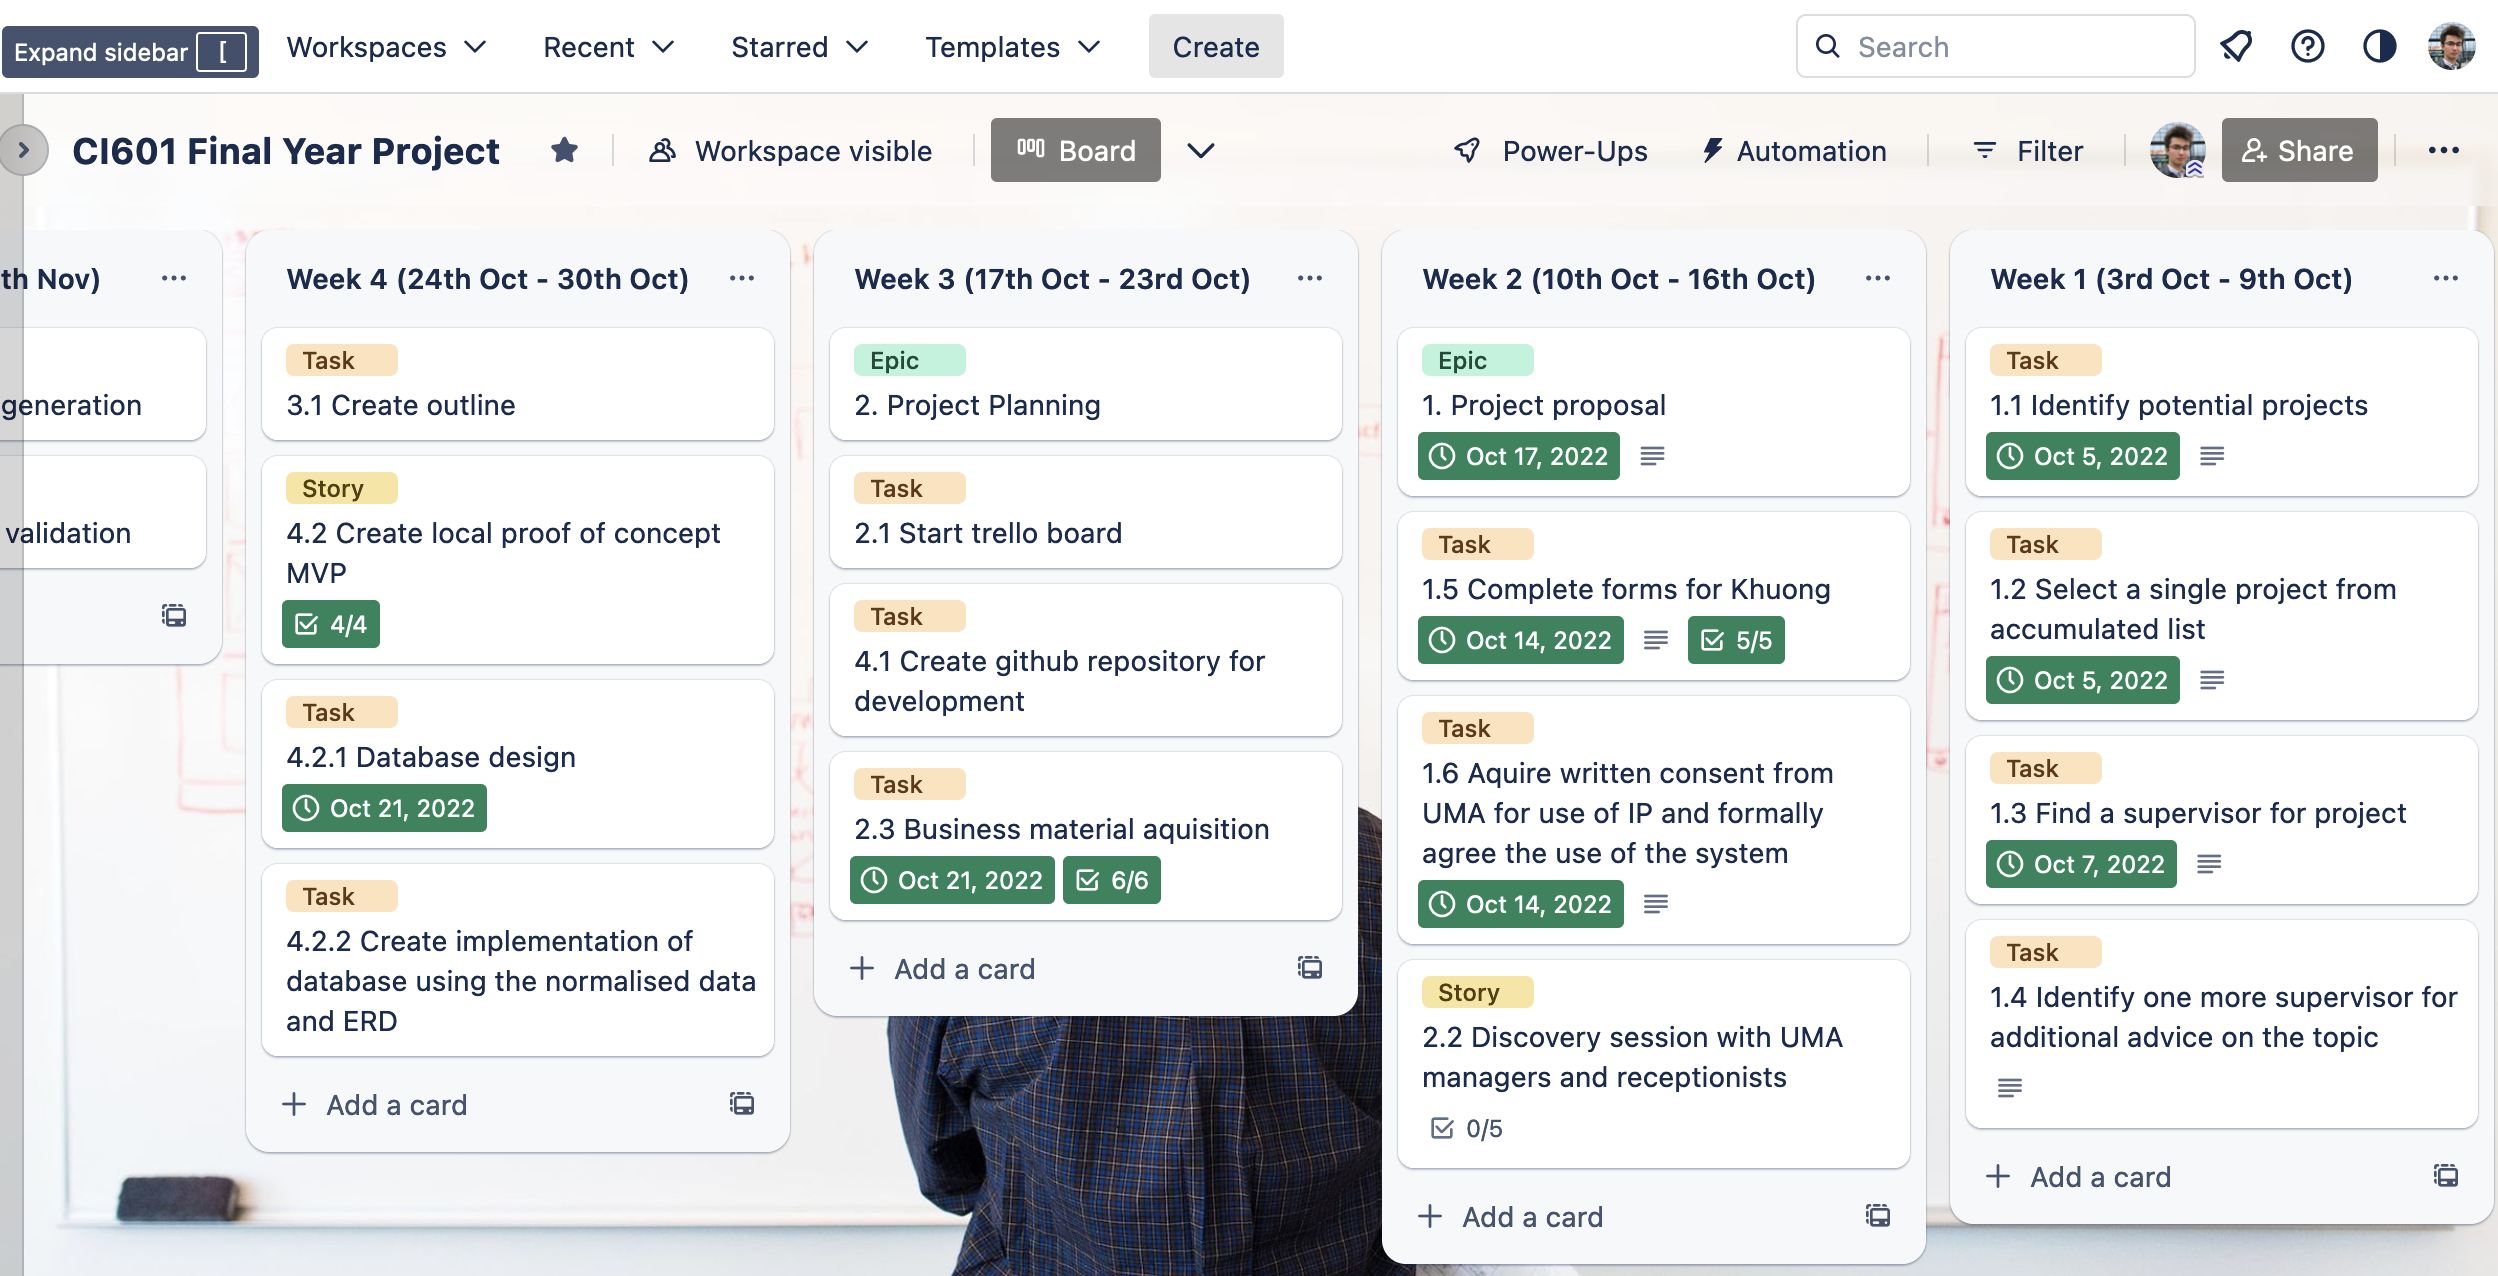
\includegraphics[width=1\linewidth]{trello-first.png}}
    \caption{Screenshot of First 4 Weeks Tracked on Trello}
    \label{fig:trello-board}
\end{figure} % Methodology
%----------------------------------------------------------------------------------------
%	Product description
%----------------------------------------------------------------------------------------
\chapter{Product description} % Main chapter title
\label{Chapter4} % For referencing the chapter elsewhere, use \ref{Chapter4}
This chapter covers the system's design, starting with the complete system architecture and then going into each component in greater detail.


%----------------------------------------------------------------------------------------
%	1. System requirements
%----------------------------------------------------------------------------------------

\section{System requirements}
Initial discovery sessions with the business owners, managers, and receptionists uncovered the requirements for the system and their use cases. These requirements can be split into four types \parencite{cox_business_2021}: business, user, functional and quality.

Business requirements are what the business wants to achieve (Figure~\ref{fig:businessreq}). These are the overall objectives which the project aims to address.

The user requirements are what the user requires the system to provide to achieve the business requirements (Figure~\ref{fig:userreq}). These provide insight into the user stories and support the functional requirements.

Functional requirements describe the software's activities and processes to achieve the user requirements (Figure~\ref{fig:functionalreq}). These are the functions which the system must support that tie into the user requirements.

Quality requirements describe the performance and metrics the functional requirements within the system must achieve(Figure~\ref{fig:qualityreq}).

\begin{table}[ht!]
    \caption{Business requirements}
    \renewcommand{\arraystretch}{1.5}
    \centerline{
        \begin{NiceTabular}{ m{1cm} m{9cm} m{2.5cm}  }
            \hline
            \textbf{ID} & \textbf{Requirement} & \textbf{Priority}\\
            \hline \hline
            BR1 & A system which is accessible within the gym and off-site (residence). The system must be online & Must have\\
            \hline
            BR2 & Multi-device support to view and edit data & Must have\\
            \hline
            BR3 & Unify method of data search and entry & Must have\\
            \hline
            BR4 & Reduce input and search time on data by at least 50\% & Must have\\
            \hline
            BR5 & Increase profit by removing non-payment attendance & Should have\\
            \hline
            BR6 & Provide insights to improve business-making decisions & Should have\\
            \hline
           \end{NiceTabular}
    }
    \label{fig:businessreq}
\end{table}

\ \\

\begin{table}[ht!]
    \caption{User requirements}
    \renewcommand{\arraystretch}{1.5}
    \centerline{
        \begin{NiceTabular}{ m{1cm} m{9cm} m{2.5cm}  }
            \hline
            ID & Requirement & Priority\\
            \hline \hline
            UR1 & Staff must log in to prevent unauthorised access. (Since the system will be available online). The system must be online & Must have\\
            \hline
            UR2 & Staff can input, view and edit member data. (Needed for adding new members and supporting existing customers) & Must have\\
            \hline
            UR3 & Add and edit lessons available for each day. (Lessons must also be tracked for attendance) & Must have\\
            \hline
            UR4 & The receptionist can add members to lessons. (Attendance must be tracked) & Must have\\
            \hline
            UR5 & The receptionist can take payments which correlate to available attendance to lessons. (Lesson type and purchase type length at play) & Must have\\
            \hline
            UR6 & Provide metrics on business performance (member signup, attendance, payment totals) across a date range (day, week, month, year) & Must have\\
            \hline
           \end{NiceTabular}
    }
    \label{fig:userreq}
\end{table}

\ \\

\begin{table}[ht!]
    \caption{Functional requirements}
    \renewcommand{\arraystretch}{1.5}
    \centerline{
        \begin{NiceTabular}{ m{1cm} m{9cm} m{2.5cm}  }
            \hline
            ID & Requirement & Priority\\
            \hline \hline
            FR1 & Add, view and edit members & Must have\\
            \hline
            FR2 & Add, view and edit lessons & Must have\\
            \hline
            FR3 & Add and view payments & Must have\\
            \hline
            FR4 & Add and view purchases & Must have\\
            \hline
            FR5 & Support bulk-purchase of lessons & Must have\\
            \hline
            FR6 & Handle member attendances for lessons based on purchases & Must have\\
            \hline
            FR7 & Provide member, attendance and payment statistics over day, week, month and fiscal year & Should have\\
            \hline
           \end{NiceTabular}
    }
    \label{fig:functionalreq}
\end{table}

\ \\

\begin{table}[ht!]
    \caption{Quality requirements}
    \renewcommand{\arraystretch}{1.5}
    \centerline{
        \begin{NiceTabular}{ m{1cm} m{9cm} m{2.5cm}  }
            \hline
            ID & Requirement & Priority\\
            \hline \hline
            QR1 & Reduce member search time to less than 30 seconds & Must have\\
            \hline
            QR2 & Reduce accounting time by at least half for payments & Should have\\
            \hline
           \end{NiceTabular}
    }
    \label{fig:qualityreq}
\end{table}

\section{Problem solving}
Supporting the user experience while accurately storing the data was lengthy and complex. However, the most complex was solving the issue of lesson bulk-purchase tracking in tandem with attendance.

Were this for single lessons, the purchase could be linked to the attendance making for an outer join solve the problem. However, this would not work since a single purchase could constitute a collection of lessons.

Another solution would be to recalculate upon each attendance request. Each attendance request would count up the total number of lessons remaining by adding up valid payments, deducting past attendances, and finally returning the total number of lessons remaining. This would work, yet it results in longer wait times for receptionists tracking attendance. In addition, as the database grows, the wait time will also grow at an exponential rate.

The solution selected was to create tokens. Lesson purchases will generate tokens allowing access only if tokens are available for the requested lesson. Single lessons generate a token for that type of lesson that lasts seven days (Figure~\ref{fig:single-token}). This solution works similarly to the original idea.

\begin{figure}[ht!]
    \centerline{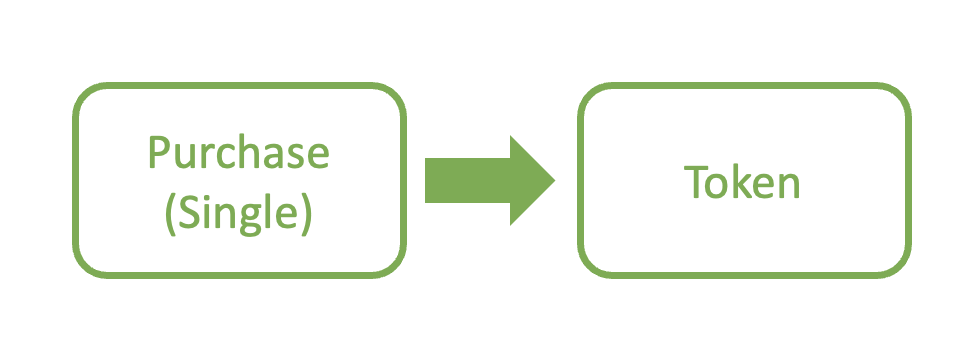
\includegraphics[width=0.5\linewidth]{single-purchase-token.png}}
    \caption{Token generation from single lesson purchase}
    \label{fig:single-token}
\end{figure}

Depending on the lesson type (monthly single, monthly double, etc.), bulk purchases will generate a different quantity of tokens based on the purchase type. This adds a heavier load to when a purchase is made but can be completed quickly since additions are linear, whereas searches are slower when calculating across linked tables.

\begin{figure}[ht!]
    \centerline{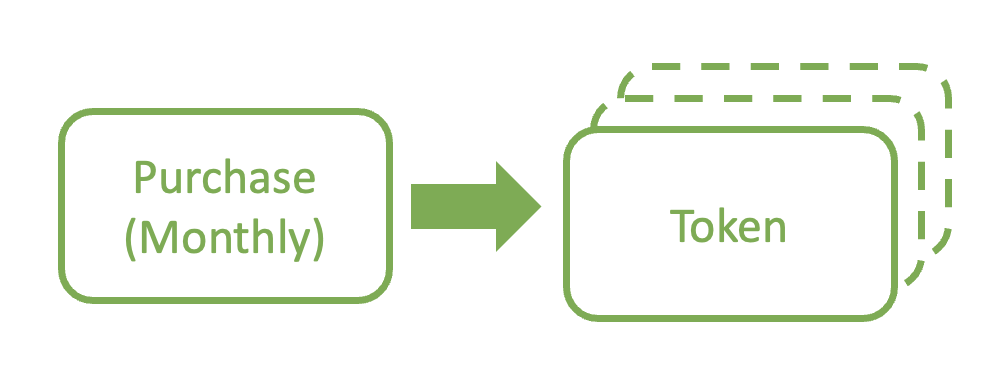
\includegraphics[width=0.5\linewidth]{monthly-purchase-tokens.png}}
    \caption{Multiple tokens generated from monthly lesson purchase}
    \label{fig:multi-token}
\end{figure}

If the member does not have an available valid token, they must either pay now to acquire one for the lesson making for a single lesson purchase or pay later, adding debt to their account.

This solution must be handled within the API and a carefully structured database table to enforce the need for this token for attendance. The correct number and dates must be applied to these tokens to ensure members are not paying and unable to attend due to incorrect validity times. The UI will also need to interact with this, informing the receptionist if the user has a valid token or not.


%----------------------------------------------------------------------------------------
%	2. System architecture
%----------------------------------------------------------------------------------------

\section{System architecture}

\subsection{Software type}
Based on requirement BR1, the data would need to be hosted online in some capacity allowing devices to access a central store of data. For example, this could be through an application or website.

This requirement raised the question of application type. Requirement BR2, which also requires multi-device access, helped narrow the focus to a progressive web application (PWA) \parencite{tandel_impact_2018}.

A desktop application is not portable. Although some languages, such as Java, support running a single compiled binary on many devices, it remains limited to desktop devices. In addition, mobiles and tables would require their native application to be written separately, thus doubling the workload. Likewise, mobile applications would also require a different build for Android and iOS, respectively.

Progressive web applications, and web applications in general, solve this issue. All devices support viewing web application interaction through a browser, and many modern operating systems on desktop and mobile devices support viewing progressive web applications as pseudo-native applications \parencite{biorn-hansen_progressive_2017}. Therefore, these applications can be bookmarked on desktop and mobile devices and behave like native applications.


\subsection{Software structure}
For any application, data storage and system interaction are vital components which must be considered. Combined with the complexity of their pricing and attendance requirements, a logical layer that ties the interaction and the data storage will help separate concerns. This separation creates a 3-tier architecture \parencite{fernandez_secure_2008} which follows the single responsibility, clean code design principle \parencite{martin_clean_2008}.

\begin{figure}[ht!]
    \centerline{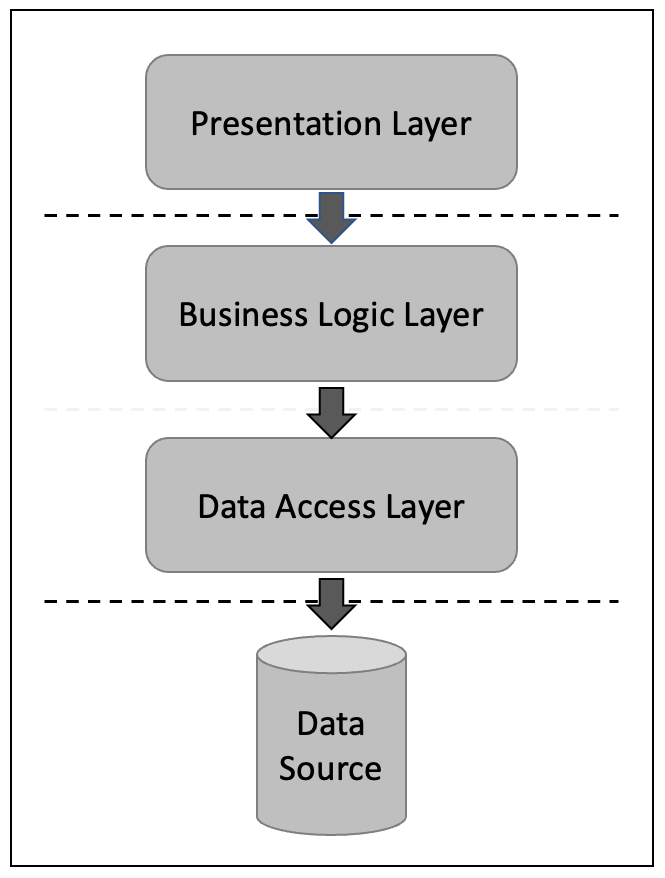
\includegraphics[width=0.5\linewidth]{3-tier.png}}
    \caption{Diagram of the 3-tier system architecture}
    \label{fig:sysarch}
\end{figure}

The three components of this system consist of a data layer, a logic layer and a presentation layer (Figure~\ref{fig:sysarch}). 

The data layer manages data storage and supports data submission, modification, and removal. For this reason, a relational database was selected to handle the storage of member records, attendance and pricing.

The presentation layer expresses the data in a user-friendly manner and handles user input. The display consists of components for displaying the data, such as graphs and elements to add and modify the data, including forms, buttons, text boxes and drop-down menus.

Finally, the logical layer handles the operations that the system can perform. Rather than the presentation layer handling how the database updates the data and sanitising the inputs, the logical layer performs all of the checks, modifies the data layer and provides responses to the presentation layer. This layer provides the functionality and bridge between the data and presentation layer.

This 3-tier design also supports future considerations, such as other front-end applications providing users with new ways of viewing and interacting with the system. It also provides a valuable structure for testing and scalability where each layer can be individually tested for functionality and scaled horizontally if required.


%----------------------------------------------------------------------------------------
%	3. Database design
%----------------------------------------------------------------------------------------

\section{Database design}
Discovery sessions and existing documentation provided the template for what data needs to be stored, including price lists and member signup forms. Normalisation was then applied to streamline the data model \parencite{date_database_2019}.

Normalisation is the process of refining how a relational database will store data to decrease redundancy and improve dependencies while maintaining data integrity. It uses multiple stages which apply a set of rules called 'normal forms'. These optimise the data layout incrementally from the first to the third normal form.

The first normal form minimised redundant data by making all fields atomic. The second normal form splits the data into their respective tables, reducing the repetition of values stored. Finally, the third normal form makes explicit dependencies resolving the many-to-many relationships. These steps combined have improved the consistency of data storage, reduced errors and ensured data integrity.

To better understand the structure for future development, an entity relationship diagram (ERD) was created as part of the documentation for this project (Figure~\ref{fig:erd}).

\begin{figure}[ht!]
    \centerline{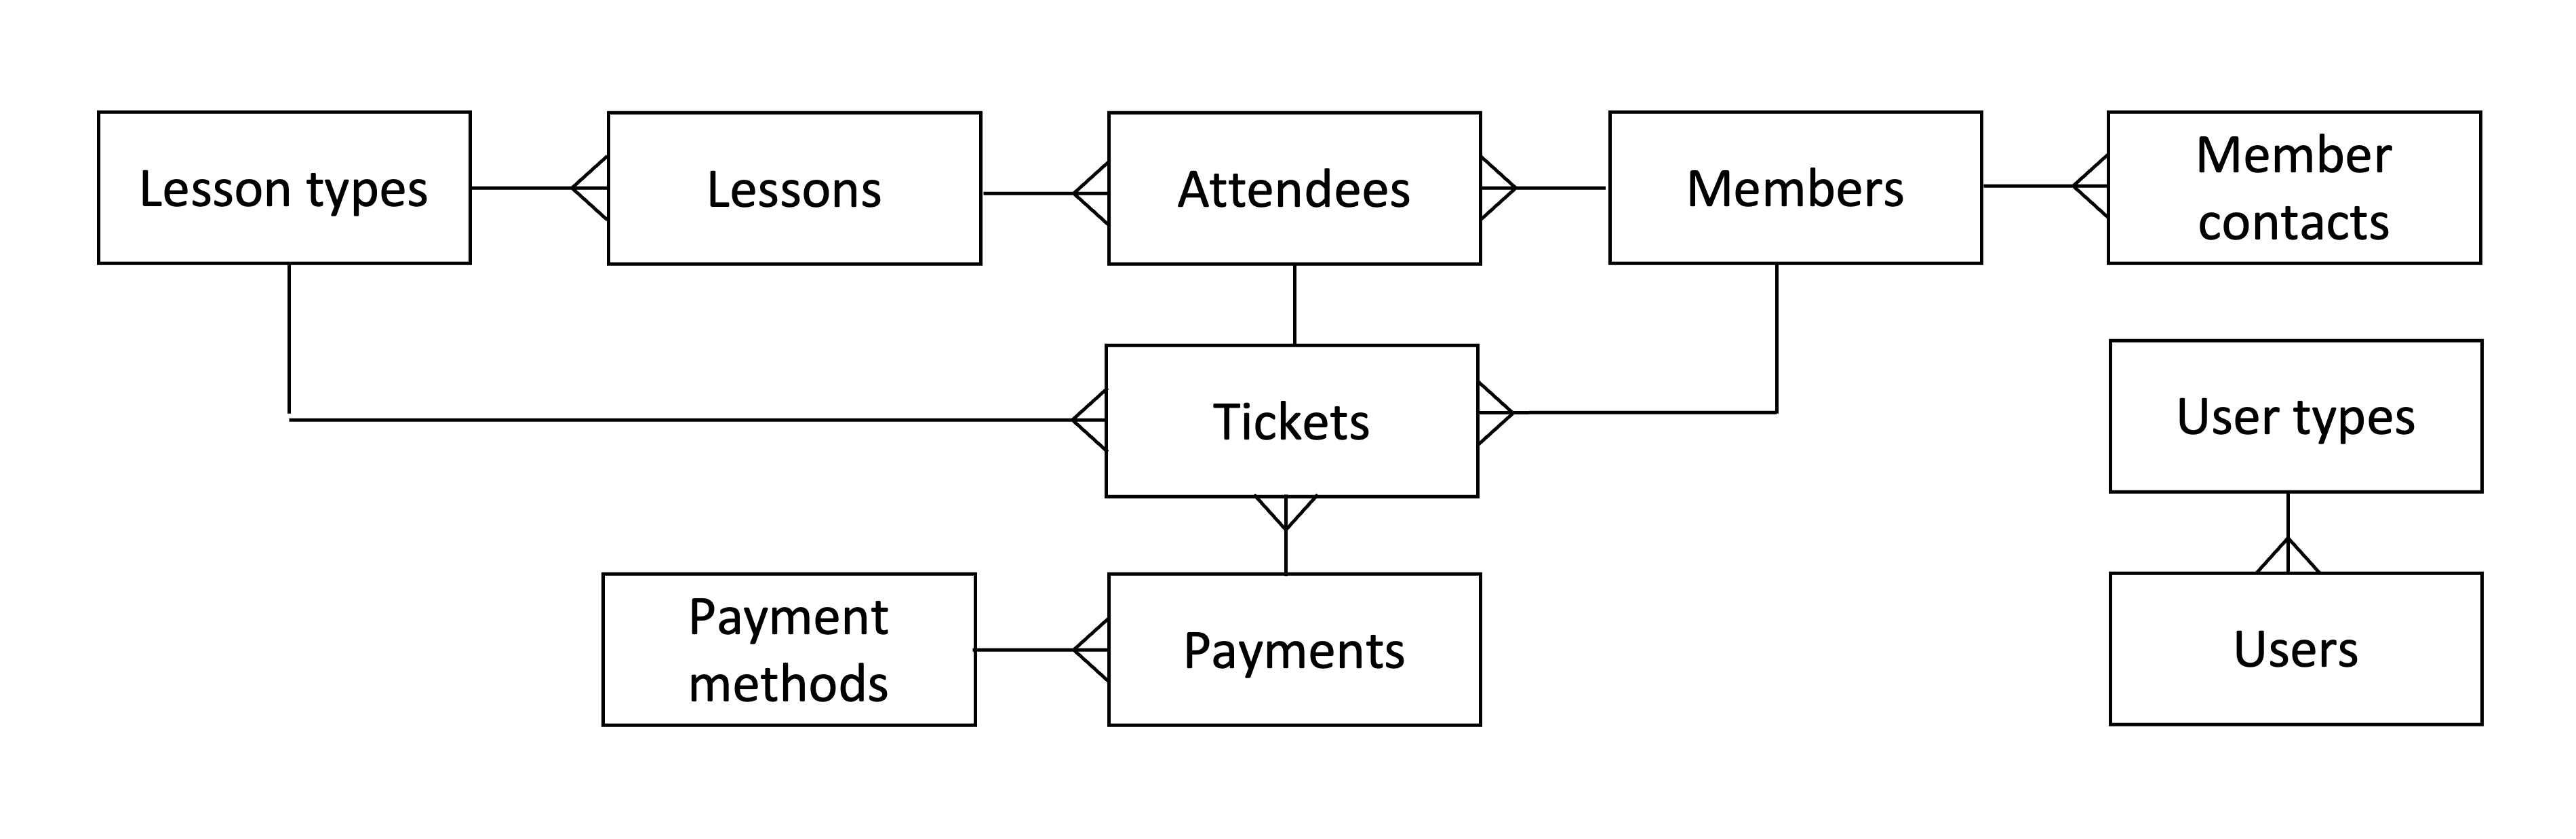
\includegraphics[width=\linewidth]{erd.png}}
    \caption{Entity relationship diagram showing the planned database table structure}
    \label{fig:erd}
\end{figure}

PostgreSQL was chosen as the relational database for this project. It is licensed under the Postgresql license, permitting use without cost or requiring written consent. Alternatives were considered, including MySQL and non-relational databases such as MongoDB; however, Postgres' performance with small and large datasets and supporting tables with relationships proved the best option for this project \parencite{arctype_performance_2021}.

Postgres also provides internal functionality for data interaction through functions called triggers. These can be activated on the change of a record and perform additional queries, including the addition, modification and deletion of records. The original intention was to use these triggers on views to prevent direct access to tables and employ the Command Query Responsibility Segregation (CQRS) pattern for payments and purchases. This design pattern segregates reads from writes, allowing greater flexibility, performance, and scalability. However, utilising this would clash with the SOLID design principle outlined at the beginning of this section, as the database would no longer only handle data storage but also perform calculations. For this reason, CQRS and event sourcing were dropped from the implementation in favour of direct table access.


%----------------------------------------------------------------------------------------
%	4. API design
%----------------------------------------------------------------------------------------

\section{API design}
The logical layer is responsible for the interaction and processing between the presentation layer's requests and the data layer's storage and retrieval in the database.

The user stories provide a flow which starts with a user interaction within the interface, triggering operations to achieve its task. Breaking down the processes within each user story revealed the operations the API would need to support to achieve each desired outcome.

Before development, the online tool OpenAPI within its online editor Swagger was used to create documentation to follow during development. It was later used to test each endpoint provided the correct response based on outlined behaviour of the documentation.

\begin{figure}[ht!]
    \centerline{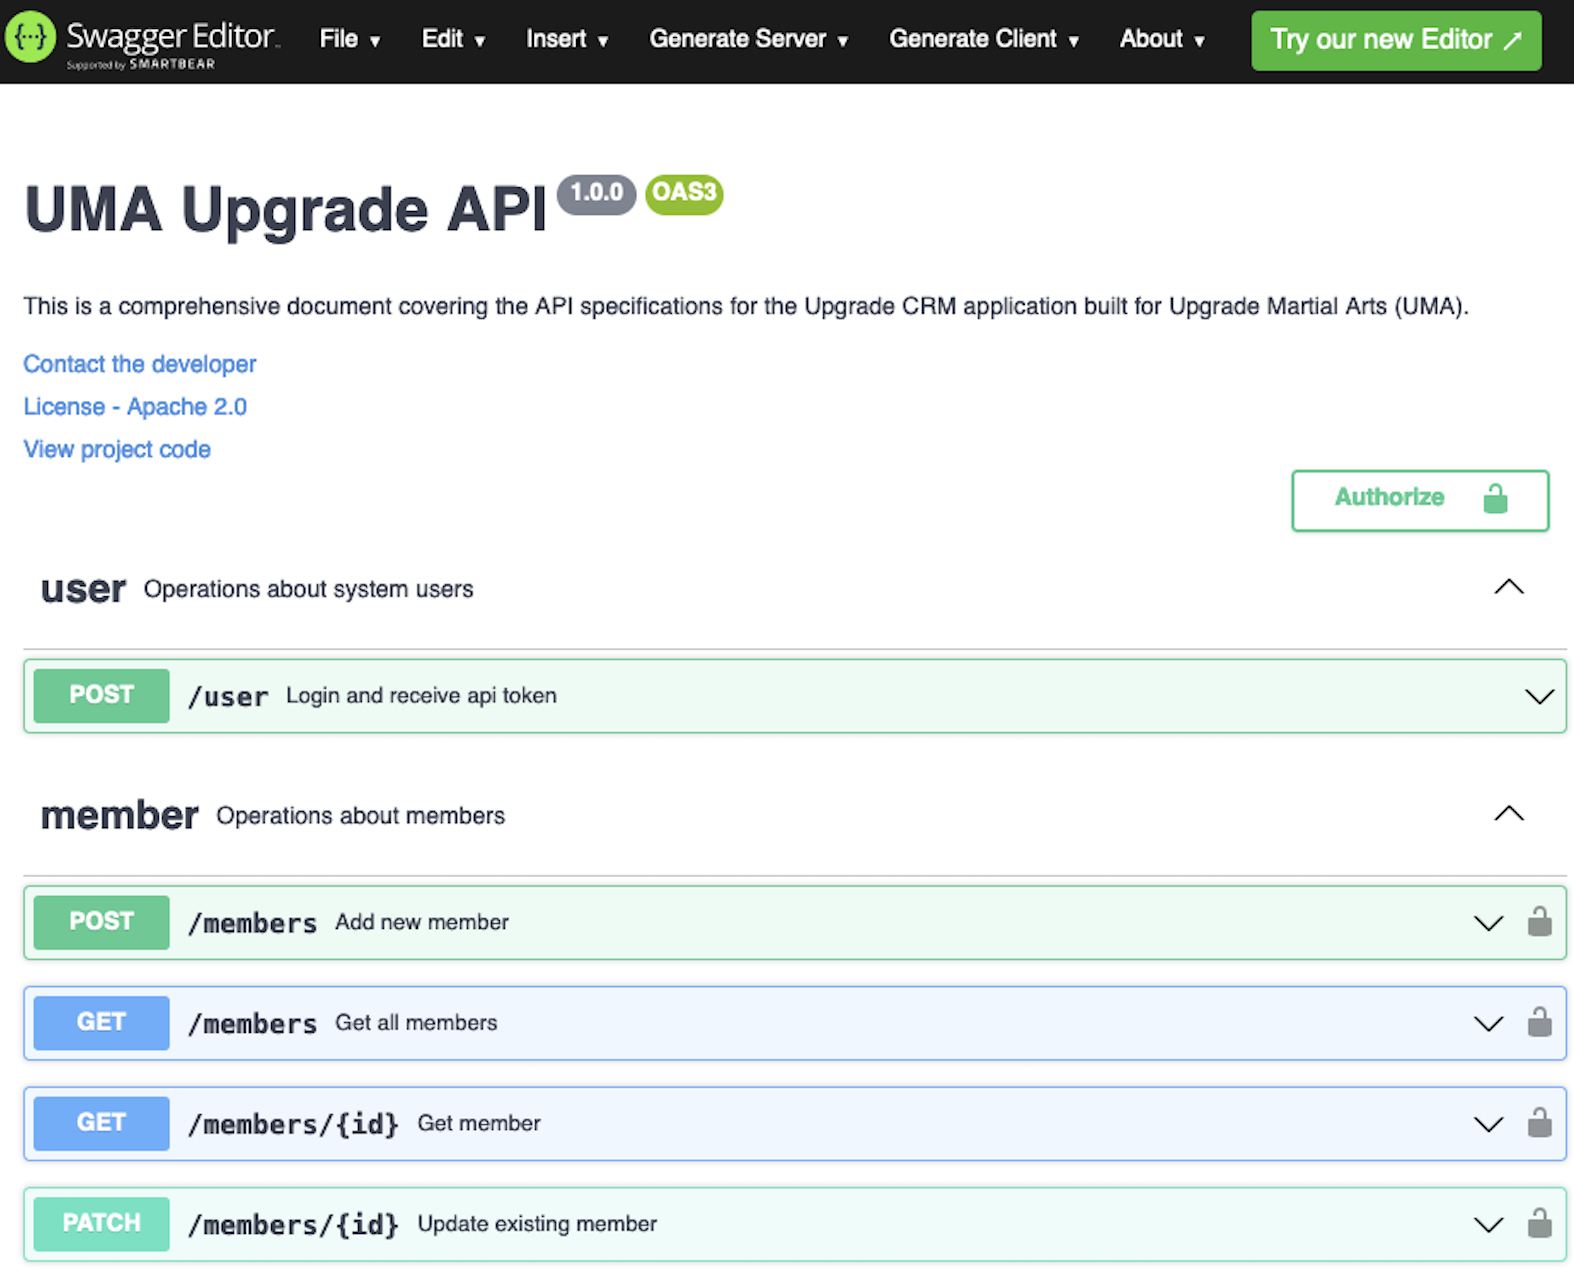
\includegraphics[width=\linewidth]{swagger.png}}
    \caption{Swagger editor showing API routes available}
    \label{fig:swagger}
\end{figure}

The MVC pattern was used in the design of the API architecture. Much like the 3-tier architecture used at the system level, the MVC design pattern also uses three layers: the model, the view and the controller.

In the context of an API, the model represents the retrieval and storage of the state within the database. These interactions could use single SQL queries to perform CRUD operations: create, read, update and delete.

The view is responsible for interaction with the logic layer and is represented as endpoints in which other software could make requests and receive responses.

The controller ties together the API endpoint and database interaction, allowing more complex operations to occur. This includes handling input validation, verifying access permissions and providing the correct error codes and responses, which were utilised heavily in each endpoint.

\begin{figure}[ht!]
    \centerline{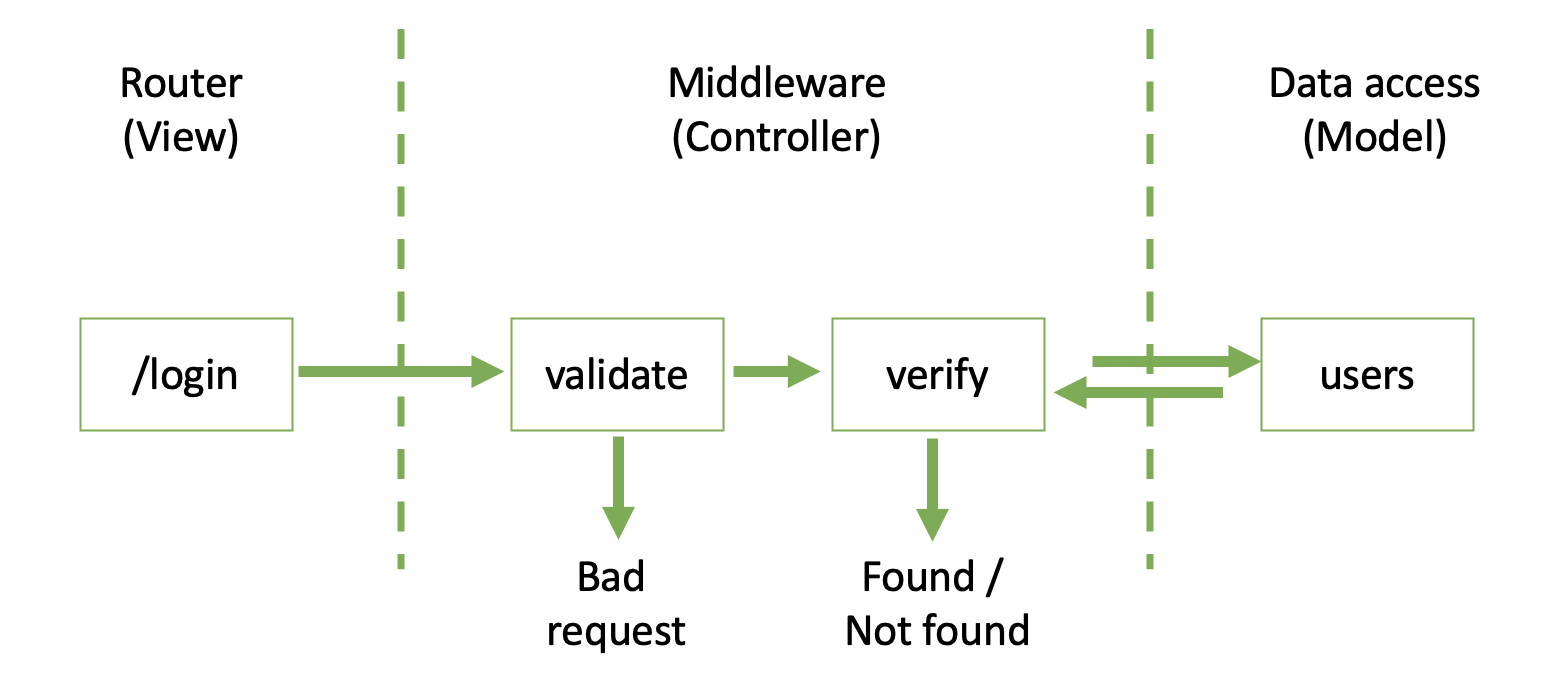
\includegraphics[width=\linewidth]{api-architecture.png}}
    \caption{API design architecture example using login route}
    \label{fig:apiarc}
\end{figure}

A flat endpoint style was implemented to simplify the interaction between the UI and API, making for an uncomplicated URL hierarchy and standardising future additions. This was further combined with standard JSON object layouts that could be easily handled and parsed at both ends.

NodeJS was selected with two main packages to interface with the presentation and data layers. The express package provided the ability to handle incoming requests and responses in a structured way. In addition, its routers provided a tidy method of segregating the launcher from each endpoint's functionality as the view. The PG package provided an interface for SQL queries on a database. These exist within service files and represent the model section of this design.

%----------------------------------------------------------------------------------------
%	5. User interface design
%----------------------------------------------------------------------------------------

\section{User interface design}

The presentation layer facilitates user interaction through inputs and visual displays representing the data. The requirements outlined the need for access across many devices. With the extreme size differences, designs for mobile and desktop views were created.

Shared components such as navigation bars, card views for summary data and common form elements, including buttons, text boxes and drop-down menus, were carefully designed. Next, the logo and colour schemes were added to these elements, where a general theme emerged and a style was established. These components were tied together into full-page designs as wireframes. These were designed to fit the user story interactions detailed in the requirements.

React selected with its component design principle. Reusable components will make a comprehensive application easier to manage. The same language as the API makes hand-off to another developer far more manageable than if the system used two different languages.

\subsection{User experience}
Great care was taken with considerations for the user experience (UX). Good UX creates a positive experience for the users of the system \parencite{yablonski_home_nodate} and makes for easier and as a result faster operation of the system.

\subsection{Wireframes}

\begin{figure}[ht!]
    \centerline{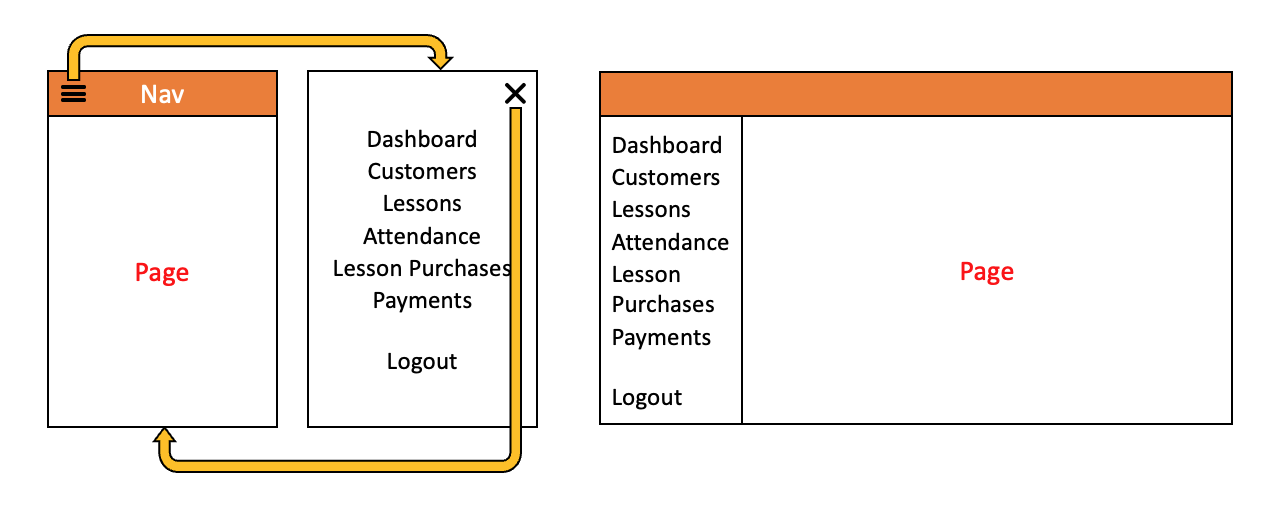
\includegraphics[width=\linewidth]{nav-wireframe.png}}
    \caption{Navigation wireframe design for mobile (left) and desktop (right)}
    \label{fig:navwireframe}
\end{figure}

\begin{figure}[ht!]
    \centerline{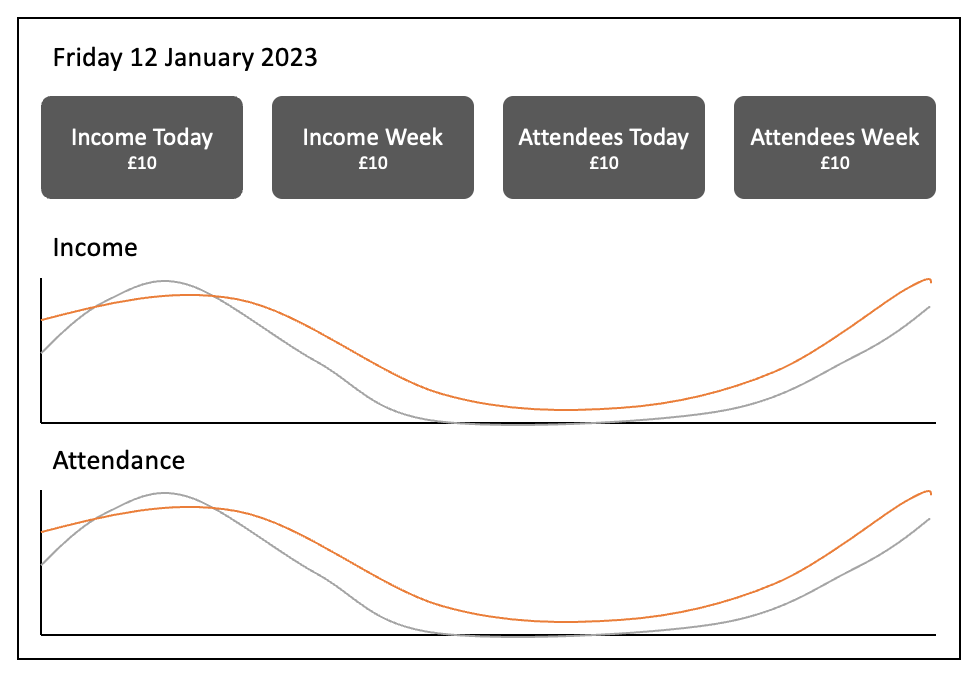
\includegraphics[width=\linewidth]{dashboard-wireframe.png}}
    \caption{Dashboard wireframe design}
    \label{fig:dashwire}
\end{figure}

\begin{figure}[ht!]
    \centerline{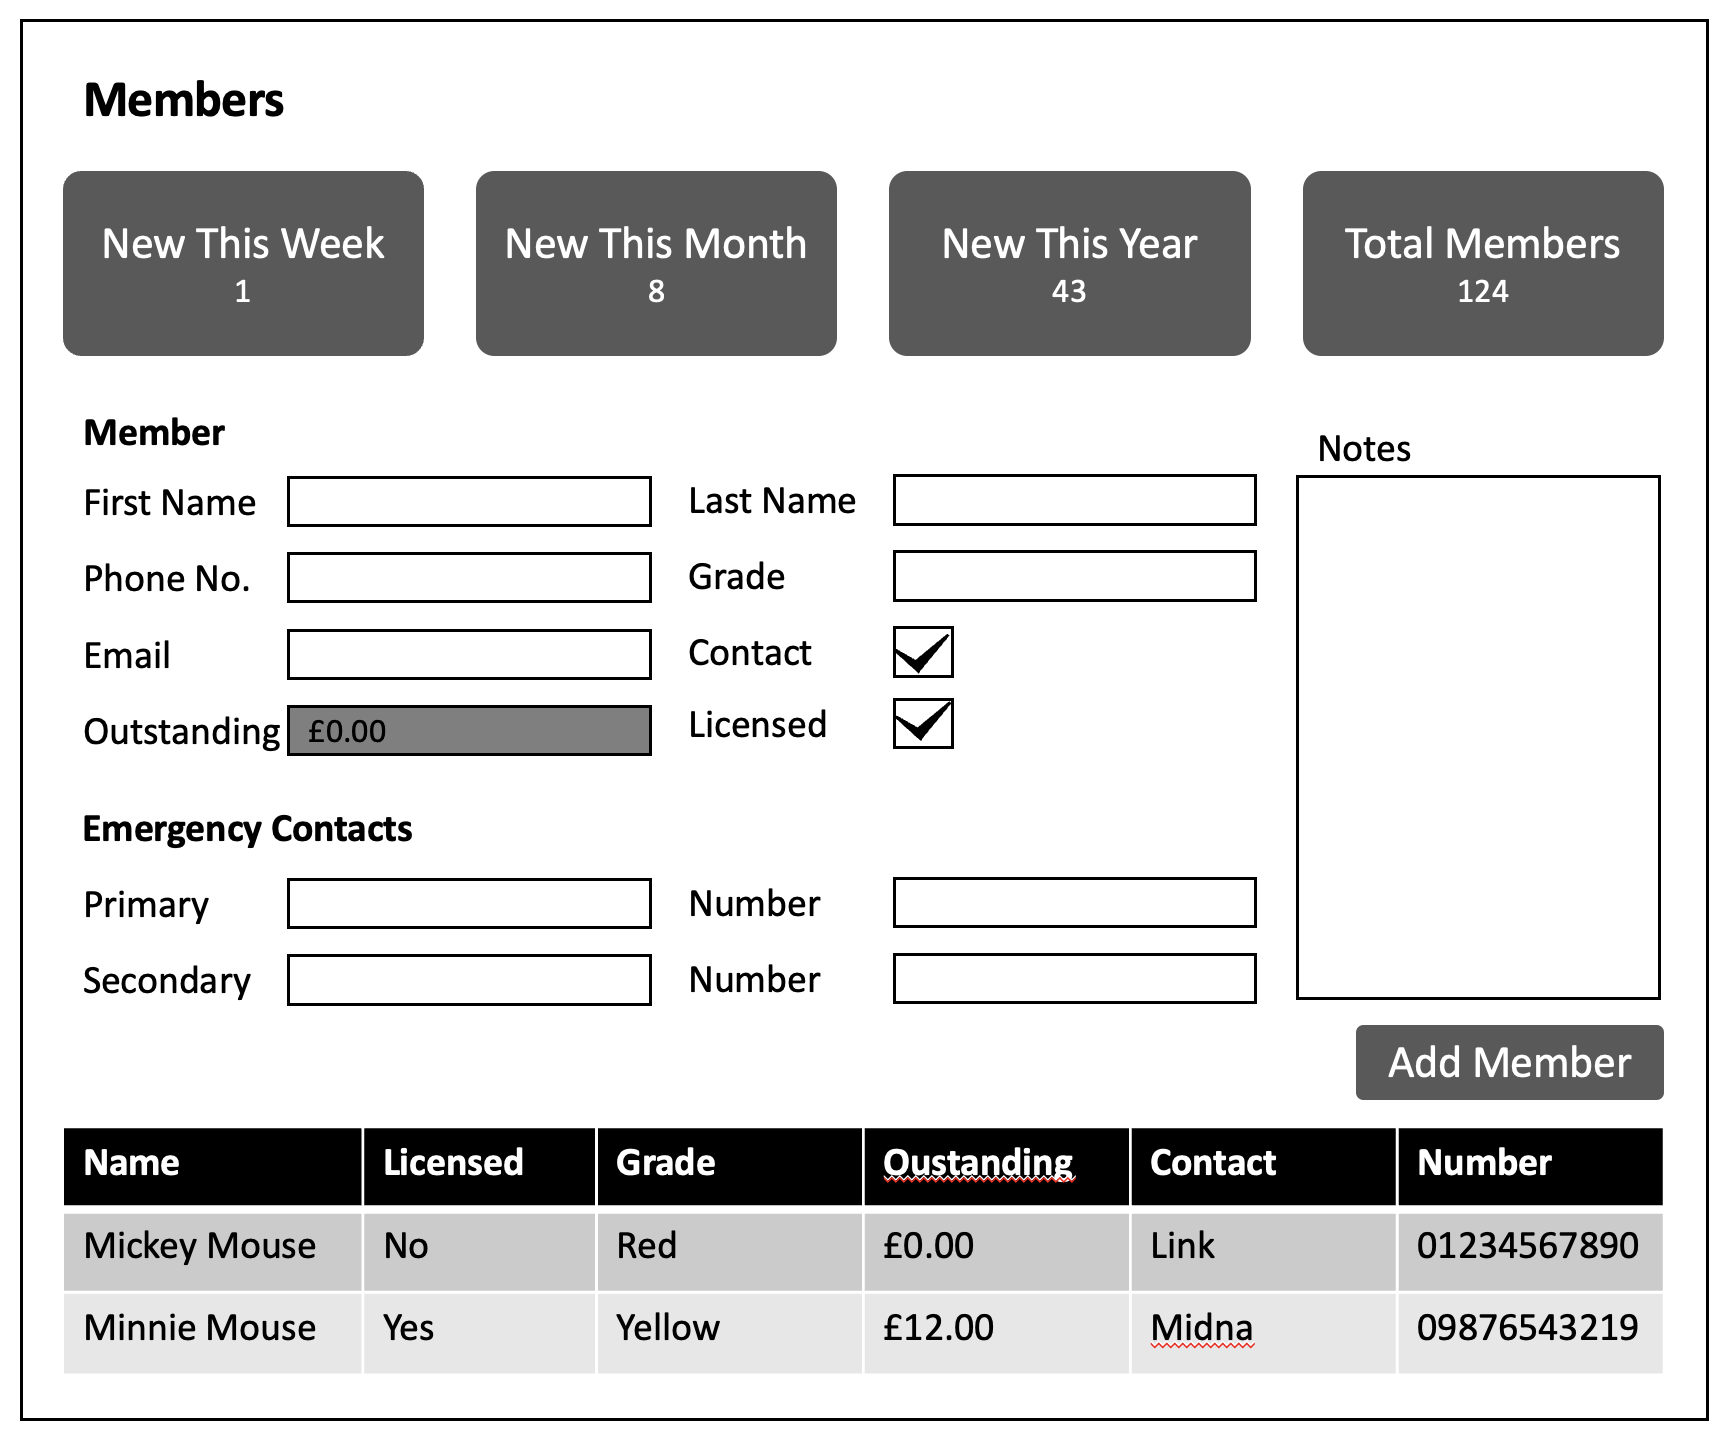
\includegraphics[width=\linewidth]{wireframe-members.png}}
    \caption{Members wireframe design}
    \label{fig:wiremembers}
\end{figure}

\begin{figure}[ht!]
    \centerline{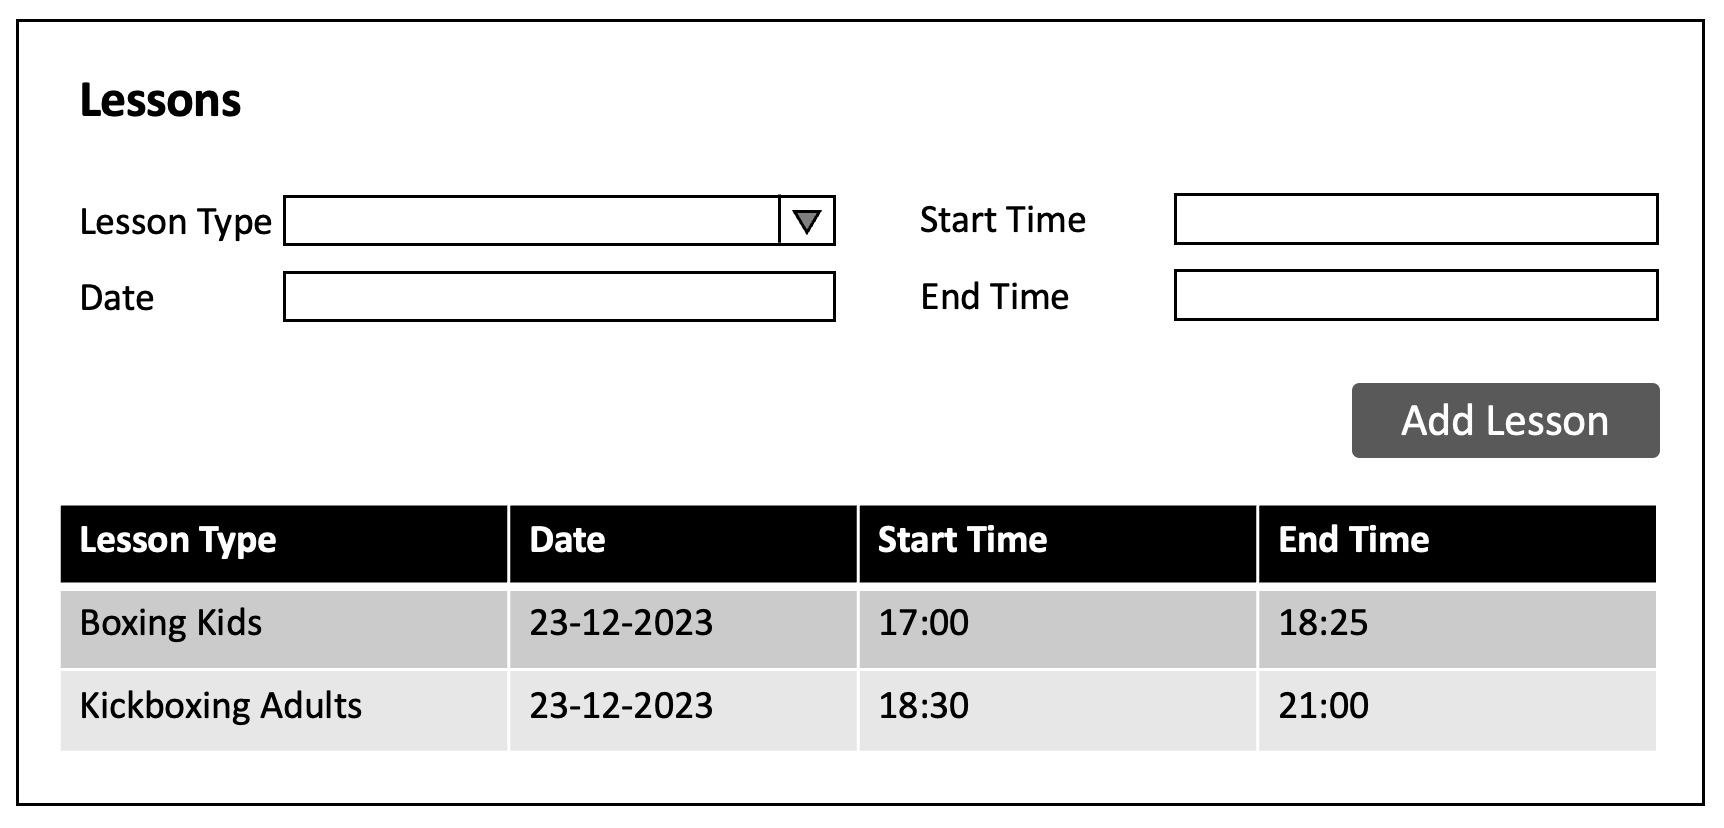
\includegraphics[width=\linewidth]{wireframe-lessons.png}}
    \caption{Lessons wireframe design}
    \label{fig:wirelessons}
\end{figure}

\begin{figure}[ht!]
    \centerline{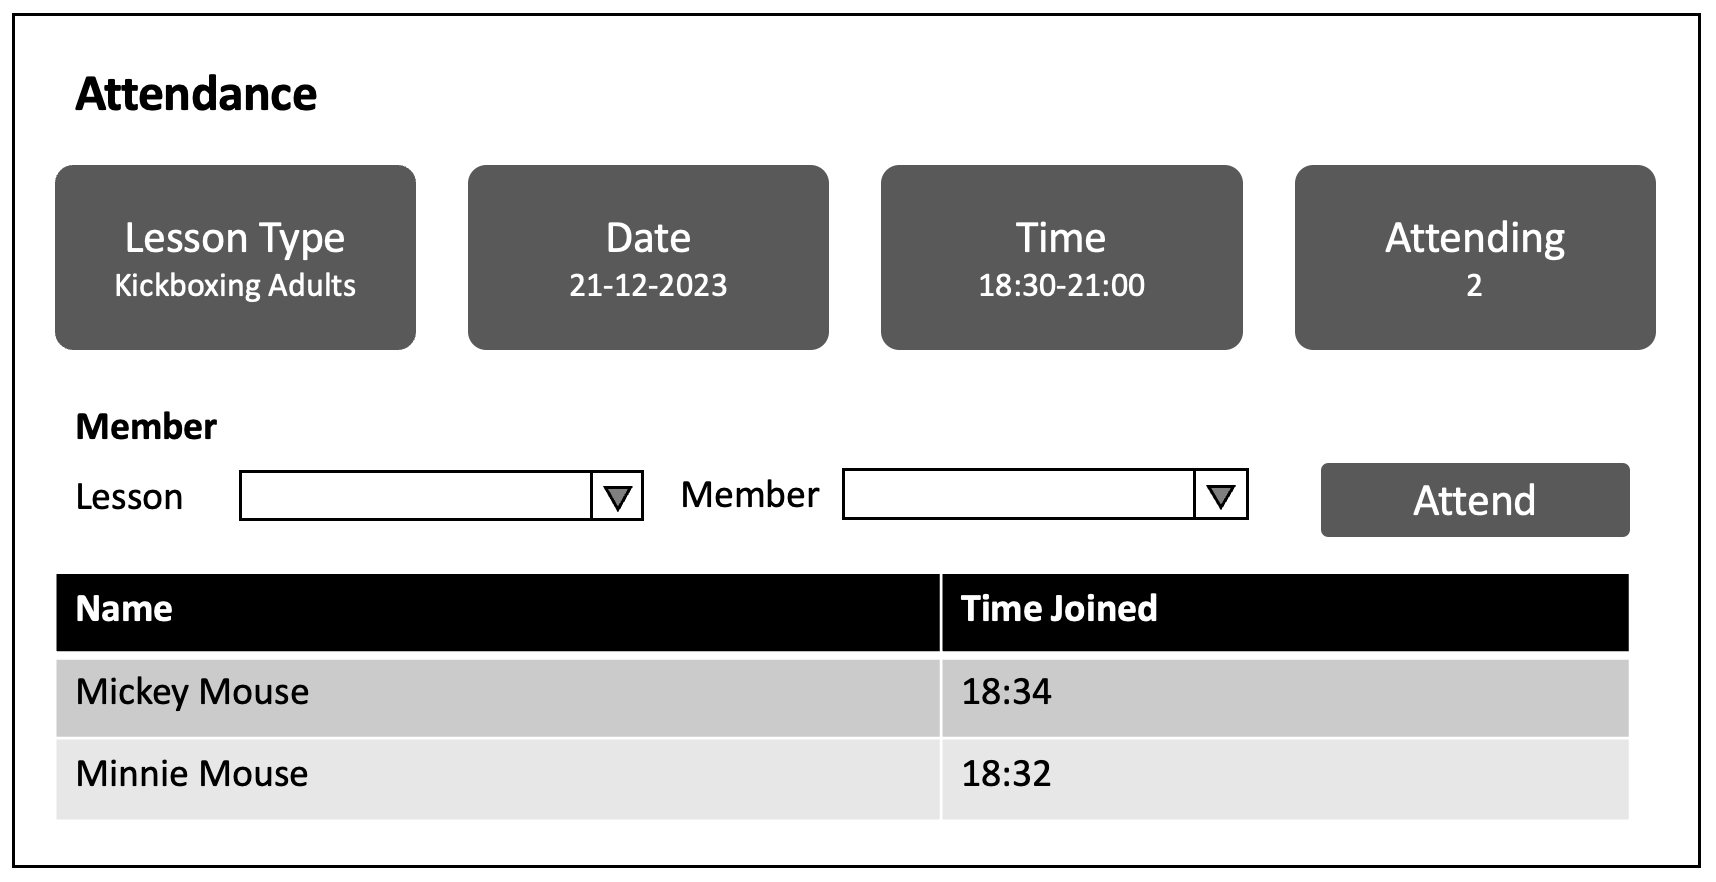
\includegraphics[width=\linewidth]{wireframe-attendances.png}}
    \caption{Attendances wireframe design}
    \label{fig:wireattendance}
\end{figure}

\begin{figure}[ht!]
    \centerline{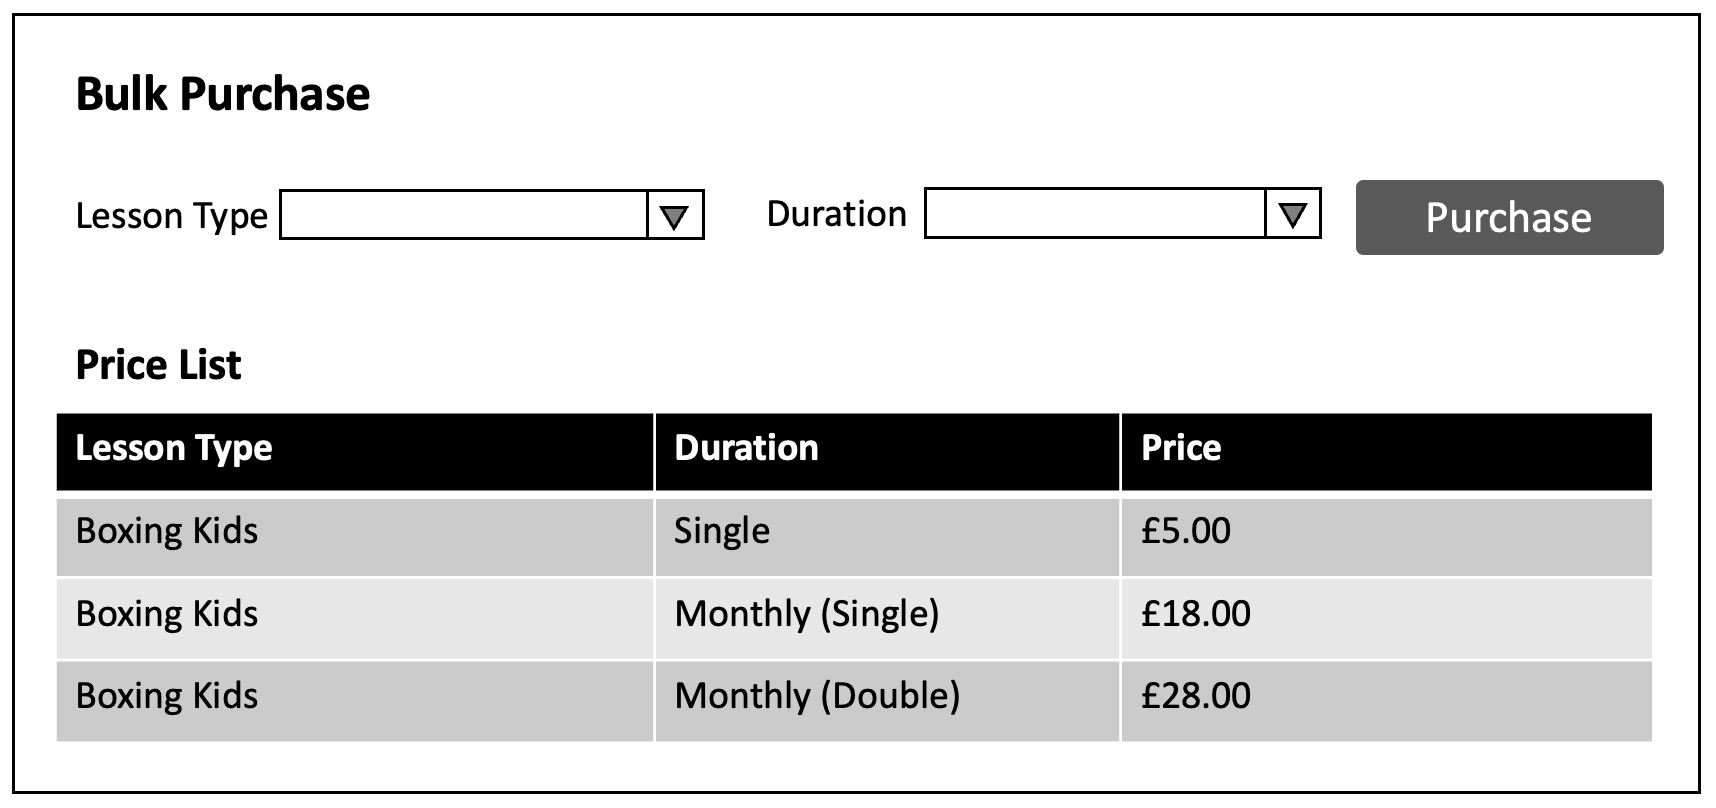
\includegraphics[width=\linewidth]{wireframe-bulk-purchase.png}}
    \caption{Purchases wireframe design}
    \label{fig:wirepurchase}
\end{figure}

\begin{figure}[ht!]
    \centerline{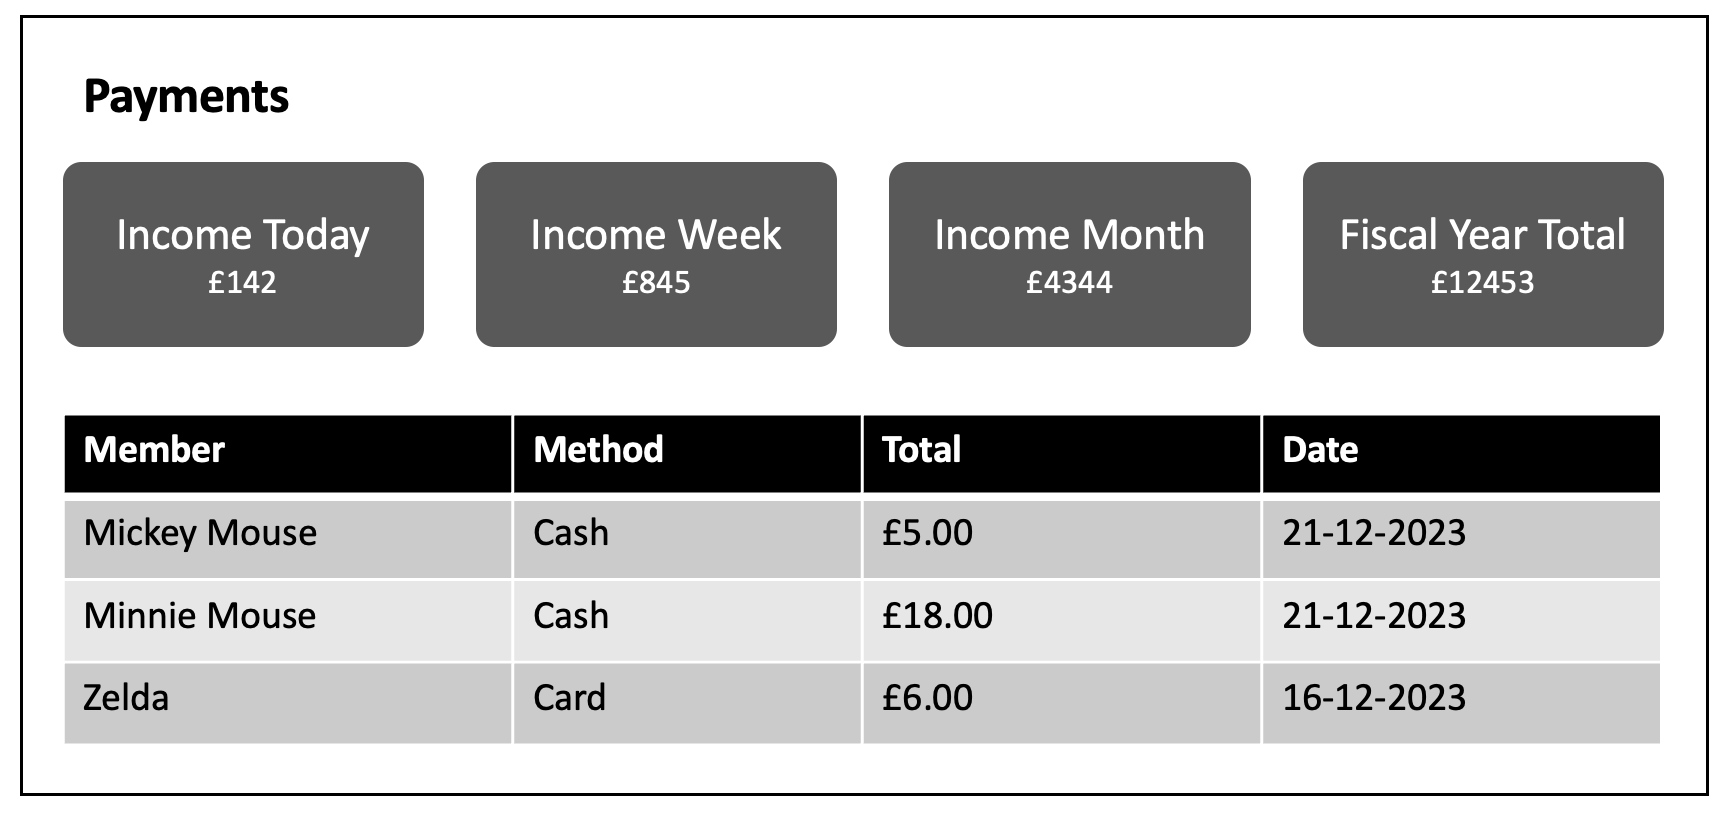
\includegraphics[width=\linewidth]{wireframe-payment.png}}
    \caption{Payments wireframe design}
    \label{fig:wirepayments}
\end{figure}

%----------------------------------------------------------------------------------------
%	6. System deployment
%----------------------------------------------------------------------------------------

% \section{System deployment}

% Todo
 % Product Description
%----------------------------------------------------------------------------------------
%	Project management
%----------------------------------------------------------------------------------------
\chapter{Project management} % Main chapter title
\label{Chapter5} % For referencing the chapter elsewhere, use \ref{Chapter5}

This section covers the management of the project, including the project's lifecycle during development, the software testing involved with ensuring all operations are functional, and what methods were used to mitigate risk guaranteeing the project's success.

%----------------------------------------------------------------------------------------
%	1. Project life cycle
%----------------------------------------------------------------------------------------

\section{Project life cycle}

Development of the project utilised the agile approach consisting of two-week sprints focused on delivering features. Rather than building and implementing each layer, the system was built using vertical slices. Each requirement consisted of a slice of the project from UI to API to the database and back again. Each slice was added over time to assemble the complete system which follows the FDD approach.

The full list of completed actions for each week during the planning stage and each sprint during the development stage has been tracked in Trello (Appendix \ref{AppendixA:Trello}), and time management in the Gantt chart (Appendix \ref{AppendixA:Gantt}).


\subsection{Environment setup}
Development started with setting up the development environment, which included creating the GitHub repository and linking it to the development system.

The Trello board was then created to list all system requirements and allow for tracking work completed each sprint.


\subsection{MVP - Login and Members}
A minimum viable product (MVP) was created to start the development of the system stack. The minimum the business requires to start is a member storage and view combined with a method of access control through a login system.

\begin{figure}[ht!]
    \centerline{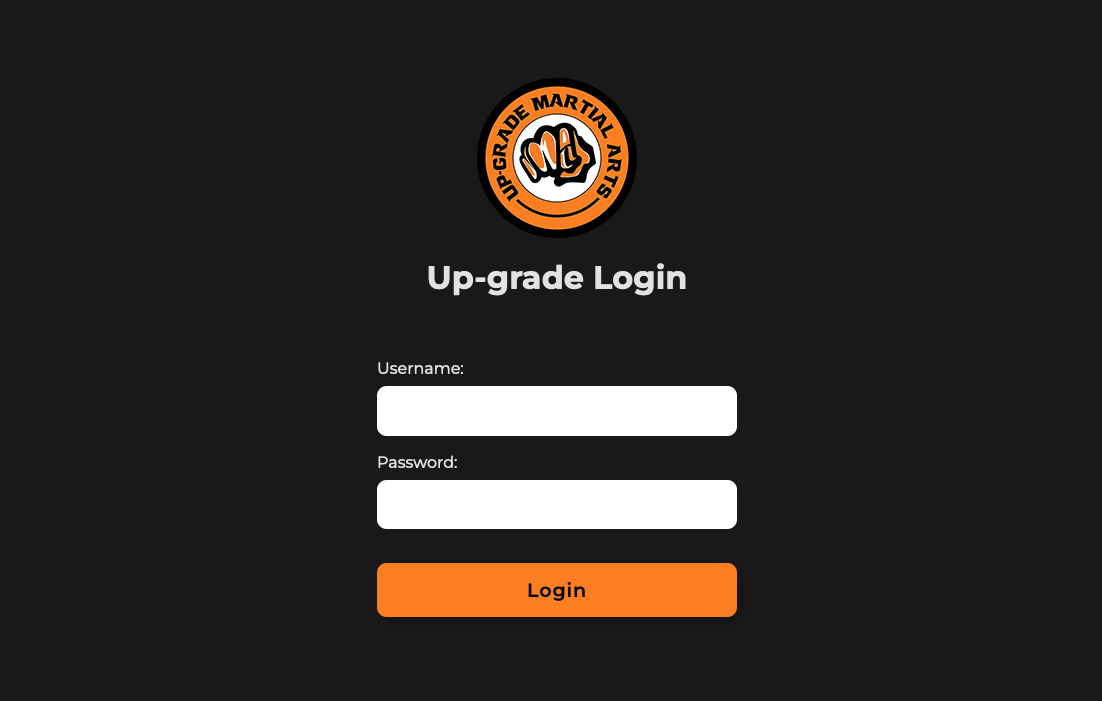
\includegraphics[width=.9\linewidth]{login.png}}
    \caption{Implemented login screen including logo and form}
    \label{fig:login}
\end{figure}


The login system \parencite{adams_basic_2018} \parencite{macharia_session_2021} is vital in securing the system from unauthorised access to stored personal and business data. Access control became the first system implemented for this reason.

The database was initially created with the 'users' table to store the staff usernames and passwords. The creation of this table was added to the schema file, and default login details were provided in the seed file.

The API was then initialised to support a POST endpoint to receive login data and provide a response if a matching record was found in the database. The 'express' package provided the interface for receiving HTTP requests, and the 'pg' package for interfacing with the database. The database connection details were added through environment variables since they change and connection made using a connection component.

\begin{figure}[ht!]
    \centerline{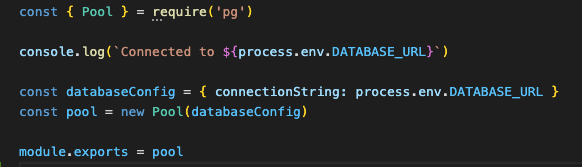
\includegraphics[width=.9\linewidth]{dbconn.png}}
    \caption{Database connection component using environment variables to connect}
    \label{fig:dbconnect}
\end{figure}

Research into best practices \parencite{page_how_2023} revealed the need to store passwords as encrypted strings \parencite{gauravaram_security_2012} rather than plain text. This encryption is to prevent system administrators from gaining customers' login data, which they could exploit, and also stop malicious actors such as hackers from using the details should the database become compromised or leaked.

\begin{figure}[ht!]
    \centerline{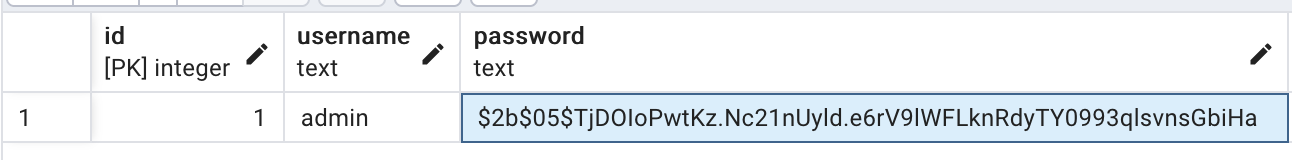
\includegraphics[width=.9\linewidth]{encrypted-password.png}}
    \caption{Salted and hash encrypted password}
    \label{fig:password}
\end{figure}

The 'bcrypt' package was added to provide functionality for salting and hashing the received passwords. Now, passwords stored in the database are encrypted (Figure~\ref{fig:password}). The received password is put through the same method to salt and hash, then compared to check if login details match.

If successful, the API returns a JSON Web Token (JWT) containing necessary user data, such as their ID, alongside an expiration date and time when the token is no longer usable. This token can only be opened by the server making the data stored inside secure and preventing impersonation from maliciously crafted tokens.

This token can now be appended to data requests where the server can open and verify credentials allowing a request to succeed. This verification method within the API was created as middleware which can be attached to any endpoint, enforcing the requirement of a valid bearer token to access the data.

A new form was created in the UI, which allows entering a username and password in combination with a button to submit the login request. This request is sent to the API and handles the response received. If the token is returned with a 200 response code, the token is stored, and the app component is rendered through React's hooks. A corresponding error message is shown to the user if an error response is received.

With the app secured with access control, data can now be stored. A new table was created to hold member data based on the normalised form created during development. This table was added to the schema file for generation upon new database creation.

\begin{figure}[ht!]
    \centerline{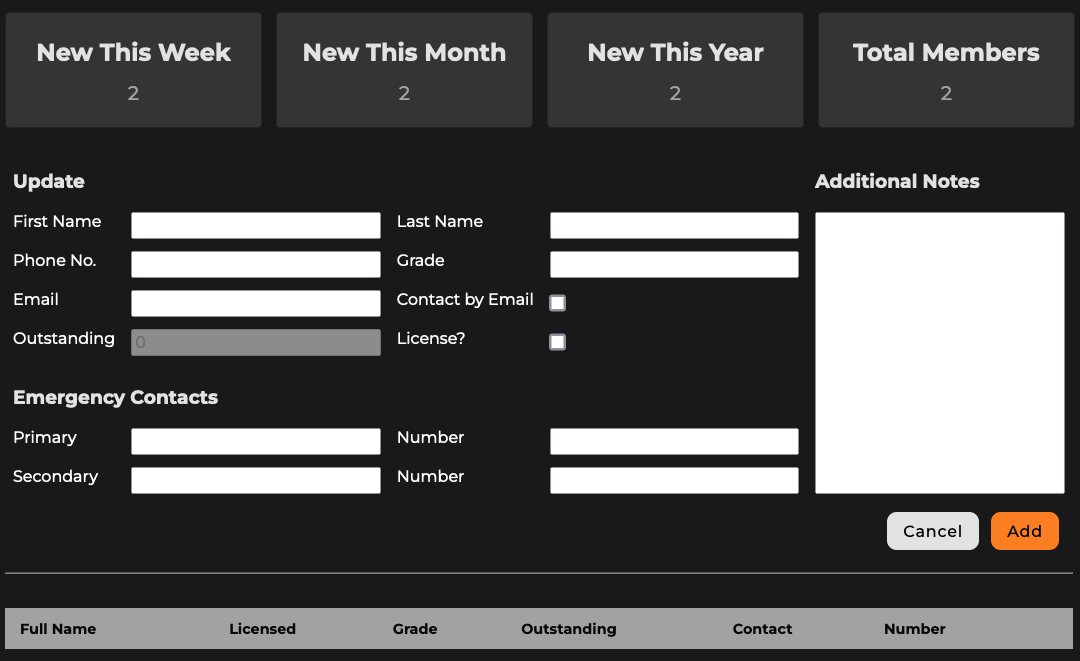
\includegraphics[width=.9\linewidth]{members-page.png}}
    \caption{Implemented members page}
    \label{fig:members-page}
\end{figure}

Three endpoints were added to the API to support viewing all members, adding a new member and editing an existing member referenced by ID. In addition, validation of inputted data and verification of a bearer token was added as middleware, preventing error cases such as missing required fields and expired or missing tokens.

Finally, the UI must support viewing all member data, the input of new members who are registering and updating existing members already recorded in the system.

A table view was first created to display all members. A fetch request to the API returns an array of members, which are mapped for easy searching based on their ID. This map is then iterated over to create the rows in the table.

Afterwards, a form was created to input new member data, which could then be submitted to the API for storage. The form had the required fields match those found in the database and would be verified within the API middleware. This consistency would prevent accidental errors in input by preventing submission without the requirements met.

This form could be reused to update existing members if provided with an ID. The table was altered to support an 'onClick()' event where a function could be performed when the selected row was clicked. This function sets an active id variable rendering the form with the data filled into the fields for altering. The active id also changes the behaviour of the form submission by changing the request from a POST to a PATCH utilising the update route instead of the add route (Figure~\ref{fig:members-patch-post}).

\begin{figure}[ht!]
    \centerline{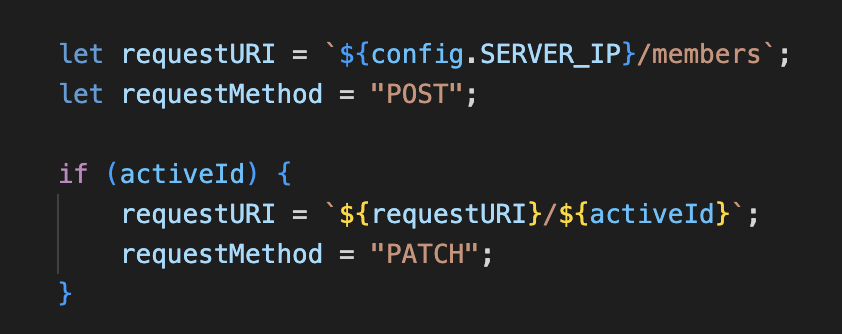
\includegraphics[width=.6\linewidth]{post-or-patch.png}}
    \caption{If check for adding or updating a member's record}
    \label{fig:members-patch-post}
\end{figure}


\subsection{Sprint 1 - Lessons}

This first sprint focused on storing lessons and the required lesson types. In order for lessons to be stored, their lesson types must be stored first which they can then reference. The lesson types consists of "Boxing (Kids)", "Boxing (Adults)", "Kickboxing (Kids)", "Kickboxing (Adults)" and "Yoga".

A table was created to hold these values along with a referencable ID (Figure~\ref{fig:lesson-types-schema-sql}). The lesson types are added as non-editable, static values to the database (Figure~\ref{fig:lesson-types-seed-sql}). A route was added to get all rows. Since the values are static, there is no need for POST or PATCH to handle adding or updating respectively.

\begin{figure}[ht!]
    \centerline{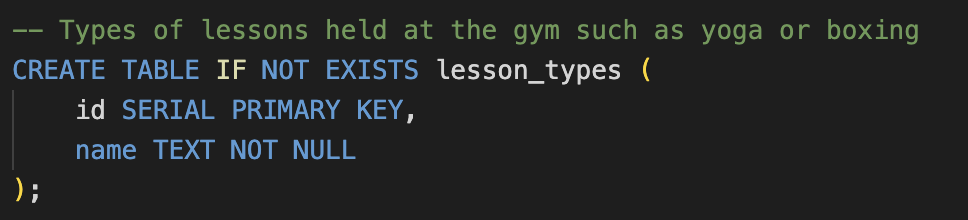
\includegraphics[width=.9\linewidth]{lesson-types-sql.png}}
    \caption{Lesson types sql schema}
    \label{fig:lesson-types-schema-sql}
\end{figure}

\begin{figure}[ht!]
    \centerline{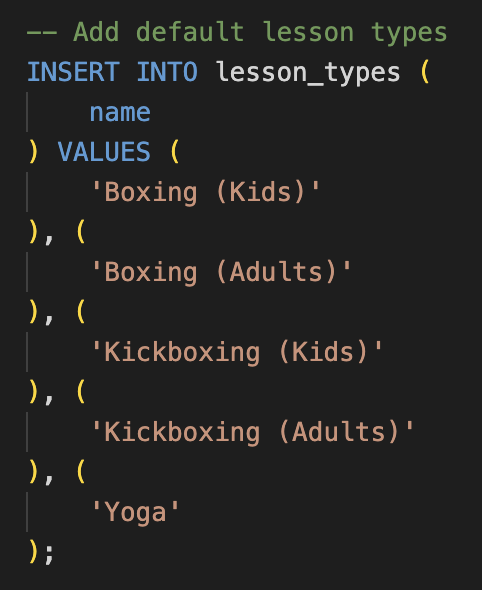
\includegraphics[width=.4\linewidth]{lesson-types-seed-sql.png}}
    \caption{Lesson types sql seed}
    \label{fig:lesson-types-seed-sql}
\end{figure}

The interface also matches this static state of the table by not providing a method to edit the data. The records are instead stored within the user interface as a map which is retrieved upon login. This way we prevent future requests and unnecessary network requests for the data by keeping a single local copy.

Lessons can be added now that the types have been defined and are retrievable. The lesson were created by first creating the database schema. The table contains a foreign key linked to the lesson types table. Now the lessons can contain a referenced type. This is useful for searching functionality and in the future for lesson attendance based on lesson type.

\begin{figure}[ht!]
    \centerline{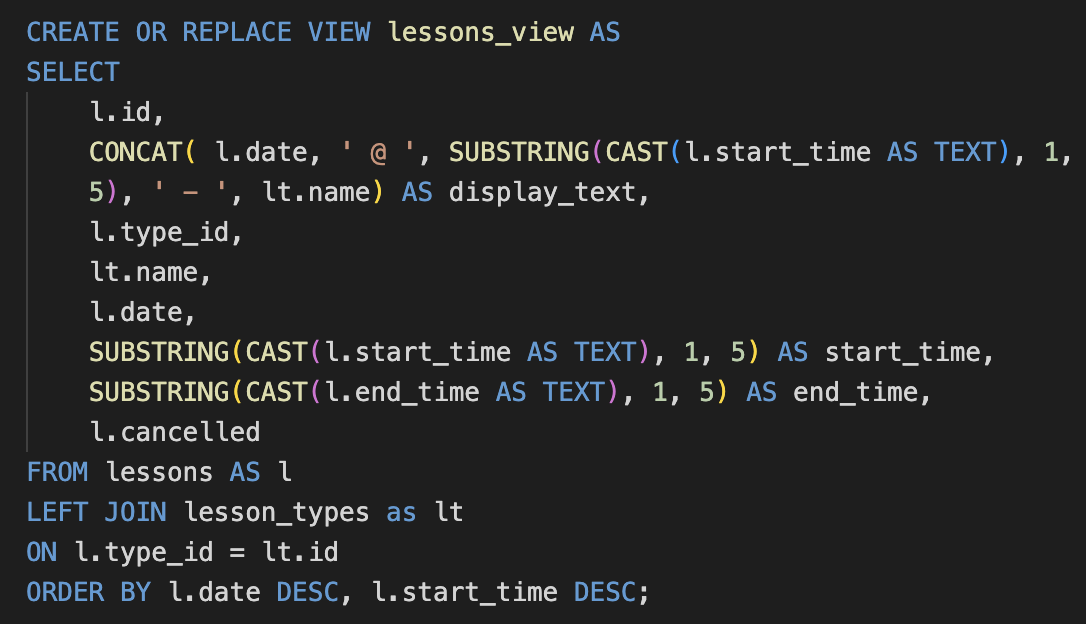
\includegraphics[width=.8\linewidth]{lessons-view-sql.png}}
    \caption{Lesson view sql schema}
    \label{fig:lesson-view-schema-sql}
\end{figure}

A view was also created within the database to get the data including labels from the linked table as text (Figure~\ref{fig:lesson-view-schema-sql}). This prevents the need to manually search each table and instead get all necessary values in a single query. This also results in lower network utilisation through less queries.

Next the routes were added to the API for requesting all lessons, adding new lessons and updating existing lessons. This followed the same structure as the customers table. The get request references the view providing this useful reduced search information.

Finally adding new page to the UI to interact with the API endpoints created for input, view and updates. New form elements had to be utilised, including date and time selectors.

\begin{figure}[ht!]
    \centerline{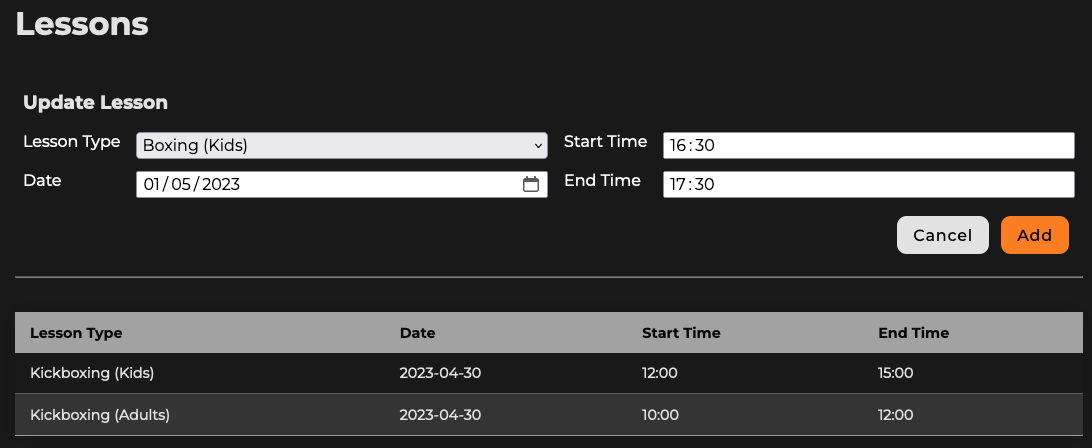
\includegraphics[width=\linewidth]{lessons-page.png}}
    \caption{Implemented lessons page with form and table}
    \label{fig:lessons-page}
\end{figure}

A more complex element was the drop-down menu. Lessons have required lesson types. The selected value is that of the ID rather than the text contained within. This was complex and required creating a new customisable component which can now take any map of values and create a drop-down. When the value is changed, a callback function can update a stored variable and trigger other changes too.

\begin{figure}[ht!]
    \centerline{
\includegraphics[width=\linewidth]{custom-drop-down.png}}
    \caption{Custom drop-down menu using data fetched from the API}
    \label{fig:drop-down}
\end{figure}

This sprint's work lays the foundation for pricing, purchasing and eventually attendance of members to these lessons.


\subsection{Sprint 2 - Lesson Pricing}
The pricing structure requires different prices for different lesson types and durations. We have the lesson types defined from the last sprint so the lesson purchase types to differentiate the prices is now required.

The table was created to store the purchase types: day single, weekly single, weekly double, weekly triple, and weekly unlimited. This was added to the schema file and the database updated to include the new table.

Using these two tables, the table lesson pricing was created and prices added to the seed file. This table combines the lesson types and purchase types to allow the storage of the comprehensive price list.

\begin{figure}[ht!]
    \centerline{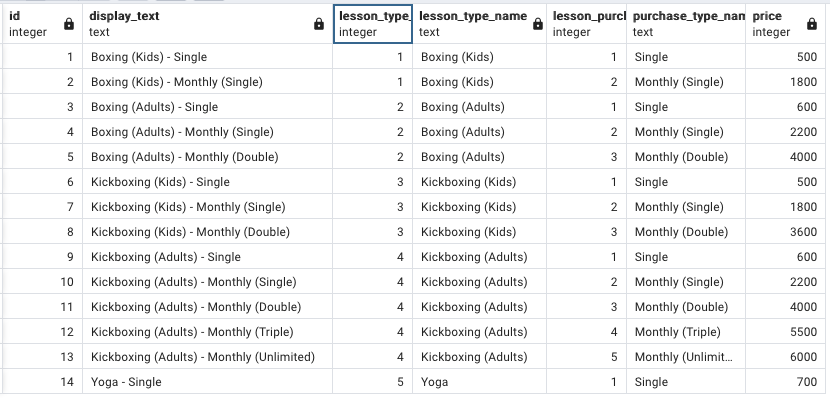
\includegraphics[width=\linewidth]{lesson-pricing-tables.png}}
    \caption{Database view of lesson pricing table with left joined lesson type and purchase type}
    \label{fig:lesson-price-view}
\end{figure}

Routes were added to the API allowing requests for the purchase types and the prices. The prices are retrieved from a view which includes the lesson and purchase types. This aids in the display of these prices in drop-down selection boxes.

During planning these were listed as static values, however prices may require updating in the future requiring a patch to the database to do this. This was a large oversight during the design stage. Although there is no interface designed, a route for updating the prices has been included for easier developer maintenance.

\begin{figure}[ht!]
    \centerline{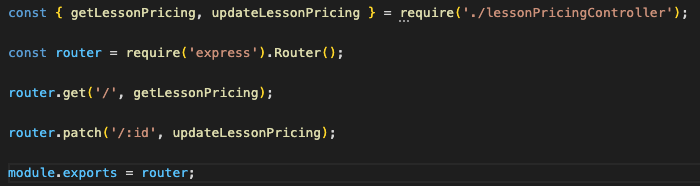
\includegraphics[width=\linewidth]{pricing-patch.png}}
    \caption{Update route for lesson pricing}
    \label{fig:pricing-patch-router}
\end{figure}

The purchase types and prices were added to the interface for storage on login. With these values now stored, lesson purchasing and payments can be focused on next. This will lead gracefully onto tracking the attendance in a later sprint.


\subsection{Sprint 3 - Lesson Purchasing}
With lessons and pricing now functional, a record of payment and methods are required to start making lesson purchases.

Payment methods are a simple static table which holds the different payment methods the business supports. They have explicitly specified they only accept cash and card payments only. The data could be stored statically within the application and text saved however for indexing and data consistency, a new table for payment methods was created.

Payments were then created to hold a record of all income made from lessons. The payments consist of the member who made the payment, method of payment, the total amount paid and when the payment was made.

If the prices can now update in the future, we cannot rely on the stored prices to track history purchases and payments. For this reason, the tables include their own prices which reflect the calculated price at the time of purchase.

\begin{figure}[ht!]
    \centerline{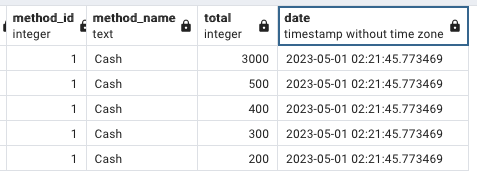
\includegraphics[width=.8\linewidth]{payments-table-snapshot.png}}
    \caption{Database payments table tracks total without links}
    \label{fig:payments-total}
\end{figure}

Lesson purchases combine the member, lesson type, duration through purchase type and the payment made to track what members have made what purchases. This increases the accuracy of the data stored which can be further used for business analytics.

Static route was added for payment methods and like all prior static data is retrieved upon login. The payments are handled internally within the API as a middleware. The lesson purchase API route includes this payment middleware by using the submitted data to determine the payment data and adds it when a lesson is purchased. This automated nature and removal from the UI simplifies the external interface removing unnecessary endpoints and making interaction far easier.

Lesson purchases screen created using the wireframe and interfaces with the API endpoint. A price list is shown on this screen which required uses the prices data the interface holds. This is useful when customers inquire about prices removing the need for print outs or searching files on the computer or phone.

% Add screenshot of price list table and purchase form

The attendance could be tracked using this, however would require a great deal of calculation upon each validation request. To increase efficiency and improve the scalability of the system, the token system will be implemented in the next sprint.


\subsection{Sprint 4 - Tokens}
Members can now purchase lessons and now must be able to use these purchases to attend lessons.

In need of an efficient system to track attendance based on week and month, a ticket system was implemented to solve this issue. Based on lesson purchase type and lesson type, a token representing a valid pass for a particular lesson during a particular period would solve the problem.

Also solved the issue of a free first lesson for new members. A token without a set lesson type could be used to be a general pass, and an expiration date of 1 year would be sufficient, which the member could claim.

First a table to track the tokens issued. The token is issued to a member with an activation start date for when the token starts being valid and an expiration date when the token is no longer usable. Finally, there is a used flag which can be set to invalidate the token however keep it in the system for metrics data.

A view was created of these tokens to only show unused tokens making further searches faster by working on a subset of the data.

\begin{figure}[ht!]
    \centerline{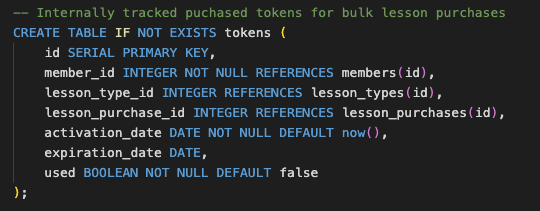
\includegraphics[width=.8\linewidth]{token-table.png}}
    \caption{Token table schema}
    \label{fig:token-table}
\end{figure}

An endpoint to request the next valid token based on the member id was created for the future attendance screen. This was done by first querying for tickets that are for the active lesson type. On the subset of results they are checked if they are not yet used, the start date is before the current date and the expiration is after the current date. If a valid token is available, the ID may be used to allow attendance to a lesson. This was tested with custom crafted tokens.

To generate tokens is more complicated than filtering. First the API requires a member, lesson type and purchase type to determine who gets the tokens, how many to generate and what date range each are for. The purchase type table was modified to include the number of tokens to generate, the duration in days each token is valid for and how many weeks of these tokens to create. The lesson purchase route was extended to include the generate tokens middleware. Now when lessons are purchased, tokens which correlate to the purchase are generated and stored for the specified member. 

\begin{figure}[ht!]
    \centerline{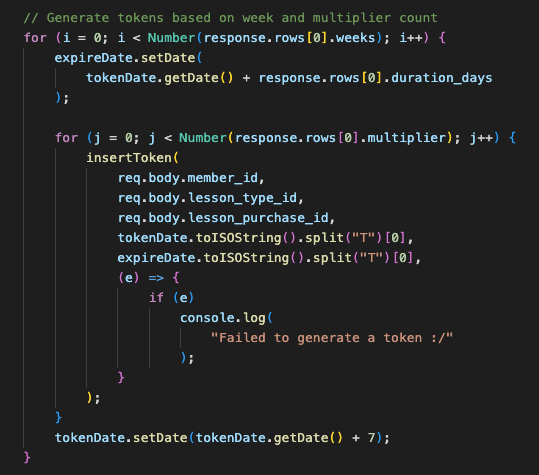
\includegraphics[width=.8\linewidth]{generate-tokens.png}}
    \caption{Code to generate tokens on lesson purchase}
    \label{fig:purchase-gen-tokens}
\end{figure}

These tokens can now be used to attend lessons which is the focus of the next sprint, sprint 5.

\subsection{Sprint 5 - Attendance}
The next step is to track member attendances to lessons. The attendance is made up of members in combination with lessons. The limiting factor which has now been addressed is the tokens allowing participation in particular lessons. The attendance date is tracked for metrics and statistics which can be displayed on the dashboard.

In the intial iteration of the attendance tracking tokens were not required and the attendance was tracked by the member and lesson type. This was later changed to require tokens to attend once attendance was implemented.

\begin{figure}[ht!]
    \centerline{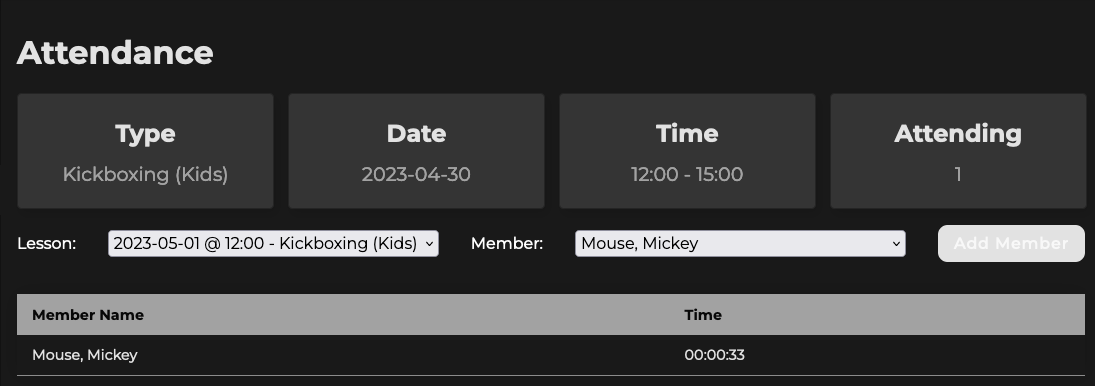
\includegraphics[width=\linewidth]{attendance-screen.png}}
    \caption{Attendance implemented screen}
    \label{fig:attendance-screen}
\end{figure}

The next hurdle lies with members wishing to pay later and within the same screen. An option for members to pay now or later was added as a component that can trigger the same purchase endpoint; the lesson purchase screen has already implemented the required behaviour making extension of this simple in thanks to the MVC architecture.

To manage pay later, attendances could be made without a token. This would prompt the API to append the price of the lesson to the outstanding amount in the member's record.


\subsection{Sprint 6 - Statistics and Metrics}
With the core functionality the receptionist will be utilising during everyday operations, the metrics and statistics will be helpful for managers' needs adding through a dashboard immediately visible upon login.

\begin{figure}[ht!]
    \centerline{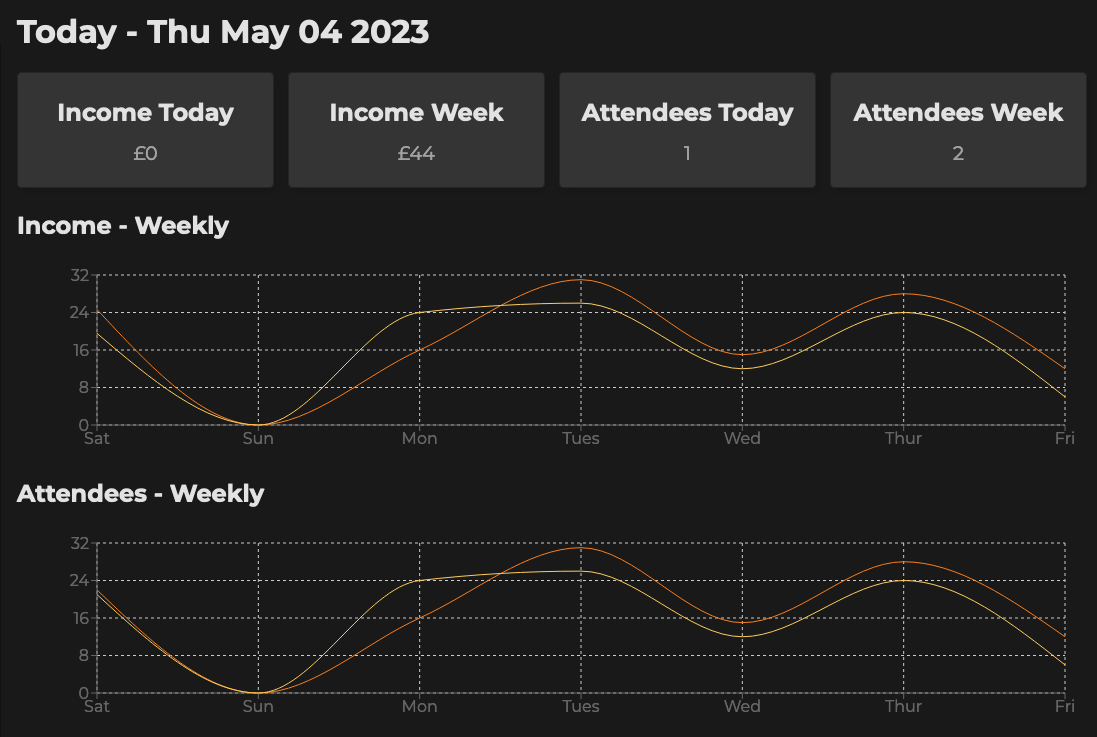
\includegraphics[width=.8\linewidth]{dashboard.png}}
    \caption{Dashboard implemented screen}
    \label{fig:dashboard-screen}
\end{figure}

For a more visual reprenstation of the data, two graphs were used to show the weekly income and attendances. Since these will closely correlate with each other, it will be clear to see the trends of both and compare them at a glance. To create these graphs the data must be retrieved from the database and formatted into a JSON object which can be used by the graphing library. The graphing library used was Chart.js which is a free open source library for creating graphs and charts. The library was chosen for its simplicity and ease of use. The data is displayed on the dashboard screen below the cards.


\subsection{Sprint 7 - Final Deployment}
For the final deployment, a domain name was aquired to provide a single point to access the web application. The domain name was purchased from name.com and the hosting was provided by Linode. The domain name was linked to the hosting by adding A records pointing to the Linode server host. The hosting was configured to run the web application using a virtual private server (VPS) running Ubuntu 20.04. The web application was deployed to the VPS using Git and the web server was configured to serve the application.

\begin{figure}[ht!]
    \centerline{\includegraphics[width=\linewidth]{server.png}}
    \caption{Server hosting the web application}
    \label{fig:server}
\end{figure}

The web server used was Nginx which is a free open source web server. The web server was configured to use a firewall to block all traffic except for the required ports. The web server was also configured to use a secure sockets layer (SSL) certificate to encrypt the traffic between the web server and the client.

The SSL certificate was provided by Let's Encrypt which is a free open source certificate authority. The SSL certificate was configured to automatically renew every 90 days. The web server was configured to redirect all HTTP traffic to HTTPS to ensure all traffic is encrypted.

\begin{figure}[ht!]
    \centerline{\includegraphics[width=.8\linewidth]{ssl.png}}
    \caption{Website secured with Let's Encrypt SSL certificate}
    \label{fig:ssl}
\end{figure}

\subsection{Sprint 8 - Bug Fixing and Report}
The final sprint was focused on bug fixing and writing the report. The bug fixes were focused on the issues that were found during the testing phase. These were quite few and far between thanks to regular unit tests on the developed components. The larger end-to-end tests results showed some inconsistencies when these components interacted together. This was valuable as the end-to-end operations are what the end user will be experiencing when interacting with the system. 

The report was written in LaTeX and was focused on the design and implementation of the web application from start to finish. Great care was taken to include all the details of the development process and the reasoning behind the decisions made. The report was also written in a way that it could be used as a guide for future developers to understand the system and how it was developed making futher development easier and more efficient.


%----------------------------------------------------------------------------------------
%	2. Software testing
%----------------------------------------------------------------------------------------

\section{Software testing}

Testing is vital to the development to ensure a high-quality user experience and prevent bugs and other inconsistencies from occurring within the system.

\subsection{Testing methods}
Testing can be approached from a black-box or white-box technique. Black-box testing is where only the inputs and outputs are of concern, with the internal structure unknown. In contrast, white-box testing reveals the inner workings of an operation, and further testing to interact with the internals is the focus.

Black-box testing is beneficial in the end-to-end validation of a function, operation or even user stories since it can provide a similar interaction that the end user will experience. Unfortunately, this testing is most commonly performed manually; each test is carried out by either the developer or a manual tester.

White-box testing focuses more on the functionality of smaller components within the system, such as algorithms and specific functions. Since the code is visible and followed, developers can use automated tests to guarantee that functions behave as expected.

In both methods, different parameters yield different functionality and responses from the application. These can exist as sunny-day scenarios where all inputs are what is expected, edge cases where the limits of inputs are tested but are still within bounds and finally, error scenarios where the input falls outside the expected parameters or is performed out of order.

\subsection{Code verification}
Before the system can even perform, the code must be functional and clean to ensure the system's sustainability for further development. Therefore, an editor with syntax highlighting is essential during development. Visual Studio Code provides built-in and downloadable syntax highlighting tools to check code on the fly for any typing or syntactical errors. Performing builds will also produce errors should the code be incorrect.

Linting tools such as ESLint can also be utilised to comb over the structure of the code by assisting with formatting and syntactical mistakes, which may still compile while resulting in unexpected behaviour. Fixes from linting tools may also restructure the code, making it easier to spot mistakes.

The prettier extension for visual studio code provided a restructuring functionality to make code easier to parse and spot potential mistakes through better tabbing. This tool was also used with ESLint to check the UI and API javascript code for syntactical and structuring mistakes.

\subsection{Database testing}
Manual white-box testing ensures that required data are required input fields. Custom SQL queries are written in the PgAdmin interface and then run against the specified tables, checking all sunny-day, edge and error cases.

\subsection{API testing}
White-box testing was performed on individual middleware and more complex operations, including manual testing of the token validation and database connection functionality.

The Black-box testing approach was used on end-to-end testing of each endpoint, utilising first OpenAPI documentation for sunny-day scenarios, then Postman with its ability to craft custom requests testing the fringes and error cases.

Further stress testing was performed on the endpoints to ensure they supported a greater throughput, potentially three staff members accessing the system at any given time. 

\subsection{UI testing}
Since the user interface remains a simple method of interaction, black-box end-to-end testing was conducted on the login system and, within the core application, each form input and button.


%----------------------------------------------------------------------------------------
%	3. Risk management
%----------------------------------------------------------------------------------------

\section{Risk management}
Risk management is the process of identifying potential risks to the software project and taking proactive measures to minimize their impact. This involves assessing the chance of each risk occurring, evaluating the potential impact on the project, and developing strategies to prevent or even mitigate the risk entirely.

\subsection{Mitigation plan}

A mitigation plan helps to proactively manage risks and reduce their impact on the project. It is an essential component of this project's development as it reduced many hiccups which occured throughout.

\begin{table}[ht!]
    \caption{Project mitigation plan}
    \renewcommand{\arraystretch}{1.5}
    \centerline{
        \begin{NiceTabular}{ m{2.5cm} m{2cm} m{4cm} m{4cm}  }
            \hline
            \textbf{Risk} & \textbf{Risk Type} & \textbf{Countermeasure} & \textbf{Action Plan}\\
            \hline \hline
            Unavailable resources & Cost & Ensure all resources are available early on & Request alternatives in the event of unavailability \\
            \hline
            Running out of time & Schedule & Schedule work within the time aloted with regular gaps to review and catch up  & Reduce superfluous features to meet the core requirements before the deadline \\
            \hline
            Non-implementable or impossible feature & Technical & Create prototypes in isolated projects with regular testing & Observe and create alternative implementations or instances of the feature \\
            \hline
            System failure & Technical & Create prototypes in isolated projects with regular testing & Observe and create alternative implementations or instances of the feature \\
            \hline
           \end{NiceTabular}
    }
    \label{fig:riskplan}
\end{table}

\subsection{Problems faced}

During the development of the MVP, issues were raised concerning access to the domain name since a subdomain for the application was requested. Since the managers purchased the website through a management company, there was no method of aquiring a subdomain to host the application. This was suitably managed through the mitigation plan through aquiring a new domain name for use to host the application. This was purchased through the business and setup to link with the VPS host of their choice.

Another problem which arose after the winter break was a personal issue which resulted in inconsistent work days and unavailability for meetings. This was mitigated through the mitigation plan by allowing the extra time for review to be used for development and by reducing the scope of the project to ensure the core requirements were met before the deadline. This was achieved through the use of a kanban board to track the progress of the project and ensure the core requirements were met before the deadline.


 % Project Management
%----------------------------------------------------------------------------------------
%	Professional isues
%----------------------------------------------------------------------------------------
\chapter{Professional issues} % Main chapter title
\label{Chapter6} % For referencing the chapter elsewhere, use \ref{Chapter6}

This section covers the professional issues concerned with the project, including the impact of legal requirements, the social implications of the software and the ethical code of conduct for the business when utilising the software.


%----------------------------------------------------------------------------------------
%	1. Data protection
%----------------------------------------------------------------------------------------

\section{Data protection}
The General Data Protection Regulation 2016 (GDPR) and Data Protection Act 2018 (DPA) laws require UK businesses to abide by specific criteria when working with customers' private, personally identifiable data. One of the core tenets is securing personal data against public access or attacks from malicious parties such as hackers. As a result, many methods were implemented and incorporated into the project's development to prevent the unnecessary transfer or collection of private data.


\subsection{Synthetic data}
During development and testing, synthetic data was used to remove the possibility of customer data being leaked through the project's version control system and deployments. With no access to the customer records, no prejudice or manipulation of data could occur. In combination with this, the customer's privacy is kept intact, which abides by the law. Using this data would require getting written permission from the business's customers.


\subsection{Data capture}
Another critical legal requirement component is minimising data captured for storage and only recording what is required for the business to operate. Excessive storage is detrimental to both the customer and the company. 

In the event of a breach, the impact would be worse than necessary since more private information could be exposed. More insidious would be using this data to target individuals, which is invasive and could endanger the customer.

This is also not beneficial as a business proposition. The higher requirement for customers when working with the business combined with higher running costs for collection and storage would result in customer dissatisfaction and increased business expenses.


\subsection{Data retention}
According to the Companies Act 2006 \parencite{participation_companies_nodate}, a business must hold financial records for at least six years. These accounts are currently compiled from the till receipt carbon copies. This compilation is time-consuming and requires recalculating every month and year.

The developed system is more than capable of storing this information almost indefinitely. Moreover, the data can be recalculated nearly instantaneously and for any time range asked. Since the data must be sent in tax returns, there will always be two copies of the financial records in case an audit is required.


%----------------------------------------------------------------------------------------
%	2. Software security
%----------------------------------------------------------------------------------------

\section{Software security}
The software must be secure to abide by the legal requirements of keeping the data safe. Therefore, multiple methods and measures were taken to ensure the data was not accessible without authentication and verification of identity.

The login system provides the first layer of protection through access control. The interface is not accessible for making requests to the API, preventing the majority of the general public from clicking through and requesting data. 

The API provides the second layer. Endpoints that access data require a valid JSON Web Token issued by the server to complete the request successfully. In combination, the queries are predefined to prevent querying for unauthorised data.

Finally, the database is completely isolated from the public internet, making it the third and final layer. The connection would require hacking the server where the data is stored and cracking the login details.


\subsection{Secure data transfer}
Since the data is transmitted from potentially unsafe connections, data must be transferred securely to prevent an attacker from capturing the information in transit.

The server is configured with SSL encryption through a server application called CertBot. This software generates a certificate through Let's Encrypt, a public, free-to-use certificate service to secure websites. The certificate is generated for the domain name and allows the data sent to be encrypted and sent to the server. There, the data can be unencrypted for actions to be performed.

To bypass this security, the attacker would need access to the server to intercept the requests. So at this point, the issue would no longer be in the transmission security but in the server's security.


\subsection{SQL injection attack}
An SQL injection attack is a carefully crafted request that bypasses the original query and returns different data from other locations in the database. This is a tactic many hackers and penetration testers use to attempt to access a networked system.

The Upgrade CRM system actively prevents these injection attacks by validating incoming requests through the API. The values are passed through checks to ensure the data is valid and special characters often used in this attack are escaped.


\subsection{Server hacking}
The server is another point of attack which a malicious actor may want to try compromising. An attempt could be password guessing. The number of attempts is inconsequential since password access is disabled from use. Only keys are used to access the system and only as a non-privileged user. To perform admin tasks, the user must know the admin password, which would require slow attempts, and access logs would show a new logged-in user from their connection location.


\subsection{Vulnerabilities}
Over time new vulnerabilities are discovered in existing systems, such as operating systems and software packages.

To combat this in deployment, the server uses automatic updates configured to download and update when new security updates are available. In addition, the server restarts are automated to run at 3 am to prevent potential downtime during work hours.

As for the packages used in the React interface and NodeJS API, GitHub supports the monitoring of projects through a bot. This bot provides more than just monitoring but also updates through a new git branch which can be merged into the main branch. By using a different branch, a developer can perform a code review before implementing the patch or fix. 


%----------------------------------------------------------------------------------------
%	3. Ethical concerns
%----------------------------------------------------------------------------------------
\section{Ethical concerns}
A business has a responsibility and legal obligation to keep the customer in mind when operating.

Spam emails have been a concern since its wide adoption in the early 2000s. As a result, in recent years there have been requirements to allow recipients of marketing emails the option to unsubscribe from mailing lists. 

The application tracks member emails for contact about pricing updates and special events. Members can request to avoid being contacted via email through their member details.
 % Professional Issues
%----------------------------------------------------------------------------------------
%	Conclusion
%----------------------------------------------------------------------------------------
\chapter{Conclusion} % Main chapter title
\label{Chapter7} % For referencing the chapter elsewhere, use \ref{Chapter7}

%----------------------------------------------------------------------------------------
%	1. Project summary
%----------------------------------------------------------------------------------------

\section{Project summary}

The problem this project was created to resolve was to support a local gym which offers boxing, kickboxing and yoga services which is outgrowing their current system of tracking customers, their payments and attendance for lessons. The proposed solution was to create an online software which allows entry of member data, tracking of purchases and attendances for lessons while providing useful metrics for member signups, attendance and payments over several time scales.

Overall, this project has been a great success with results that have been overwhelming. The solution has been a comprehensive software capable of scaling as they grow while remaining simple for receptionists, coaches and managers to interact with.

The system also provides valuable, useful statistics for the business managers to make more informed business decisions. The accurate financial data has given the managers enough information to know if moving into another larger location is viable to accommodate the influx of members.

The improved and unified system has saved a great deal of time for the receptionist. She is now able to relax more with reduced pressure to remember customer information and is also able to perform other gym related tasks to assist the coaches.

A large component of this project which has resulted in this success has been through project planning and in depth discovery sessions which revealed the system requirements early on making focus during development far easier.

Research and planning also had a large impact on the efficiency of development. Having searched alternative products available on the market and effective design patterns for system architecture provided useful design and feature designs while reducing potentially wasted time reiterating over a more complex feature.


%----------------------------------------------------------------------------------------
%	2. Personal reflection
%----------------------------------------------------------------------------------------

\section{Personal reflection}

Although the project has been a success, there have been a few points where the process and resulting implementation could have been managed and worked on better.

Regular commits to the GitHub repository to better show progress over time and allow more flexibility in reversing any bugs or mistakes made. In combination with this, better use of branches for new features would have also contributed to a more efficient development process.

Having a developer's perspective of the software, some features which the managers and coaches may require were missed in the planning stages resulting in a less flexible system. One major oversight was in updating the prices for lessons. This was partially remedied through a new route being added to manually change the prices however would still require a developer to perform the change.

Meetings and time tracking at the beginning of the project was clear and simple. As development started and more complex features were being added, maintaining regularity and balancing workloads for other modules resulted in a less consistent development cycle which had a more significant impact when time had to be taken away for personal reasons. This created undue pressure where the mitigation plan was stressed beyond the planned mitigation.

If I was to work on this project or another project of this scale, I would make a few changes to my process and methodology for development.

The first would be the use of a protected main branch for the GitHub repository. This would have remedied the issues concerning regular and atomic commits where all changes would be tracked in their own smaller branches. The review time would be greatly reduced making for a more efficient and speedy development with as good or higher quality results.

Testing during and after development took a lot longer than anticipated. Planning around this through more time alotted to this task would be beneficial combined with time spent creating more automated testing. This would pay dividends as time goes on for a project where small components can be guaranteed to work.

Finally, a greater focus on the core functional features would have saved much time and work. With the functionality complete, user experience could be focused on with greater attention resulting in a far superior and user focused approach.

The University of Brighton has provided a great number of valuable modules which have contributed to the development of such a useful application. 

Web development during the full three years of study has given a solid foundation to build upon with valuable insights into the industry, best practices and functional tutorials.

Design patterns and system architecture was a module missing from my past knowledge and experience working in the industry. This module provided a focus on how to structure a product rather than build it. This key shift in focus has provided an effective angle to work from making larger projects more manageable.

The second year group project was eye opening to the requirements and needs of a project from a management perspective. Managing time and resources including other members of a team is vital for the creation of a complex system. This emphasises the planning and research phase of development showing how valuable a blueprint is to work from.

Private and individual study has been a huge benefit for me as no lecture, lab or module can provide all the necessary information for working on a project or in the industry. Experience working in the industry through a scholarship has garnered vast experience when in a professional setting. Considerations for customers and other developers is something that is not highly regarded in an academic setting.

Building personal project for both myself and private customers allows the implementation of the skills learned and provide a useful metric to see what knowledge you are lacking and an outlet to search for the solution.

%----------------------------------------------------------------------------------------
%	3. Future work
%----------------------------------------------------------------------------------------

\section{Future work}

The future of this project is bright with many features and improvements planned for the future. The current system is a great foundation to build upon with many features already planned and in development. The following is a list of features which are planned for the future.

\begin{itemize}
    \item Item purchases
    \item Basket system
    \item Hardware access for replacing till
\end{itemize}

The item purchases feature will allow the gym to track the sales of items such as gloves, wraps and other equipment. This will be a simple feature which will allow the receptionist to add items to a basket and checkout the customer with the selected items.

By allowing access to hardware such as till receipt printers, bar code scanners and cash draw will allow the gym to replace their current till system with the new software. This will allow the gym to have a single system for all their needs further unifying the systems and providing greater metrics.

Other concerns may become a concern such as multi-site and multi-gym support. This would require a more complex system to be developed to allow for the management of multiple sites and gyms. This would be a large undertaking and would require a great deal of planning and research to ensure the system is flexible enough to support the needs of the gym. These are all considerations which can be made in the future as the gym grows and expands in the years to come.
 % Conclusion

%----------------------------------------------------------------------------------------
%	BIBLIOGRAPHY
%----------------------------------------------------------------------------------------

\printbibliography[heading=bibintoc]

%----------------------------------------------------------------------------------------
%	THESIS CONTENT - APPENDICES
%----------------------------------------------------------------------------------------

\appendix % Cue to tell LaTeX that the following "chapters" are Appendices

% Include the appendices of the thesis as separate files from the Appendices folder
% Uncomment the lines as you write the Appendices

% Appendix A

\chapter{Project Links} % Main appendix title

\label{AppendixA} % For referencing this appendix elsewhere, use \ref{AppendixA}

\section{Github}\label{AppendixA:Github}

\href{https://github.com/jazerbarclay/ci601-upgrade}{https://github.com/jazerbarclay/ci601-upgrade}


\section{Deployemnt}\label{AppendixA:Deploy}

\href{https://app.upgrade-crm.com/}{https://app.upgrade-crm.com/}


\section{Trello}\label{AppendixA:Trello}

\href{https://trello.com/b/xphHSfcJ/ci601-final-year-project}{https://trello.com/b/xphHSfcJ/ci601-final-year-project}


\section{Trello}\label{AppendixA:Gantt}

\centerline{\includegraphics[width=\linewidth]{gantt1.png}}

\centerline{\includegraphics[width=\linewidth]{gantt2.png}}
% Appendix B

\chapter{Supervisor Meeting Notes} % Main appendix title

\label{AppendixB} % For referencing this appendix elsewhere, use \ref{AppendixB}

Appendix A includes a summary of events from each meeting including an action to be focused upon for the following meeting.

\section{5th October 2022}
\begin{itemize}
    \item Call agreed Khuong to be supervisor for this project
    \item Project ideas were presented
    \item Project was selected and agreed with supervisor
    \item LaTeX was recommended to be used when starting interim report
    \item Action: Start on the project code and check in progress in next meeting
\end{itemize}

\section{12th October 2022}
\begin{itemize}
    \item Call with Khuong to check in with current progress
    \item Advice requested for Ethics form regarding live and synthetic data
    \item Advised to aquire written consent from business for use of assets such as logos and other copyrighted material
    \item Action: Prepart documents for project proposal submission
\end{itemize}

\section{24th October 2022}
\begin{itemize}
    \item Call to check in with current progress on development
    \item Discussed system architecture and development process
    \item Questions raised regarding technical complexity
    \item Overview provided for interim report
    \item Action: Look at including more technical compledity in the project
\end{itemize}

\section{7th November 2022}
\begin{itemize}
    \item Discussed marking criteria for interim report
    \item Covered more detail and recommended layout
    \item Action: Focus on interim report
\end{itemize}

\section{21st November 2022}
\begin{itemize}
    \item Call with Khuong about viva presentation
    \item Looked at requirements for viva
    \item Discussed presentation layouts and other recommendations
    \item Action: Prepare for viva with presentation and report
\end{itemize}

\section{7th December 2022}
\begin{itemize}
    \item Check in for update on viva presentation
    \item Examined feedback form for any missing details
    \item Action: Complete presentation slides ready for meeting with second reader
\end{itemize}


\section{14th December 2022}
\begin{itemize}
    \item Viva presentation with Khuong and second reader Saeed
    \item Feedback provided after meeting
    \item Updated Khuong with development progress
    \item Action: Aim to complete work by end of January to early February
\end{itemize}

\section{19th December 2022}
\begin{itemize}
    \item Check in for update on viva presentation
    \item Examined feedback form for any missing details
    \item Action: Complete presentation slides ready for meeting with second reader
\end{itemize}


\section{17th January 2023}
\begin{itemize}
    \item Update on progress
    \item Push for completing work before end of Feb
    \item Noted to focus on report asap
\end{itemize}

\section{27th March 2023}
\begin{itemize}
    \item Update on progress
    \item Focused on bug fixes and report
    \item Covered marking criteria
    \item Provided with thesis template
    \item Recommended use of LaTeX for report
\end{itemize}

\section{4th April 2023}
\begin{itemize}
    \item Covered dissertation outline
    \item Discussed additional content and research
\end{itemize}

\section{11th April 2023}
\begin{itemize}
    \item Went into greater depth of the structure
    \item Discussed word count, appendix and references
\end{itemize}

\section{18th April 2023}
\begin{itemize}
    \item Presented first 4 chapters of the report
    \item Discussed additional content and research
    \item Action: Refactor first 4 chapters using feedback
\end{itemize}

\section{25th April 2023}
\begin{itemize}
    \item Presented additional chapters for review
    \item Feedback received including use of more references
    \item Action: Refactor report to include more references and additional figures
\end{itemize}

\section{2nd May 2023}
\begin{itemize}
    \item Final meeting
    \item Discussed final changes and feedback
    \item Action: Complete final changes and submit report
\end{itemize}


% Appendix C

\chapter{Business Documents and Assets} % Main appendix title

\label{AppendixC} % For referencing this appendix elsewhere, use \ref{AppendixC}

Appendix C includes all documentation, assets and other resources received from Up-grade Martial Arts used in the support of the creation of this software artefact.


\section{Logo}\label{AppendixC:Logo}

\centerline{\includegraphics[width=0.45\linewidth]{uma-logo.png}}


\section{Colour scheme}\label{AppendixC:ColourScheme}

\centerline{\includegraphics[width=.6\linewidth]{colours.png}}


\section{Signup form}\label{AppendixC:SignupForm}

\centerline{\includegraphics[width=\linewidth]{signupform.png}}


\section{Price list}\label{AppendixC:PriceList}

\centerline{\includegraphics[width=\linewidth]{upgrade-price-list.png}}


\section{Attendance Spreadsheet Sample}\label{AppendixC:AttendanceSpreadsheet}

\centerline{\includegraphics[width=\linewidth]{attendance-ex.png}}


\section{Website}\label{AppendixC:Website}

\href{https://www.upgrademartialarts.co.uk/}{https://www.upgrademartialarts.co.uk/}

\centerline{\includegraphics[width=\linewidth]{website.png}}

%----------------------------------------------------------------------------------------

\end{document}  
